\documentclass[12pt,oneside]{book}
\pagestyle{headings}

% Note that the line below could be modified to suit a
% particular system since the "geometry" package behaves
% differently in Unix, Windows and Mac, especially for the
% top margins.
% Adjust the parameter "top" (measuring the height of the
% space allocated to a header) and "headsep" (measuring
% the distance from the bottom of the header to the
% first line of text.
\usepackage[top=1.3in,left=1.5in,bottom=1in,right=1in,headsep=0.5in]{geometry}

\usepackage{setspace}
\onehalfspacing
%\doublespacing

% Headers and footers for thesis
\usepackage{fancyhdr}

\markboth{}{}
\newcommand\startchapter[1]{\chapter{#1}\thispagestyle{myheadings}}
\newcommand\startappendix[1]{\chapter{#1}\thispagestyle{myheadings}}
\newcommand\startfirstchapter[1]{\chapter{#1}}

% Manual addition of section to Table of Contents
\newcommand\TOCadd[1]{\newpage\phantomsection\addcontentsline{toc}{chapter}{#1}}

% Float Customization
\renewcommand{\floatpagefraction}{0.01}

% Customization of Tables of Contents and List of Figures/Tables
\usepackage{subfigure}
\usepackage[subfigure]{tocloft}

\renewcommand\cfttabpresnum{Table\ }
\renewcommand\cfttabnumwidth{0.75in}
\renewcommand\cftfigpresnum{Figure\ }
\renewcommand\cftfignumwidth{0.80in}
\newcommand{\HRule}{\rule{\linewidth}{0.5mm}}

% Block quotes
\usepackage{etoolbox}
\AtBeginEnvironment{quote}{\par\singlespacing\small}

% Long Table and decimal aligned columns
\usepackage{dcolumn}
\usepackage{longtable}

% Mathematics support
\usepackage{amsmath}
\usepackage{amsthm}
\usepackage{amssymb}


% Text Control
\usepackage{xspace}
\usepackage{textcase}

% Graphics
\usepackage{wasysym}
\usepackage{graphics}
\usepackage{graphicx}   % A package to allow insertion of
                        % external image files

% Additional required
\usepackage{url}
\usepackage{threeparttable}
\usepackage{multirow}
\usepackage{booktabs}
\usepackage{hyperref}           % clickable references and URLs

% Setup for code listings

% Required for Texpad, remove outputdir for overleaf
\usepackage[outputdir=.texpadtmp]{minted}

\usepackage{xcolor}

\definecolor{bg_minted}{rgb}{0.95,0.95,0.95}
\definecolor{bg_inline}{rgb}{1.0,1.0,1.0}
\setminted[python]{xleftmargin=2pt, linenos, tabsize=4}
\setmintedinline[python]{bgcolor={}}

% Framing around code blocks
\usepackage{mdframed}
\mdfdefinestyle{MyFrame}{%
    linecolor=black,
    outerlinewidth=2pt,
    innertopmargin=6pt,
    innerbottommargin=6pt,
    innerleftmargin=0pt,
    innerrightmargin=0pt,
    backgroundcolor=bg_minted,
    leftline=false,
    rightline=false
}
\surroundwithmdframed[style=MyFrame]{minted}

\begin{document}

% Front Matter
\input frontmatter/fm

\newpage

	\startfirstchapter{Introduction}

"I automate whatever can be automated to be freer to focus on those aspects of music that can't be automated. The challenge is to figure out which is which." \cite{hinkle2006women}

\begin{enumerate}
    \item Introduction to the problem of programming synthesizers
    \item overview of some of the various techniques that have been taken. Break the problem down into a couple of different components: the backend problem and the frontend. A lot of resources have been placed in the backend and deep learning / neural networks have played a large role in this.
    \item We look at a couple different approaches to the backend problem: inverse synthesis, neural synthesis (what does wavenet do?)
    \item Introduce DDSP and present torchsynth, a synthesizer built to support future machine learning work in this area.
    \item Inverse synthesizer experiment using torchsynth -> Even if it is just a genetic algorithm or something like that. Is there a way to explore the GAN approach for this too?
    \item Single knob attachment to torchsynth? UMAP style?
    \item Sound exploration interface for torchsynth (or any other synthesizer really)
    \item Conclusion (what have we learned from this? What are the next steps)
    
\end{enumerate}

\label{chapter:introduction}

% My main statement about the introduction is:
% \textit{"keep it short and write it last".} The main features should be as follows:
% \begin{enumerate}
% \item {3-4 pages at most;}
% \item {Start with a VERY short statement of the problem (2-3 sentences) - the problem should be stated, not described, as there will be a whole chapter for that;}
% \item {State why the problem is important, its impact, how well it has been studied recently, its application (3 sentences) - this should be again a brief motivation, leaving a full impact description to later in the document;}
% \item {Give a sketch of the new approach - there will be a whole chapter with all the details, now just impress the reader about what is the new approach, just as you would do if your boss asked you at work during an elevator ride;}
% \item {Sketch the main new ideas of the new approach - again briefly, just get the reader interested;}
% \item {Give a short statement regarding the results, nothing too elaborate, but certainly you should blow your horn and make sure that the reader is intrigued;}
% \item {Interspersed in all the writing above do not forget the marketing angle, trying to suggest forcefully why the reader should keep reading;}
% \item {Give an outline of what is to come in the organization of the thesis overall - you will find one below for this document.}

% \end{enumerate}

% Finally the strong suggestion is write the introduction chapter last. It will be faster, you will know what to say as the rest is already there, and the abstract, introduction and conclusion will be a mirror and complement of each other. You may well ask where to start writing your thesis. My view is included in the organization below.


Automated methods for music production -- why do we need it? The main thread here is looking at methods for exploring sound spaces. How can we improve this approach? Potentially need a bit on timbre -- the timbre space article could be really good.

General introduction. Distinction between creative mir, intelligent music production, automatic synthesizer programming.

Democratization of sound \cite{tavana2015democracy}

Moffat and Sandler examine approaches to intelligent music production \cite{moffat2019approaches}.

\cite{krekovic2019insights} user study examined synthesizer user habits and pointing to need for further work in automatic synthesizer programming

\section{Automating Synthesizers}
The use of sound synthesizers in the fields of music composition, production, and performance is widespread, but the task of programming a synthesizer is complex and requires a thorough understanding of technical details. It is not uncommon for a software synthesizer to have 30+ parameters displayed on a user interface (UI) and labelled using technical names \cite{rasmussen2018evaluating}. Manually programming sounds using such a large set of parameters is a daunting task. Synthesizer programming is further complicated by the fact that modifications to parameters are often not intuitively reflected in the end sonic result. This disconnect can be disruptive to the creative process. Automatic synthesizer programming (ASP) is the field of research focused on addressing these challenges in programming synthesizers.

 Early ASP research emerged in the late 1970s with work that focused on the use of analytic methods to estimate the parameters for frequency modulation (FM) synthesis \cite{justice1979analytic}. That work was an example of synthesizer sound matching in which a system estimates synthesizer parameters to replicate a target sound. Since then a large volume of work on synthesizer sound matching has been published and has explored a variety of synthesis techniques and algorithmic methods. One popular approach is the use of evolutionary algorithms \cite{horner1993machine, mitchell2007evolutionary, yee2007evolving, yee2008synthbot, heise2009automatic, roth2011comparison, tatar2016automatic, smith2017play}. More recently, deep learning techniques have been explored \cite{yee2018automatic, barkan2019inversynth, esling2020flow}. Other methods that have been studied include semantic descriptions \cite{ethington1994seawave, johnson2006timbre, krekovic2016algorithm}, interactive methods \cite{johnson1999exploring, dahlstedt2001creating, yee2016use}, and sound matching with vocal imitations \cite{mcartwright2014, zhang2018visualization}.
 
 A recent user study conducted by Krekovi{\'c} et al. confirmed the desire among synthesizer users for improved means of working with their synthesizers \cite{krekovic2019insights}. 
 %Users identified approaches they felt would be particularly beneficial, which included automatic sound matching and improvements to user interface design. 
 While recent research has produced promising results, automatically programming a modern software synthesizer still presents challenges. Current evolutionary techniques face issues including time complexity \cite{tatar2016automatic}, while recent deep learning approaches have challenges in consistently producing accurate reproductions \cite{yee2018automatic}. The desires expressed by the users in Krekovi{\'c} et al.'s study, coupled with the need for further research and improvement noted in the existing body of work, point to the need for further development in ASP.
 
 The work presented here attempts to continue this development, and promote collaboration and reproducibility in ASP research through the introduction of \mintinline{python}{spiegelib}, an open-source library written in the Python programming language. Vandewalle et al. argue that reproducibility in computational science research increases the impact of a work and they provide a framework for evaluating the quality of reproducibility \cite{vandewalle2009reproducible}. The aim of \mintinline{python}{spiegelib} is to provide a platform for researchers of automatic synthesizer programming to develop, test, and share implementations in a way that promotes reproducibility at the highest level. \mintinline{python}{spiegelib} stands for Synthesizer Programming with Intelligent Exploration, Generation, and Evaluation Library. The name \mintinline{python}{spiegelib} was chosen to pay homage to Laurie Spiegel, an early pioneer in electronic music composition. Laurie Spiegel is known for utilizing synthesizers and software to automate certain aspects of the music composition process. Her philosophy for using technology in music serves as a motivation for the \mintinline{python}{spiegelib} software library: "I automate whatever can be automated to be freer to focus on those aspects of music that can't be automated. The challenge is to figure out which is which." \cite{hinkle2006women}


Introduce automatic synthesizer programming. Tie it to intelligent music production \cite{moffat2019approaches} \cite{de2017ten} and creative MIR \cite{humphrey2013brief}.

\subsection{History}
DX7 plays an important role here - made synthesizers more widely available but programming them was notoriously difficult. 9 out of 10 DX7s that went in for service had factory presets intact (Reference needed). Almost immediately researchers became interested in learning how to estimate synthesizer presets for FM algorithms which spread into non-linear synthesis methods, then wavetable synthesis, then physical modelling, granular, additive. (References needed for synthesis types). 

Justice 1979 \cite{justice1979analytic}  - Automatic FM matching. Early example of looking try to find a coarse match of FM generated tone to the parameters (ie examples were FM generated). Beauchamp 1982 \cite{beauchamp1982synthesis} - Frequency domain matching of FM tones. Included in a larger study involving spectral centroid matching in nonlinear synthesis. Early automatic spectral match. Also looked at non-linear and filter model. Found that non-linear/filter model worked better. Payne 1987 \cite{payne1987microcomputer} Looked at automatic FM tone matching to the acoustic sounds - using DX7 and hilbert transform as well. Delprat et al. 1990 \cite{delprat1990parameter} using wavelets for non-linear synthesis parameter estimation. Horner at al. early example of automatic synthesizer preset generation in 1993 \cite{horner1993machine}. Attempted to match FM parameters with a harmonic signal using a genetic algorithm. Horner et al. then applied denetic algorithm applied to wavetable synthesis \cite{horner1993methods}. Vouri and V{\"a}lim{\"a}ki on parameter estimation for physical modelling of flute tones \cite{vuori1993parameter}. Fujinaga and Vantomme 1994 Genetic Algorithms applied to granular synthesis \cite{fujinaga1994genetic}. SeaWave by Ethington and Punch, a synthesizer that can be controlled using vocabulary. Has a pre-defined set of descriptors \cite{ethington1994seawave}. Miranda 1995 paper proposing a system utilizing AI to automatically program a generic synth using vocabulary \cite{miranda1995artificial}. Horner 2003 paper reviews FM and wavetable synthesis as well as approaches to automatic parameter matching \cite{horner2003auto}.


\section{User Interface Design}
\subsection{Synthesizer Programming}
Seago identified disconnect between the language of users and the language used in synthesizer interfaces \cite{seago2004critical}. Recent work focussed on synthesizer UIs \cite{rasmussen2018evaluating}. Krekovic in a 2019 study of 112 synthesizer users, reported most participants reported feeling like the process of modifying or creating new synthesizer patches was a challenging process and not intuitive \cite{krekovic2019insights}. A majority of users' felt like more intuitive interfaces was the area that would be most beneficial in helping them during the process of programming a synth. Users also felt that sound matching would be helpful. Krekovic identifies that relatively little research has been completed in the area of synthesizer user interfaces. This is reflective of recent research focussed on human computer interface and ui design for music applications \cite{pardo2019learning}\cite{knees2019intelligent}.
	\chapter{Background}
\label{chapter:background}
- Research in this field is inherently interdisciplinary background covers many different areas including HCI, DSP, Machine learning
- What is the main goal? Reiterate here perhaps: "We want to develop a method for improving the user interface for synthesizer users" -- 
- In the field of HCI the study of creativity support tools is related to this:

\graphicspath{{./}{./figures/}{./figures/background/}}

\section{Audio Synthesizers}
In the context of audio, a synthesizer refers to a device that generates sound or music. Martin Russ provides a thorough overview of audio synthesis in his textbook, Sound Synthesis and Sampling \cite{russ2012sound}. Russ introduces the synthesizer as any device that gerates sound,  even the human voice can be thought of as a synthesizer, however, sound synthesizers have become more broadly accepted as an electronic device that produces synthetic sounds. A synthesizer may do this through the playback and recombination of pre-existing audio material or through the generation of raw audio waveforms. There are numerous types of synthesis techniques that are capable of producing a huge variety of different sounds. Broadly speaking, these sounds can be categorized into two different classes: `imitative` or `synthetic`. Imitative sounds attempt to emulate a sound that exists in the natural world such as a physical musical instrument or a sound effect such as an explosion. Electric pianos are examples of imitative synthesizers. Synthetic sounds are those that have no relation to a sound in the physical world. The distinction between imitative and synthetic sounds is blurry and most sounds fall somewhere in the middle. For example, synth-brass sounds, which were a staple of synths such as Roland's popular Jupiter-8, are sounds that are based on an imitation of a brass sound but extend into the synthetic realm. 

% This is maybe a bit more like introduction material?
Synthesizers have become ubiquitous in audio production and entire genres of music have been developed around their use. Bebe and Louis Barron produced the first electronic film score for the movie "Forbidden Planet" in 1955 using synthetic sounds. Since then the use of synthesizers for movies and video games has also become common-place.


\subsection{Evolution of Synthesizers}
A brief history of synthesizers is provided here for historical context to the development and use of synthesizers. The full history of the topic is beyond the scope of this thesis and the interested reader is referred to some great textbooks that cover audio synthesizers and their history \cite{roads1980interview, mcguire2015musical, jenkins2019analog, russ2012sound}, which were used in the writing of this chapter.
\subsubsection{Analog}
Until the late 1950s all synthesizers were analog. All analog synthesizers are defined by their use of continuous-time signals, as opposed to digital systems which operate in discrete chunks of information, or discrete-time signals. Early analog synthesizers can be broken down into two broad categories: (1) sounds that are generated directly by electric circuits by oscillating vaccuum tubes, or (2) rotating or vibrating physical systems that are controlled by electronic sources \cite{roads1996computer}. The first, as well as the largest sound synthesizer ever built was developed in the early 1900s by Thaddeus Cahill. On September 26, 1906, an audience of 900 individuals came to view the massive electronic instrument called the Telharmonium that was capable of producing pure sinusoidal waves in at frequencies in integer ratios. Other early synthesizers include the Theremin, built by Leon Theremin in 1920, which produced a pure tone with a varying pitch and amplitude that was controlled by a performer moving their arms in relation to two antennas. The sound produced by the theremin has an eery feel to it, well-suited for sci-fi film scores. Versions of the theremin have been used in popular music by musicians including The Beach Boys, Led Zeppelin, and The Rolling Stones (citations? check out wikpedia).  The Ondes Martenot, developed in 1928 by Maurice Martenot and Ondes, had a similar sound to the theremin and also was one of the first synthesizers to include a piano-like keyboard interface.

In the 1960s two companies emerged on opposite sides of America and released synthesizers that have shaped the landscape of audio synthesis. Around 1964 Don Buchla, who lived in the San Francisco area, released the the Buchla 100 Series Modular Electronic Music System and Robert Moog, who lived in the New York area, released the R.A. Moog Modular System \cite{mcguire2015musical}. Both synthesizers were modular systems that had individual processing units called \textit{modules} that could be interconnected using patch cables, connecting together synthesizer modules is known as creating a "synth patch", or simply a "patch". Both systems also include Voltage-Controlled Oscillators (VCOs) which create electronic waveforms at stable musical pitches, and the pitch can be controlled via an input signal. The Moog Modular System also featured a Voltage Controlled Filter (VCF) that was an early version of Moog's famous ladder filter design that would resonate at a controllable center frequency, creating some of the most iconic synthesizer sounds that are still used today.

There were some important philosophical differences between Moog and Buchla Synthesizers that have lead to two different schools of thought: East Coast and West Coast synthesis. The development of the Buchla synthesizer by Don Buchla was guided by Morton Subotnick and other experimental composers working out the San Francisco Tape Music Center. Subotnick explicitly requested that the synthesizer was not controlled by a traditional keyboard interface as he was worried that it would trap him into created tonal music. Instead, Buchla synthesizers are controlled using a set of touch plates and sequencers. At the same time on East coast Robert Moog was developing the Moog Modular and building a traditional keyboard interface to control the pitch of his VCOs. This feature, which allowed the Moog Modular Systems to be integrated more easily with Western music, was one of the reasons that Moog synthesizers became much more popular and commercially successful compared to Buchla. 

Another reason that Moog synthesizers were launched into the public eye is because of their use in recorded music. In 1968 Wendy Carlos used a Moog Modular synthesizer to orchestrate, perform, and record a selection of Johann Sebastian Bach pieces. The collection of music, called \textit{Switched On Bach}, went on to become the best selling classical recording of all time. Other musicians had created recreations of classical music pieces on synthesizers, but none had reached the same level as \textit{Switch On Bach}. Jenkins \cite{jenkins2019analog} credits the nature of the counterpoint in Bach's pieces as being particularly well suited to synthesizers, as well as Carlos' ability to design sounds that brought that performance alive, to the success of the release. Building on this success Carlos went on to score synthesized soundtracks for movies including Stanley Kubrick's \textit{A Clockwork Orange}. Another exceptional example of classical music recreated using Moog synthesizers worth mentioning is Japanese composer Isao Tomita's \textit{Snowflakes Are Dancing}, which was released in 1974. The use of synthesizers in music and film extends into almost all genres of music and was the cornerstone in the development of new genres including techno and other electronic music genres. [Also note something about the historical context and other synthesizer manufacturers] -> Mark Jenkins provides an excellent overview of the use of synthesizers in various genres of music over the years in his book \textit{Analog Synthesizers: Understanding, Performing, Buying} \cite{jenkins2019analog}.

\subsubsection{Digital}
The first experiments with digit synthesis were conducted by Max Mathews on an IBM 704 computer in 1957 \cite{roads1980interview}. These experiments consisted of programming and synthesizing melodies using triangle waves, Mathew's program was able to accept the note pitch, amplitude, and duration. The Music III program was developed by Mathew's in 1960 and introduced an important concept called the \textit{unit generator}, which defined basic components of a synthesizer in programmatic units that a user was able to link together to create a full synthesizer architecture. Mathew's describes these concepts as being developed in parallel, but separately, to similar synthesis concepts (e.g. modular synthesizers) being developed in the analog world. He described this as "an advantage because a musician who knew who to patch together Moog synthesizer units would have a pretty good idea how to put together unit generators in the computer."

In 1973 John Chowning, a researcher at Stanford, released a landmark audio synthesis paper entitled on Frequency Modulation (FM) synthesis \cite{chowning1973synthesis}. The patent for FM synthesis was licensed to Yamaha who developed the Yamaha DX7 synthesizer using the technology, which was released in 1983 and became one of the best selling synthesizers of all time. One of the major benefits of FM synthesis is that it is able to produce complex audio waveforms at low computational cost. Additionally, the Yamaha DX7 was a fully polyphonic synthesizer, meaning that it was capable of producing multiple tones simultaneously (i.e. was able to play chords), whereas most analog synthesizers that were within the same time period were monophonic (only capable of playing one note at a time). The Yamaha DX7 was also incredibly difficult to program, although it came preloaded with a large selection of quality parameter settings, or presets, that allowed users to play the synth without have to learn how to program it.

As digital technology improved and computers became more powerful, new synthesis techniques such a sampling synthesis \cite{mcguire2015musical} and physical modelling \cite{jaffe1983extensions} emerged. Digital emulations of analog synthesizers, or virtual analog (VA) synthesis, also started to become popular in the 1990s. VA synthesizers attempt to express traditional analog synthesis methods in code as digital signal processing (DSP) algorithms. The development of more powerful computers also enabled recording workflows to be transferred into software and professional recording studios started to transition to digital with the release of Digidesign ProTools in the early 1990s. As software synthesis became more prevalent, many types of different software synthesizers emerged including VA software synthesis and a trend emerged of directly emulating analog equipment digitally, including the user interface. Skeumorphism describes computer user interfaces that attempt directly mimic their real-world counterpoint, and has become extremely common in audio software, including synthesizers; user interface researchers have begun to question whether or not these skeumorphic interfaces enhance usability of not \cite{lindh2018beyond}.

\subsubsection{Audio Plugins}
In 1996 Steinberg\footnote{\url{https://www.steinberg.net}} released the Virtual Studio Technology (VST) interface, which allowed third-party software including audio effects to be integrated into host applications including DAWs. Because VSTs integrate with host applications, they are also called audio plug-ins. The second version of VST was released in 1999 which added support for the Musical Instrument Digital Interface (MIDI) \cite{rothstein1992midi}, a communication protocol enabling musical hardware and software to exchange information and control signals. The addition of MIDI to the VST interface opened the doors for VSTi, VST instruments, including software synthesizers. Other audio plug-in architectures have been developed in addition to VSTs, and popular ones include Apple's Audio Units (AU) and Avid's Avid Audio eXtension (AAX). Audio plug-ins have allowed software developers a method to create unique audio effects and synthesizers, and an industry dedicated to their development has blossomed over the last few decades. At the time of writing there are over 500 different synthesizer plug-ins available for purchase or for free on the KVR\footnote{\url{https://www.kvraudio.com/plugins/softsynth-virtual-instruments}} database of audio products.

\subsection{Components of a Synthesizer}
Synthesizers can be viewed as comprising two major components: the synthesis engine, which is where sounds is generated, and a control interface which allows a user to control the synthesis engine \cite{russ2012sound}. Audio synthesis can be a complex process, so there is generally a high-level of abstraction between the synthesis engine and the control interface. The role of the control interface is to present a conceptual model of the synthesizer to a user, which allows the user to express their ideas and modify the synthesis engine. The parameters on the control interface are mapped to components within the synthesis engine, often in non-linear and complex ways. Figure \ref{fig:synth_abstraction} shows a diagram of the general components of a synthesizer and the control interface abstraction layer. The following sections provide more detail on each of the two major components of a synthesizer.

\begin{figure}[ht]
    \centering
    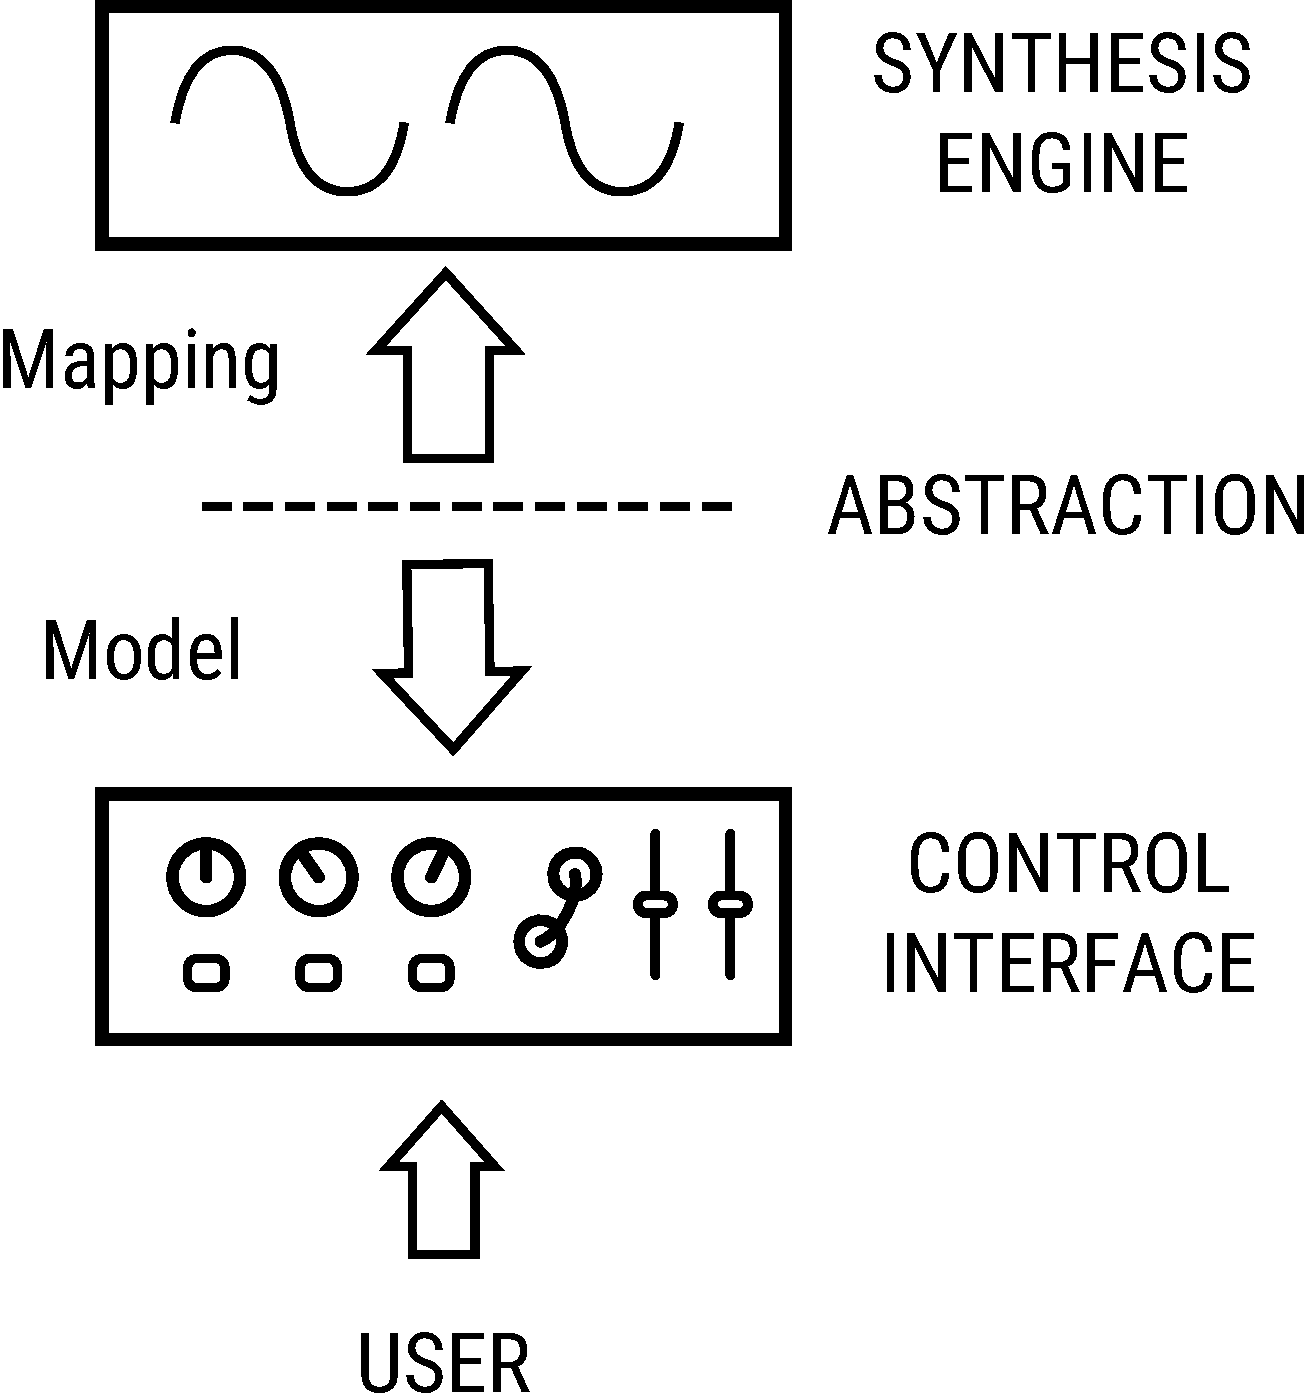
\includegraphics[width=0.4\textwidth]{figures/background/Synth Abstraction Model.pdf}
    \caption{Abstraction between the synthesis engine and control interface. A control interface on a synthesis is responsible for presenting a conceptual model of the underlying synthesis engine to a user. The parameters on the control interface are mapped back to the synthesis engine to modify audio generation.}
    \label{fig:synth_abstraction}
\end{figure}

\subsection{Synthesis Engine}
The synthesis engine is at the heart of sound generation in any synthesizer, whether it is an analog modular synth or a software audio plugin. There have been many different approaches to sound generation, and it is an active field with researchers and audio developers continuing to look for novel ways to create sounds. Sam McGuire and Nathan Van der Rest provide a good overview of some of the more popular synthesis methods in their book \textit{The Musical Art of Synthesis} \cite{mcguire2015musical}. These methods include: subtractive, sample-based, modulation (i.e. FM), additive, wavetable, granular, vector, and physically modelling. 

While the exact technique that each of these methods use may be different, there are some common components to synthesizers that exist in some form across different techniques. It is useful to take a modular perspective when thinking about different synthesizer components, similar to the \textit{unit generator} concept introduce by Max Mathews \cite{roads1980interview}, in which different components of a synthesizer are broken down into functional units (modules) that can be interconnected in various ways. We can generalize modules as all producing some output signal as well as having an optional input signal. Modules may also have some parameters that can be mapped to a control interface to enable user control. We can broadly categorize the signals that are output by modules as either audio signals or control signals. Audio signals are generated by the synthesizer and ultimately are output as a sound. Control signals are used to modulate the parameters of other modules within a synthesizer. In some synthesizers audio signals can also be treated as control signals and be used to modulate parameters of other parameters.

We can categorize modules into two different types based on the type of signal they output: 1) \textbf{audio modules}, generate or process audio signals, and 2), \textbf{control modules}, generate or process control signals. Jenkins provides an overview of some of the different synthesizer modules from the perspective of an analog synthesizer \cite{jenkins2019analog}. In analog synthesis audio signals are commonly generated by voltage-controlled oscillators (VCOs). In a VCO the frequency of the oscillator is controlled by the voltage of an input control signal. While voltages only exist in analog circuits, the concept has been extended into digital synthesizers as well, with the digital equivalent of a VCO sometimes being referred to as a digitally controlled oscillator (DCO). Other common audio modules are voltage-controlled filters (VCFs), voltage-controlled amplifiers (VCAs), and Noise Sources; filters accept audio signals as input and attenuate or boost specific frequencies, VCAs are essentially an automated volume knobs, and noise sources generate different types of noise such as white noise.

Exploring all of these methods in detail is beyond the scope of this thesis, however two methods are particularly relevant to the methods explored: subtractive synthesis and frequency modulation (FM) synthesis. 


\subsubsection{Subtractive Synthesis}
Subtractive synthesis was one of the earliest methods explored and is the sound of the famous Moog synthesizers. It has been used on thousands of records, and is still a popular method. The basic idea behind subtractive synthesis is that the starting point is a harmonically rich waveform, generated by an oscillator, which is then sent through a chain of filters and other audio effects that shape the timbre of the waveform over time. [Insert a simple block diagram of a subtractive synth]. There are several types of waveforms that are generally available on a oscillator in a subtractive synthesizer, these are shown in figure X [insert a diagram of some of the common waveforms and their harmonics]. Each waveform has a unique set of harmonics. Harmonics refer to frequencies that are present in the sound that occur at integer frequency ratios to the fundamental frequency of the sound, which is associated to the perceived pitch of that sound. Sine waves are the simplest waveforms and only contain energy at the fundamental frequency. Noise generators produce energy at all frequencies and contain no fundamental frequency and are therefore inharmonic.

Once a waveform has been generated it may be combined with other waveforms through a process called mixing. The average subtractive synthesizer has three oscillators \cite{russ2012sound} that are typically tuned to harmonically related frequencies. The next common stage in a subtractive synth signal path is an audio filter. As previously mentioned, one of the most famous synthesizer filters of all time is the Moog ladder filter \cite{moog1965voltage}, which is a resonant low pass/high-pass filter. Low pass filters allow low frequency sounds to pass through while attenuating frequencies above a certain threshold frequency, vice-versa for high-pass filters. The threshold frequency is usually controllable and can be modulated using other signals to create dynamic 'sweeping' sounds. After passing through the filter the signal passes through an amplitude gate, which acts as a volume knob that is controlled by an internal control signal envelope. The envelope 



\subsubsection{Frequency Modulation Synthesis}
FM synthesis was an another early method of synthesis that was developed during the origins of digital synthesis methods. FM synthesis engines are capable of produce a huge array of complex waveforms using a relatively simple stucture, which makes them powerful, however more conceptually challenging to understand compared to subtractive methods. The basic unit of an FM synthesizer is referred to as an operator, which generally contains a single simple sine wave oscillator and an amplitude gate controlled by an envelope generator. The simplest FM synthesizer consists of two operators that are connected together in way so that one of the operators controls the frequency of the second operator. The operator that does the modulating is referred to the \textit{modulator} and the operator that is modulated is referred to the \textit{carrier}. [Insert figure showing this arrangement.]

\subsubsection{Neural Synthesis}
One area of new development in audio synthesis is in methods that are leveraging advancements from the field of deep learning [deep learning cite], an area of audio synthesis that is explored in this thesis.  


- Pretty much just give a listing of techniques here. Potentially give a bit more of an overview of substractive vs. FM.
- Sound Synthesis and Sampling provides a thorough overview of both analog and digital synthesizers and the various methods. \cite{russ2012sound}

\subsection{Control Interface}
The control interface presents a conceptual model of the synthesizer to the user and maps this model to the underlying engine. A control interface has a set of parameters that can be altered to modify the nature of the sound being generated. A skilled sound designer is able to interact with the control interface and craft sounds to fit the needs of their creative project. This process is referred to as programming a synthesizer. A well-designed synthesizer control interfaces allow users to build up a conceptual model that allows them to easily interact with the synthesizer in a way that allows them to be expressive. 

% Not so sure about this section.
% The nature of the control interface is guided by the synthesis method being used by the engine. Synthesis methods like subtractive synthesis which involve a clear linear signal flow that starts with a complex waveform that is progressively shaped can lead to a more simple conceptual model. Moog synthesizers are examples of subtractive synthesizers that have clear control interface that maps to the synthesis engine. More complex synthesis methods such as Frequency Modulation (FM) synthesis are more challenging to create clear control maps for. Interestingly, the most commercially successful synthesizer, the Yamaha DX7, had a notoriously difficult control interface, although shipped with an extensive high-quality set of factory presets (pre-defined control interface parameter settings).

\subsection{Synthesizer Programming}
Both Carlos and Tomita excelled at patching synthesizer modules together and tuning the parameters of individual modules to create new sounds to orchestrate their performances. This process ... it's art! Blah blah blah. But also these folks are artists and virtuosos.

- Challenges with synthesizer programming UI design: \cite{seago2013new}. -- "Some, like subtractive synthesis, offer controllers which are broadly intuitive, in that changes to the parameter values produce a proportional and predictable change in the generated sound. Other methods, however, are less easily understood. FM synthesis, for example, is a synthesis method that may be viewed as essentially an exploration of a mathematical expression, but whose parameters have little to do with real-world sound production mechanisms, or with perceived attributes of sound." -- There are some other really good bits about navigating the timbre space and non-linearities.
- \cite{seago2004critical} Thus, under most current systems, the user is obliged to express directives for sound specification in system terminology, rather than in language derived from the user domain. Three types of synthesizer interfaces: parameter selection in a fixed architecture, architecture specification and configuration, and direct specification of physical characteristics of sound.
- Context on synthesizer programming \cite{jenkins2019analog}
- Russ describes the programming component intrinsically creative.
- When we talk about programming synthesizers we are referring to the task of selecting parameter settings for a synthesizer in order to achieve a desired sound
- Talk about the nature of this task. I think in that krekovic study there was something about this process? That this can be done in an exploratory way that ppl enjoy that process.
- Even so, it can still be quite a challenging task.

Programming audio synthesizers is challenging and requires a technical understanding of sound design to fully realize their expressive power. Traditional synthesizers can have over 100 parameters that affect audio generation in complex, non-linear ways. One of the most commercially successful audio synthesizers, the Yamaha DX7, was notoriously challenging to program. Allegedly nine out of ten DX7s coming into workshops for servicing still had their factory presets intact \cite{seago2004critical}.

Give an image of the complex synth UI.

% Bounce this out to another section I think. This could sit in creativity support potentially?
% \subsubsection{Neural Synthesis}
% In contrast to traditional synthesis, neural synthesizers generate audio using large-scale machine learning architectures with millions of parameters \cite{engel2017neural}. Differentiable digital signal processing \cite{engel2020ddsp} bridged the gap between traditional DSP synthesizers with the expressiveness of neural networks, exploring a harmonic model-based approach, using a more compact architecture with 100K parameters.
% One benefit of synthesized audio is that the underlying factors of variation ({\em i.e.}~the parameters) are known.

% % GANs for synthesis
% In this work, we use Generative Adversarial Networks (GANs) \cite{goodfellow2014generative} to generate new instrumental audio from a dataset of existing material. GANs have the potential to be used to generate new sounds on the fly. This would dramatically alleviate both the problem of having to pore through giant sound libraries, and the problem with having to only use one sample repeatedly. In addition, the explosion of new sounds which could potentially be produced by GANs would vastly reduce recording costs by designers of sound libraries.

% This research avenue is to a certain degree untapped: GANs have been successfully applied to the generation and manipulation of images, however, relatively little work has been focused on the audio domain. Research related to the specific work proposed here was presented by \cite{donahue2018adversarial}  and \cite{engel2018gansynth}.


\section{Creativity Support}
The field of creativity support is focused on the development of tools to enable and enhance the creative output of an individual or group, both in novice and expert users. Creativity support tools (CSTs) \cite{shneiderman2007creativity} span a wide array of application domains including visual art, textiles, cooking, and music. A central question that CSTs ask is: 
\begin{quote}
    "How can designers of programming interfaces, interactive tools, and rich social environments enable more people to be more creative more often?"
\end{quote}
 Shneiderman \cite{shneiderman2007creativity} outlines a set of design principles for developing creativity support tools which include: support exploratory search, enable collaboration, provide rich history keeping, design with low thresholds, high ceilings, and wide walls. In subsequent related work, Davis \textit{et al.} focus on the role that CSTs play in supporting novices engaging in creative tasks and the relationship that the environment plays in creativity \cite{davis2013toward}. In their work, the authors identify two types of novice users: domain novices and tool novices. Domain novices are new to both the creative domain as well as using the creativity support tool. Tool novices have experience with the creative domain, but are novices at using a particular tool. To help evaluate and promote the development of creativity support tools for novices, they also propose a theory of creativity support based on cognitive theory.

These concepts provide an important platform for beginning to develop tools to support users of synthesizers. Both types of novices described by Davis \textit{et al.} are common and serve to benefit from the development of improved methods for interacting with them; domain novices are both new to sound design / music production as well as to using a specific synthesizer, whereas a tool novices would likely have experience with sound design / music production, but would be a novice with using a specific synthesizer. 

\subsection{Music Information Retrieval}
The field of music information retrieval (MIR) is a growing research area that was born out of the need to navigate increasingly large collections of digital music. Creative MIR is a subset of the field that is focused on applying the techniques from MIR towards creative applications including music production \cite{humphrey2013brief}.

- Conversations with music producers: \cite{andersen2016conversations}

- More directly related to music the fields of MIR (creative MIR) as well as intelligent music production. - automatic mixing ref, other topics (hit up some references and expand on this)

- Overview of approaches in intelligent music production \cite{moffat2019approaches}, automatic mixing \cite{de2017ten}.

- MIR audio querying: Automatic synthesizer programming can be viewed as a retrieval task as well as an optimization problem. Viewed as a retrieval task, the problem is similar to the MIR query tasks such as Query-by-example \cite{zloof1977query}, Query-by-vocal-imitation \cite{blancas2014sound}, and query-by-beat-boxing \cite{kapur2004query}. Query problems generally build up a model of the synthesis parameter space and then return a parameter setting based on a classification that attempts to match the input with the best parameter setting.
- Visualizing sounds: \cite{wessel1979timbre} (Potentially add the George citation on visualizing sounds).

- \cite{pardo2019learning} "Learning to build natural audio production interfaces" -> Rather than force nonintuitive interactions, or remove control altogether, we reframe the controls to work within the interaction paradigms identified by research done on how audio engineers and musicians communicate auditory concepts to each other: evaluative feedback, natural language, vocal imitation, and exploration
% This could potentially be its own section
\section{Audio Representations}
- how do we represent audio digitally?
- That tutorial by that ableton author was helpful -- maybe can link to that.
- Don't go into too much depth here.
- What is a perceptually relevant method for representing audio?
- Spectral features
- STFT

% Not totally sure how to incorporate these sections?
\subsection{Learned Audio Representations}
- Representation learning \cite{bengio2013representation}
- Introduce machine learning
- self-supervised learning
- Learned audio representations
- Give a brief plug for HEAR 2021 and the need for perceptual audio representations
\section{Automatic Synthesizer Programming}
Early ASP research emerged in the late 1970s with work that focused on the use of analytic methods to estimate the parameters for frequency modulation (FM) synthesis \cite{justice1979analytic}. That work was an example of synthesizer sound matching in which a system estimates synthesizer parameters to replicate a target sound. Since then a large volume of work on synthesizer sound matching has been published and has explored a variety of synthesis techniques and algorithmic methods.
- other early methods focuses on analytic methods for programming synthesizers \cite{beauchamp1982synthesis, payne1987microcomputer, delprat1990parameter}

- Research by Benjamin Hayes on the timbre space of synths -- looks super interesting.

Since the early 90s, researchers have leveraged advances in ML to develop a deeper understanding of the synthesizer parameter space and to build more intuitive methods for interaction \cite{horner1993machine}. Recently, deep learning has been used for programming synthesizers.  Esling {\em et al.}\ \cite{esling2020flow} trained an auto-encoder network to program the \href{https://u-he.com/products/diva/}{U-He Diva} using 11K synthesized sounds with known preset values. Yee-King {\em et al.} \cite{yee2018automatic} used a recurrent network to automatically find parameters for \href{https://asb2m10.github.io/dexed/}{Dexed}, an open-source software emulation of the DX7.

- In this section an overview of the field of automatic synthesizer programming is presented. Specific emphasis is placed on the HCI aspect of the problem and an overview of various user interaction methodologies is provided here.
- Inverse synthesis, a subset of automatic synthesizer programming and a focus of this thesis, is reviewed in more detail in the following section.
- This chapter concludes with a categorization of work in automatic synthesizer programming research that has been conducted over the last 30 years.

\subsection{User Interaction}
- This is really a user interface problem. Programming synthesizers is hard!
- What are some of the different approaches that have been taken by people?
- Interactive methods (IGAs)
- Semantic search
- That interesting paper on sketching sounds visually
- Pardo look at how we can build more natural interfaces for audio production tools \cite{pardo2019learning} 

\cite{holland2013music} HCI and music interaction.

\subsubsection{Interactive Searches}
Researchers have also used Interactive Genetic Algorithms (IGAs) that allow users to interactively hear and rate potential synthesizer patches \cite{johnson1999exploring, dahlstedt2001creating, yee2016use}. In contrast to the sound matching case, the evaluation function in an IGA relies on user feedback during each iteration as opposed to measuring error between a candidate and a target. 

Reinforcement Learning and interaction \cite{scurto2021designing}

 \subsubsection{Vocal Imitations}
 It has been shown that vocal imitations are promising way to communicate sound concepts \cite{lemaitre2014effectiveness} and the VocalSketch dataset has been released to further research in this area \cite{cartwright2015vocalsketch}. Systems using vocal imitations include \cite{mcartwright2014}\cite{zhang2018visualization}. Other systems rely solely on human feedback in order to optimize towards a goal sound starting from a random selection of synthesizer patches. 
 
 \subsubsection{Semantic}
 Automatic programming using semantic sound descriptions has also been explored, and is a further methodology that has used GAs \cite{krekovic2016algorithm}.
 - Check the seago cite?
\section{Inverse Synthesis}
- inverse synthesis is the problem of estimating parameters for a synthesizer to match a target sound.
- This is the main issue that has been explored in the literature and is a big component of the research that is conducted here
 
This section provides a brief summary of the main algorithmic methodologies that have been used in previous ASP research, namely, optimization and deep learning techniques. Other methods that have been used in ASP research that are beyond the scope of this paper include  include fuzzy logic \cite{mitchell2005frequency, hamadicharef2012intelligent}, linear coding \cite{mintz2007toward}, and query approaches \cite{mcartwright2014}.

\subsection{Search vs. Modelling}
% Add something abouth the search vs. modelling approach
These two methods, the hill-climber and the LSTM++, represent two different methods for inverse synthesis; the hill-climber is a search algorithm and the LSTM++ is a modelling algorithm. Search algorithms (which include genetic algorithms) have been used extensively in the body of automatic synthesizer programming research and modelling with deep learning has been becoming more popular. Search algorithms are presented with a target sound and then begin an iterative search for the parameter settings, attempting to move closer to the target at each iteration.

\subsection{Optimization}
The optimization approach was first introduced in 1993 with Horner et al.'s work on sound matching for FM synthesis using genetic algorithms \cite{horner1993machine}. A genetic algorithm (GA) is a method for solving an optimization problem using techniques based on the principles of Darwinian evolution, and is part of a broader class of evolutionary algorithms \cite{whitley1994genetic}. In a GA, a potential solution (an individual) is represented as an array of bits. An initial set of individuals is randomly generated, and then iteratively evolved using biologically inspired processes including selection, breeding, and mutation. Individuals are ranked using an evaluation function that measures the $fitness$ of a given solution. The objective of a GA is to minimize that value (or maximize it, depending on the problem definition). The best candidates are selected for further evolution until either an optimal solution is found or a set number of evolutions has been completed.

In the case of sound matching, the \textit{fitness} of a potential solution is determined by measuring the error between a target sound and a candidate. Typically, an audio transform or audio feature extraction is performed prior to calculating \textit{fitness}. The first works on synthesizer sound matching with GAs used the Short Time Fourier Transform (STFT) in the evaluation function \cite{horner1993machine, horner1995wavetable}. Mel-frequency Cepstral Coefficients (MFCCs), an audio representation using a non-linear frequency scaling that is more relevant to human hearing, have also been used \cite{yee2008synthbot, roth2011comparison, macret2014automatic, smith2017play}. Tatar et al. introduced the use of a multi-objective GA for synthesizer sound matching that used three different methods for calculating $fitness$ values: the STFT, Fast Fourier Transform (FFT), and signal envelope \cite{tatar2016automatic}. Alternatives to GAs that have been used for sound matching include Particle Swarm Optimization (PSO) \cite{heise2009automatic} and Hill-Climbing \cite{roth2011comparison, luke2019stochastic}.

\subsection{Deep Learning}
Deep learning is subset of machine learning that utilizes artificial neural networks to learn patterns in data and make predictions based on those patterns \cite{lecun2015deep}. Deep learning architectures contain multiple layers comprised of simple non-linear modules. Through iterative training, the layers are able to extract features from raw input data and learn intricate patterns in high-dimensional data. These multi-layer architectures have enabled deep learning models to excel at complex tasks including image recognition, speech recognition, and music related tasks such as audio source separation \cite{spleeter2019}.

In the context of an ASP sound matching experiment, a deep learning model accepts an audio signal as input and predicts synthesizer parameter settings to replicate that audio signal. Audio signals are often preprocessed using audio feature extraction or an audio transform. Models are trained using a large set of example sounds generated from a synthesizer and use the parameter settings that generated a particular sound as the ground truth. During training, the error between predicted parameter settings and the actual parameter settings (the ground truth) are used to evaluate how well the model is learning and to iteratively update variables within the model to improve performance. 

Several researchers have explored the use of deep learning for ASP. Yee-King et al. reviewed several deep learning architectures for FM synthesizer sound matcing \cite{yee2018automatic}. In their work, they compared multi-layer perceptron (MLP), Long Short Term Memory (LSTM), and LSTM++ networks. Barkan et al. explored sound matching using convolutional neural networks (CNNs) \cite{barkan2019deep, barkan2019inversynth}. They framed the problem as an image classification task and used the STFT to create spectrogram images of target sounds to use as input to the CNNs. Esling et al. recently presented a novel application called $FlowSynth$ that uses a generative model based on Variational Auto-Encoders and Normalizing Flows \cite{esling2020flow}. In addition to performing well on sound matching tasks, they also showed that their approach supported novel interactions including macro-control of synthesizer parameters.

\cite{le2021improving} -- variational autoencoder. Generative approach to the synth browsing problem. Want to read this.

\cite{mitcheltree2021serumrnn} -- ensemble of models that work together to iteratively apply audio effects and select parameters for those effects to reduce the error between and input and a target. Significantly reduces the error between the input and target audio. Benefits from applying effects iteratively in a specific order. Learns which effects are most important. Provides interpretable and valuable intermediate steps. Can discover more efficient effect order sequences than a variety of baselines.

\cite{masudo2021quality} - GA based sound matching.
\section{Forty Years of Automatic Synthesizer Programming}
- organized time of all the related work. Organized based on: synthesis type and method.
- Also include a separate table for evaluation methods (maybe not totally necessary).

\begin{itemize}
	\item \cite{zloof1977query} Early example of querying sounds (need to read)
	\item \cite{justice1979analytic} Coarse parameter matching by analyzing input audio - goal was to get in the ballpark and allow for parameter tweaking afterwards. FM (Single carrier with nested modulators). Hilbert Transform. Objective evaluation.
	\item \cite{wessel1979timbre} Not specifically for synthesis methods but classic paper. This should come much earlier in this section.
	\item \cite{beauchamp1982synthesis} Matching of alto sax/cornet sounds using an analytic method for FM synthesis. Looked at spectral centroid and RMS. Objective evaluation.
	\item \cite{ashley1986knowledge} A knowledge-based approach to assistance in timbral design (need to read still)
	\item \cite{payne1987microcomputer} Hilbert Transform (time domain). Also introduced FFT version with autocorrelation on spectrum. Periodic sampled sounds, FM DX7, objective evaluation.
	\item \cite{delprat1990parameter} Parameter estimation for non-linear resynthesis methods with the help of a time-frequency analysis of natural sounds.
	\item \cite{horner1993machine} Genetic algorithms for inverse synthesis of instrumental sounds on FM synthesis engine.
	\item \cite{horner1993methods} Wavetable
	\item \cite{vuori1993parameter} Parameter estimation of non-linear physical models by simulated evolution-application to the flute model
	\item \cite{takala1993using} Using Physically-Based Models and Genetic Algorithms for Functional Composition of Sound Signals
	\item \cite{fujinaga1994genetic} Genetic algorithms as a method for granular synthesis regulation
	\item \cite{ethington1994seawave} Semantic search -- this is an good one, as far as I can tell so far this is the first semantic search for synthesizer sounds.
	\item \cite{miranda1995artificial} An artificial intelligence approach to sound design
	\item \cite{horner1995wavetable} Updated version of wavetable matching. Used multiple pitches of instrumental tones and a genetic algorithm.
	\item \cite{horner1995envelope} Envelope matching with genetic algorithms
	\item \cite{horner1996computation} Computation and memory tradeoffs with multiple wavetable interpolation
	\item \cite{horner1996piecewise} Piecewise-linear approximation of additive synthesis envelopes: a comparison of various methods
	\item \cite{cheung1996group} Group synthesis (wavetable) with genetic algorithms
	\item \cite{horner1996double} Double-modulator FM matching of instrument tones
\end{itemize}


\subsection{Synthesis Type}
An overview of synthesis type that was the focus of automatic synthesizer programming studies.

\subsubsection{FM}
\cite{justice1979analytic}\cite{beauchamp1982synthesis}\cite{payne1987microcomputer}\cite{horner1993machine}\cite{horner1996double}\cite{tan1996automated}\cite{delprat1997global}\cite{lim1999performance}\cite{tan2003automated}
\cite{mitchell2005frequency}\cite{mitchell2007evolutionary}\cite{clement2011automatic}\cite{roth2011comparison}\cite{macret2012automatic}\cite{hamadicharef2012intelligent}\cite{barkan2019deep}

\subsubsection{Non-linear}
\cite{beauchamp1982synthesis}\cite{delprat1990parameter}

\subsubsection{Wavetable / Group Synthesis}
\cite{horner1993methods}\cite{horner1995wavetable}\cite{horner1995envelope}\cite{horner1996computation}\cite{horner1996piecewise}\cite{cheung1996group}\cite{oates1997analytical}\cite{horner1998modeling}\cite{lee1999modeling}\cite{so2002wavetable}

\subsubsection{Physical Modelling}
\cite{vuori1993parameter}\cite{erkut2000extraction}\cite{liang2000recurrent}\cite{nackaerts2001parameter}\cite{riionheimo2003parameter}

\subsubsection{Granular}
\cite{fujinaga1994genetic}\cite{johnson1999exploring}

\subsubsection{Additive}
\cite{ethington1994seawave}\cite{horner1995envelope}\cite{horner1996piecewise}\cite{johnson2006timbre}\cite{mintz2007toward}

\subsubsection{Subtractive}
\cite{roth2011comparison}

\subsubsection{Generic VST}
\cite{yee2008synthbot}\cite{heise2009automatic}

\subsubsection{Other}
Noise-band \cite{chinen2007genesynth}
Concatenative \cite{stowell2010making}
Teenage Engineering OP-1 (Multiple Synthesis Engines) \cite{macret2013automatic}

\subsection{Estimation Method}
An overview of the method used to select a synthesizer parameter setting based on input.

\subsubsection{Analytic / Signal Processing}
\cite{justice1979analytic}\cite{beauchamp1982synthesis}\cite{payne1987microcomputer}\cite{ethington1994seawave}

\subsubsection{Genetic}
\cite{horner1993machine}\cite{fujinaga1994genetic}\cite{horner1995envelope}\cite{horner1995wavetable}\cite{riionheimo2003parameter}\cite{mandelis2003musical}\cite{mitchell2005frequency}\cite{mitchell2007evolutionary}
\cite{chinen2007genesynth}\cite{yee2008synthbot}\cite{roth2011comparison}\cite{macret2012automatic}\cite{hamadicharef2012intelligent}\cite{macret2013automatic}

\subsubsection{Interactive Genetic}
\cite{johnson1999exploring}

\subsubsection{Neural Network}
\cite{johnson2006timbre}\cite{roth2011comparison}\cite{zhang2018visualization}\cite{barkan2019deep}

\subsubsection{Data-driven}
\cite{roth2011comparison}\cite{mcartwright2014}

\subsubsection{Other}
Linear coding \cite{mintz2007toward}
Particle Swarm Optimization \cite{heise2009automatic}\cite{munoz2011opposition}
Regression Tree \cite{stowell2010making}
Semantic Clustering \cite{clement2011automatic}
Hill-Climber \cite{roth2011comparison}

\subsection{Unsorted}
These references have not been reviewed or sorted yet!

\cite{takala1993using}
\cite{hourdin1997sound}
\cite{horner1998nested}
\cite{wehn1998using}
\cite{garcia2001automatic}
\cite{dahlstedt2001creating}
\cite{garcia2001growing}
\cite{jehan2001perceptual}
\cite{su2002class}
\cite{le2002neural}
\cite{arfib2002strategies}
\cite{miranda2004crossroads}
\cite{schatter2005synaesthetic}
\cite{gounaropoulos2006synthesising}
\cite{lai2006automated}
\cite{mcdermott2007evolutionary}
\cite{yee2007automated}
\cite{yee2007evolving}
\cite{howard2007timbral}
\cite{mcdermott2008evolutionary}
\cite{yee2011automatic}
\cite{mitchell2012automated}
\cite{povscic2013controlling}
\cite{seago2013new}
\cite{krekovic2014intelligent}
\cite{macret2014automatic}
\cite{itoyama2014parameter}
\cite{huang2014active}
\cite{fasciani2016tsam}
\cite{krekovic2016algorithm}
\cite{tatar2016automatic}
\cite{yee2016use}
\cite{smith2017play}
\cite{yee2018automatic}
\cite{luke2019stochastic}

	\graphicspath{{./}{./figures/}{./figures/spiegelib/}}

\chapter{Inverse Synthesis}

\section{Goals}
\begin{enumerate}
    \item Main contributions: spiegelib software, initial experiments using Dexed.
    \item Goal is to explore some of the main recent approaches to inverse synthesis and compare them in the task of finding parameters to match a target sound
    \item Expand on the experimental research -- provide a bit more background on the specific methods that we are trying to emulate. Specifically: the genetic algorithm approaches and the deep learning approaches.
    \item Identify some of the challenges faced with this approach: rendering from VSTs is slow. Recent techniques SPSA could allow for VSTs to be inserted directly into the pipeline. Leads us to an area for future work: torchsynth
\end{enumerate}

Will have given a bit of a history by this point in the background -- something similar to Brecht's paper, but for automatic synthesizer programming. Here we want to focus on the main techniques that we want to use.

\section{Plan}
\begin{enumerate}
    \item This chapter explores the inverse synthesis problem. This is based on work I completed under the supervision of my supervisors and was published at AES ...
    \item Contributes SpiegeLib software and demonstrates the steps of conducting an inverse synthesis experiment through some experiments.
    \item Software in Inverse Synthesis -- overview the available software. Give some motivation based on reproducible research. Maybe add a figure that outlines the experimental process and how each of the library components fit together to help with this.
    \item SpiegeLib
    \item Experiment -- Go into more detail on the specific algorithms and methods that are being used here. Can give some code detail as well if that would be helpful.
    \item Evaluation -- How are the results evaluated and list the results
    \item Conclusion
\end{enumerate}

\section{Introduction}
The use of sound synthesizers in the fields of music composition, production, and performance is widespread, but the task of programming a synthesizer is complex and requires a thorough understanding of technical details. It is not uncommon for a software synthesizer to have 30+ parameters displayed on a user interface (UI) and labelled using technical names \cite{rasmussen2018evaluating}. Manually programming sounds using such a large set of parameters is a daunting task. Synthesizer programming is further complicated by the fact that modifications to parameters are often not intuitively reflected in the end sonic result. This disconnect can be disruptive to the creative process. Automatic synthesizer programming (ASP) is the field of research focused on addressing these challenges in programming synthesizers.

 Early ASP research emerged in the late 1970s with work that focused on the use of analytic methods to estimate the parameters for frequency modulation (FM) synthesis \cite{justice1979analytic}. That work was an example of synthesizer sound matching in which a system estimates synthesizer parameters to replicate a target sound. Since then a large volume of work on synthesizer sound matching has been published and has explored a variety of synthesis techniques and algorithmic methods. One popular approach is the use of evolutionary algorithms \cite{horner1993machine, mitchell2007evolutionary, yee2007evolving, yee2008synthbot, heise2009automatic, roth2011comparison, tatar2016automatic, smith2017play}. More recently, deep learning techniques have been explored \cite{yee2018automatic, barkan2019inversynth, esling2020flow}. Other methods that have been studied include semantic descriptions \cite{ethington1994seawave, johnson2006timbre, krekovic2016algorithm}, interactive methods \cite{johnson1999exploring, dahlstedt2001creating, yee2016use}, and sound matching with vocal imitations \cite{mcartwright2014, zhang2018visualization}.
 
 A recent user study conducted by Krekovi{\'c} et al. confirmed the desire among synthesizer users for improved means of working with their synthesizers \cite{krekovic2019insights}. 
 %Users identified approaches they felt would be particularly beneficial, which included automatic sound matching and improvements to user interface design. 
 While recent research has produced promising results, automatically programming a modern software synthesizer still presents challenges. Current evolutionary techniques face issues including time complexity \cite{tatar2016automatic}, while recent deep learning approaches have challenges in consistently producing accurate reproductions \cite{yee2018automatic}. The desires expressed by the users in Krekovi{\'c} et al.'s study, coupled with the need for further research and improvement noted in the existing body of work, point to the need for further development in ASP.
 
 The work presented here attempts to continue this development, and promote collaboration and reproducibility in ASP research through the introduction of \mintinline{python}{spiegelib}, an open-source library written in the Python programming language. Vandewalle et al. argue that reproducibility in computational science research increases the impact of a work and they provide a framework for evaluating the quality of reproducibility \cite{vandewalle2009reproducible}. The aim of \mintinline{python}{spiegelib} is to provide a platform for researchers of automatic synthesizer programming to develop, test, and share implementations in a way that promotes reproducibility at the highest level. \mintinline{python}{spiegelib} stands for Synthesizer Programming with Intelligent Exploration, Generation, and Evaluation Library. The name \mintinline{python}{spiegelib} was chosen to pay homage to Laurie Spiegel, an early pioneer in electronic music composition. Laurie Spiegel is known for utilizing synthesizers and software to automate certain aspects of the music composition process. Her philosophy for using technology in music serves as a motivation for the \mintinline{python}{spiegelib} software library: "I automate whatever can be automated to be freer to focus on those aspects of music that can't be automated. The challenge is to figure out which is which." \cite{hinkle2006women}
 
 The remainder of this paper is structured as follows: Section \ref{sec:2} presents a survey of related work to provide background for the algorithmic techniques included in \mintinline{python}{spiegelib} as well as an overview of available open-access ASP software, Section \ref{sec:3} provides an overview of the \mintinline{python}{spiegelib} software library. An example case illustrating the use of \mintinline{python}{spiegelib} in a research context is presented in Section \ref{sec:4}.

\section{Related Work}\label{sec:2}
This section provides a brief summary of the main algorithmic methodologies that have been used in previous ASP research, namely, optimization and deep learning techniques. Other methods that have been used in ASP research that are beyond the scope of this paper include  include fuzzy logic \cite{mitchell2005frequency, hamadicharef2012intelligent}, linear coding \cite{mintz2007toward}, and query approaches \cite{mcartwright2014}. An  informal survey of open-access software that supports reproducibility is also included at the end of the section.

\subsection{Optimization}
The optimization approach was first introduced in 1993 with Horner et al.'s work on sound matching for FM synthesis using genetic algorithms \cite{horner1993machine}. A genetic algorithm (GA) is a method for solving an optimization problem using techniques based on the principles of Darwinian evolution, and is part of a broader class of evolutionary algorithms \cite{whitley1994genetic}. In a GA, a potential solution (an individual) is represented as an array of bits. An initial set of individuals is randomly generated, and then iteratively evolved using biologically inspired processes including selection, breeding, and mutation. Individuals are ranked using an evaluation function that measures the $fitness$ of a given solution. The objective of a GA is to minimize that value (or maximize it, depending on the problem definition). The best candidates are selected for further evolution until either an optimal solution is found or a set number of evolutions has been completed.

In the case of sound matching, the \textit{fitness} of a potential solution is determined by measuring the error between a target sound and a candidate. Typically, an audio transform or audio feature extraction is performed prior to calculating \textit{fitness}. The first works on synthesizer sound matching with GAs used the Short Time Fourier Transform (STFT) in the evaluation function \cite{horner1993machine, horner1995wavetable}. Mel-frequency Cepstral Coefficients (MFCCs), an audio representation using a non-linear frequency scaling that is more relevant to human hearing, have also been used \cite{yee2008synthbot, roth2011comparison, macret2014automatic, smith2017play}. Tatar et al. introduced the use of a multi-objective GA for synthesizer sound matching that used three different methods for calculating $fitness$ values: the STFT, Fast Fourier Transform (FFT), and signal envelope \cite{tatar2016automatic}. Alternatives to GAs that have been used for sound matching include Particle Swarm Optimization (PSO) \cite{heise2009automatic} and Hill-Climbing \cite{roth2011comparison, luke2019stochastic}.

Researchers have also used Interactive Genetic Algorithms (IGAs) that allow users to interactively hear and rate potential synthesizer patches \cite{johnson1999exploring, dahlstedt2001creating, yee2016use}. In contrast to the sound matching case, the evaluation function in an IGA relies on user feedback during each iteration as opposed to measuring error between a candidate and a target. 

Automatic programming using semantic sound descriptions has also been explored, and is a further methodology that has used GAs \cite{krekovic2016algorithm}.

\subsection{Deep Learning}
Deep learning is subset of machine learning that utilizes artificial neural networks to learn patterns in data and make predictions based on those patterns \cite{lecun2015deep}. Deep learning architectures contain multiple layers comprised of simple non-linear modules. Through iterative training, the layers are able to extract features from raw input data and learn intricate patterns in high-dimensional data. These multi-layer architectures have enabled deep learning models to excel at complex tasks including image recognition, speech recognition, and music related tasks such as audio source separation \cite{spleeter2019}.

In the context of an ASP sound matching experiment, a deep learning model accepts an audio signal as input and predicts synthesizer parameter settings to replicate that audio signal. Audio signals are often preprocessed using audio feature extraction or an audio transform. Models are trained using a large set of example sounds generated from a synthesizer and use the parameter settings that generated a particular sound as the ground truth. During training, the error between predicted parameter settings and the actual parameter settings (the ground truth) are used to evaluate how well the model is learning and to iteratively update variables within the model to improve performance. 

Several researchers have explored the use of deep learning for ASP. Yee-King et al. reviewed several deep learning architectures for FM synthesizer sound matcing [11]. In their work, they compared multi-layer perceptron (MLP), Long Short Term Memory (LSTM), and LSTM++ networks. Barkan et al. explored sound matching using convolutional neural networks (CNNs) [12]. They framed the problem as an image classification task and used the STFT to create spectrogram images of target sounds to use as input to the CNNs. Esling et al. recently presented a novel application called $FlowSynth$ that uses a generative model based on Variational Auto-Encoders and Normalizing Flows [13]. In addition to performing well on sound matching tasks, they also showed that their approach supported novel interactions including macro-control of synthesizer parameters.

\subsection{Software in ASP Research}
 In Vandewalle et al.'s paper on reproducibility in computational sciences, they advocate providing other researchers with "all the information (code, data, schemes, etc.) that was used to produce the presented results"\cite{vandewalle2009reproducible}. Several authors of ASP research have started to make their work open-access with source code available online. 
 
 Martin Roth and Matthew Yee-King developed $JVstHost$, a Java-based Virtural Studio Technology (VST) plugin host that was published by Matthew Yee-King \cite{yee2011automatic} and was a component of $SynthBot$ \cite{yee2008synthbot}. However, the code for $SynthBot$ itself was not released. Matthew Yee-King also shared the source code for $EvoSynth$, an application for interactive synthesizer patch exploration \cite{yee2016use}. A version of $EvoSynth$ is hosted online allowing for immediate experimentation\footnote{\url{http://www.yeeking.net/evosynth/}}. Krekovi{\'c} et al. released source code for their $MightyKnob$ system \cite{krekovic2016algorithm}. Esling et al. released open-source code and a Max4Live\footnote{\url{https://www.ableton.com/en/live/max-for-live/}} application for $FlowSynth$ \cite{esling2020flow}. Yee-King et al. recently took initial steps towards a software framework for ASP research with the release of source code that provides functionality for generating research datasets and a set of algorithms for parameter estimation \cite{yee2018automatic}. Along with that work they released the $RenderMan$\footnote{\url{https://github.com/fedden/RenderMan}} library for programmatically interacting with VST synthesizers using the Python programming language.
 
 \mintinline{python}{spiegelib} builds upon this work with the goal of supporting and encouraging reproducibility within the ASP research community. \mintinline{python}{spiegelib} is inspired by the steps that Yee-King et al. took towards creating a software library for ASP research and extends that work with the inclusion of: an object-oriented API, base classes for customization, more robust evolutionary techniques, basic subjective evaluation, complete documentation, and packaging and delivery. It provides a framework for authors to share implementations in an open-access way that allows other researchers to quickly recreate results using a clearly documented set of freely-available tools.
 
% Updated table if necassary
%\begin{table*}[t]
%\centering\small
%\begin{threeparttable}
%	\caption{Algorithms currently implemented as classes in \mintinline{python}{spiegelib}}
%	\label{table:spiegel_algorithms}
%	\begin{tabular}{|c|c|c|c|}
%	\hline
%	\multicolumn{4}{|c|}{\textbf{Algorithms in \mintinline{python}{spiegelib}}} \\
%	\hline
%	\hline
%	\textbf{Feature Extraction} & \textbf{Deep Learning Estimators} & \textbf{Optimization Estimators} & \textbf{Evaluation} \\
%	\hline
%	FFT 		& MLP \cite{yee2018automatic} 		& Basic GA  	& MFCC Evaluation \\
%	STFT 		& LSTM \cite{yee2018automatic} 		& NSGA III \cite{tatar2016automatic} & Basic Subjective \\\cline{3-4}
%	MFCC		& LSTM++ \cite{yee2018automatic} \\
%	Spectral\tnote{1}	& Conv6 \cite{barkan2019inversynth} \\\cline{1-2}
%	\end{tabular}
%	\begin{tablenotes}[para, flushleft]
%			\footnotesize
%			\item[1] Spectral bandwidth, centroid, contrast, flatness, and rolloff.
%	\end{tablenotes}
%\end{threeparttable}
%\end{table*}

\begin{table*}[t]
\centering\small
\begin{threeparttable}
	\caption{Algorithms currently implemented as classes in \mintinline{python}{spiegelib}}
	\label{table:spiegel_algorithms}
	\begin{tabular}{|c|c|c|}
	\hline
	\multicolumn{3}{|c|}{\textbf{Algorithms in \mintinline{python}{spiegelib}}} \\
	\hline
	\hline
	\textbf{Feature Extraction} & \textbf{Deep Learning Estimators} & \textbf{Optimization Estimators} \\
	\hline
	FFT 		& MLP \cite{yee2018automatic} 		& Basic GA   			\\
	STFT 		& LSTM \cite{yee2018automatic} 		& NSGA III \cite{tatar2016automatic}				\\\cline{3-3}
	MFCC		& LSTM++ \cite{yee2018automatic} 	& \textbf{Objective Evaluation} 	\\\cline{3-3}
	Spectral\tnote{1}	& Conv6 \cite{barkan2019inversynth} 	& MFCC Evaluation 		\\
	\hline
	\end{tabular}
	\begin{tablenotes}[para, flushleft]
			\footnotesize
			\item[1] Spectral bandwidth, centroid, contrast, flatness, and rolloff.
	\end{tablenotes}
\end{threeparttable}
\end{table*}
 
\section{Design of SpiegeLib}\label{sec:3}
\mintinline{python}{spiegelib} is designed to be as extensible as possible to allow researchers to develop and test new implementations of components for conducting ASP research. Base classes with functionality for interacting with software synthesizers, audio feature extraction, parameter estimation, and evaluation provide an API to support development of custom implementations that will work with other components of the library. A number of utility classes are also provided for handling audio signals, generating datasets, and running experiments.

 \mintinline{python}{spiegelib} is written in the Python programming language and utilizes Python packages common in research including \mintinline{python}{numpy}, \mintinline{python}{scipy}, \mintinline{python}{tensorflow}, and \mintinline{python}{librosa}. \mintinline{python}{spiegelib} itself is a python package and is available through the Python Package Index (PyPI) with pip\footnote{\url{https://pypi.org/}}. All dependencies, except for \mintinline{python}{librenderman}, are python packages available through the PyPI and will be automatically installed by pip. For more information on installation, system requirements, and detailed library documentation, please refer to the  online documentation.\footnote{\url{https://spiegelib.github.io/spiegelib/}}
 
 A summary of the currently implemented algorithms is shown in table \ref{table:spiegel_algorithms}. A brief overview of these components and the main classes and functionalities of \mintinline{python}{spiegelib} is provided in the following sections.
 
\subsection{AudioBuffer}
The \mintinline{python}{AudioBuffer} class is used to pass audio signal signals throughout the library. It holds an array of audio samples and sample rate information. Methods of the \mintinline{python}{AudioBuffer} class provide functionality for loading audio from a variety of file formats, resampling, normalizing, time segmenting, plotting spectrograms, and saving audio as WAV files.

\subsection{Synthesizers}
The \mintinline{python}{SynthBase} class is an abstract base class that provides an interface for creating programmatic interactions with software synthesizers. \mintinline{python}{SynthBase} stores information and contains methods required for interaction with other components in \mintinline{python}{spiegelib}, including getting parameter lists, setting and getting patch configurations, overriding/freezing parameters, triggering audio rendering using MIDI notes, getting audio samples as \mintinline{python}{AudioBuffer}s, and requesting randomized patch settings. All patch settings are stored as a list of parameter tuples which contain the parameter number and parameter value. All parameter values are expected to be floating point numbers in the range [0.0, 1.0]. No requirement is made on how underlying synthesis engines are implemented, however, inheriting classes must provide parameter descriptions in a class attribute during construction and must provide implementations for four abstract class methods related to loading patches, randomizing patches, rendering audio, and returning an \mintinline{python}{AudioBuffer} of rendered audio.

%
% \mintinline{python}{load_patch()}, \mintinline{python}{randomize_patch()}, \mintinline{python}{render_patch()}, and \mintinline{python}{get_audio()}.

\mintinline{python}{SynthVST} is an implementation of \mintinline{python}{SynthBase} and provides an interface for interacting with VST synthesizers. \mintinline{python}{SynthVST} is a wrapper for the $RenderMan$ Python library developed by Leon Fedden in conjunction with research by Yee-King et al. \cite{yee2018automatic}.

\subsection{Audio Feature Extraction}
The abstract base class \mintinline{python}{FeaturesBase} provides an interface for audio feature extraction tasks. 
The \mintinline{python}{getFeatures()} abstract method must be overridden in inheriting classes and is where feature extraction algorithms are run.  \mintinline{python}{FeatureBase} also includes functionality for normalizing results from feature extraction. By default, data is normalized by removing the mean and scaling to unit variance. Settings for normalization can be saved from a set of data, reloaded, and applied to new feature extraction results to ensure that normalization is carried out using the same parameters. Currently, implemented feature extraction classes utilize the \mintinline{python}{librosa} library \cite{mcfee2015librosa} and include Mel Frequency Cepstral Coefficients (\mintinline{python}{MFCC}), Short Time Fourier Transform (\mintinline{python}{STFT}), Fast Fourier Transform (\mintinline{python}{FFT}), and a set of time summarized spectral features (\mintinline{python}{SpectralSummarized}).

\subsection{Estimators}
All parameter estimation classes implement the \mintinline{python}{EstimatorBase} abstract base class. \mintinline{python}{EstimatorBase} is a minimal base class with one abstract method, \mintinline{python}{predict()}, that has an optional input argument. Implementations of estimators are split into deep learning approaches and other approaches including evolutionary algorithms.  The included algorithms do not represent a comprehensive set of methods for ASP research but are meant to cover common methods informed by previous work. Six estimators are currently implemented and the authors plan to add 5 more in the near future: a hill climbing optimizer \cite{yee2018automatic}, a particle swarm optimizer \cite{heise2009automatic}, additional configurations of 2D CNNs \cite{barkan2019inversynth}, a 1D CNN for raw audio input \cite{barkan2019inversynth}, and a recent generative approach \cite{esling2020flow}. The authors hope that other researchers will add their new algorithms to the library as well.

\subsubsection{Deep Learning Estimators}
All deep learning models are implementations of the \mintinline{python}{TFEstimatorBase} abstract base class which utilizes the \mintinline{python}{tensorflow}\footnote{\url{https://www.tensorflow.org}} and \mintinline{python}{keras}\footnote{\url{https://www.tensorflow.org/guide/keras}} machine learning libraries. \mintinline{python}{TFEstimatorBase} implements \mintinline{python}{EstimatorBase} and provides wrapper functions for setting up data for training and validation, training models, running predictions, and saving and loading model weights. While these methods are designed to help in handling of data typical to a synthesizer parameter estimation problem, all methods for a \mintinline{python}{tf.keras.Model} can be accessed directly from the \mintinline{python}{model} class member. Classes that inherit from \mintinline{python}{TFEstimatorBase} define models in an implementation of the \mintinline{python}{buildModel()} method which is automatically called during construction in the base class. This allows new models to be quickly designed, switched out, and compared with minimal effort.

Currently, implementations for a Multi-Layer Perceptron (\mintinline{python}{MLP}), Long Short Term Memory (\mintinline{python}{LSTM}), Bi-directional Long Short Term Memory with Highway Layers (\mintinline{python}{HwyBLSTM}), and a convolution network with 6-layers (\mintinline{python}{Conv6}) are included. An example code listing of sound matching using a trained LSTM model is shown in figure \ref{fig:lstm_code}.

To save training and validation progress, the \mintinline{python}{TFEpochLogger} class can be passed in as a callback during model training. \mintinline{python}{TFEpochLogger} stores training accuracy and loss, and validation accuracy and loss over training epochs in a dictionary object which can be plotted after training.

%Example code listing
\begin{figure}[t]
\centering
\caption{Example of \mintinline{python}{spiegelib} performing a sound match from a target WAV file on a VST synthesizer. A pre-trained LSTM deep learning model is used with MFCC input.}
\footnotesize
\begin{minted}{python}
import spiegelib as spgl
import spiegelib.estimator.TFEstimatorBase

# Load VST and set parameters from JSON file
synth = spgl.synth.SynthVST('./Dexed.vst')
synth.load_state('./dexed_simple_fm.json')

# MFCC Audio Feature Extractor
ftrs = spgl.features.MFCC(normalize=True)

# Load saved normalization parameters
ftrs.load_normalizers('./normalizers.pkl')

# Load LSTM model from saved model file
lstm = TFEstimatorBase.load('./fm_lstm.h5')

matcher = spgl.SoundMatch(synth, lstm, ftrs)

target = spgl.AudioBuffer('./target.wav')
output = matcher.match(target)
output.save('./lstm_predicted_audio.wav')
\end{minted}
\label{fig:lstm_code}
\end{figure} 

\subsubsection{Optimization Estimators}
Two optimization estimators are currently implemented and utilize the DEAP python library \cite{fortin2012deap}. A basic GA (\mintinline{python}{BasicGA}) is included as well as a multi-objective non-dominated sorting genetic algorithm III (\mintinline{python}{NSGA3}). Both GAs require feature extraction objects, or a list of feature extraction objects in the case of the multi-objective algorithm, which are used in the GA evaluation function. 

\subsection{Datasets}
The \mintinline{python}{DatasetGenerator} class provides functionality for creating datasets of audio samples, feature vectors, and associated parameter settings from a synthesizer. An implementation of \mintinline{python}{SynthBase} and \mintinline{python}{FeaturesBase} are passed in as arguments to the \mintinline{python}{DatasetGenerator} constructor. To generate a dataset, random patches for the synthesizer are created and feature extraction is performed on the resulting audio. In this way, datasets for training and validating deep learning models, as well as datasets for evaluating sound matching experiments can be automatically generated. 
%The term contrived in the context of ASP research refers to the use of audio samples produced by the synthesizer being studied as a target for sound matching \cite{justice1979analytic}. The benefit of using a contrived sound for evaluation is that it minimizes the uncertainty regarding whether the synthesizer in question is capable of producing the target sound. 
External datasets can also be used within \mintinline{python}{spiegelib} and the \mintinline{python}{AudioBuffer} class provides support for loading folders of audio samples for processing.

\subsection{Evaluation}
Objective evaluation of results can be carried out by measuring error between audio samples. \mintinline{python}{EvaluationBase} is an abstract base class for calculating evaluation metrics on a set of target and prediction data. A list of target values and lists of predictions for each target are passed into the constructor. \mintinline{python}{EvaluationBase} provides functionality for calculating statistics on results, saving results as a JSON file, plotting results in histograms, and calculating metrics including mean absolute error, mean squared error, euclidian distance, and manhattan distance. Inheriting classes must implement the \mintinline{python}{evaluate_target()} method which is called for each target and associated estimations and is expected to return a dictionary of metrics for each estimation. The \mintinline{python}{MFCCEval} class implements \mintinline{python}{EvaluationBase} and calculates metrics on MFCC vectors for targets and estimations.

Functionality for conducting subjective evaluation of results is provided in the \mintinline{python}{BasicSubjective} class. This class accepts a set of audio files and runs a locally hosted server that generates a simple web interface for listening to and ranking audio files in terms of similarity or preference. For sound matching experiments, audio targets can be passed in along with a set of predictions for each target, and a sound similarity test will be generated with options for randomizing the ordering of targets and predictions. Results can then be saved as a JSON file.

\section{Example Case}\label{sec:4}
\subsection{Dexed: FM Sound Matching}
To illustrate the use of \mintinline{python}{spiegelib} in the context of an ASP sound matching experiment, we present an example study that compares six different parameter estimators acting on $Dexed$\footnote{\url{https://asb2m10.github.io/dexed/}}, a VST software emulation of the Yamaha DX7 FM synthesizer. The methodology used for this experiment is modelled after Yee-King et al.'s study on deep learning for automatic synthesizer programming \cite{yee2018automatic}, but with a simplified synthesizer configuration and a unique set of estimators. In alignment with Vandewalle et al.'s criteria for reproducible research, implementation details, code, and datasets are all available on the \mintinline{python}{spiegelib} online documentation.\footnote{\url{https://spiegelib.github.io/spiegelib/examples/fm_sound_match.html}}

The first step is defining the synthesizer setup and creating data for training deep learning models. $Dexed$ has 155 parameters controllable through the \mintinline{python}{SynthVST} class. A subset of nine of these parameters were used in this experiment to turn $Dexed$ into a simple two-oscillator FM synthesizer. The \mintinline{python}{SynthVST} class provides methods for overriding and freezing parameters as well as saving and loading parameter settings as JSON files.

The \mintinline{python}{DatasetGenerator} class was then used to create datasets for deep learning training. All deep learning models, except for the CNN, used a 13-band MFCC calculated with a frame size of 2048 samples and a hop size of 1024 samples. The input of the CNN was the magnitude spectrum from a STFT, calculated using an FFT with 512 bins and a hop size of 256 samples. Using an instance of \mintinline{python}{DatasetGenerator}, 50,000 training examples and 10,000 validation examples were generated by randomly sampling the nine parameters from $Dexed$. Resulting feature vectors were normalized by removing the mean and scaling to unit variance using methods within the \mintinline{python}{FeatureBase} base class. Datasets and settings for normalization were then stored as NumPy\footnote{\url{https://numpy.org/}} files for later use.

All deep learning models are defined in classes within \mintinline{python}{spiegelib} and all inherit from \mintinline{python}{TFEstimatorBase}. Models were trained using an $Adam$ optimizer \cite{kingma2014adam}, batch sizes of 64, and used an early stopping callback which halted training if validation loss was stagnant for 10 epochs to prevent overfitting. Logging of training and validation progress was recorded using the \mintinline{python}{TFEpochLogger} class. The loss function in all models measure the RMS error between ground truth parameter settings and prediction parameter settings. 
%Plots of training and validation accuracy and loss for the LSTM++ model are shown in figure \ref{fig:lstm_bi_train}. Trained models are then saved for future use.

%\begin{figure}[]
%\begin{center}
%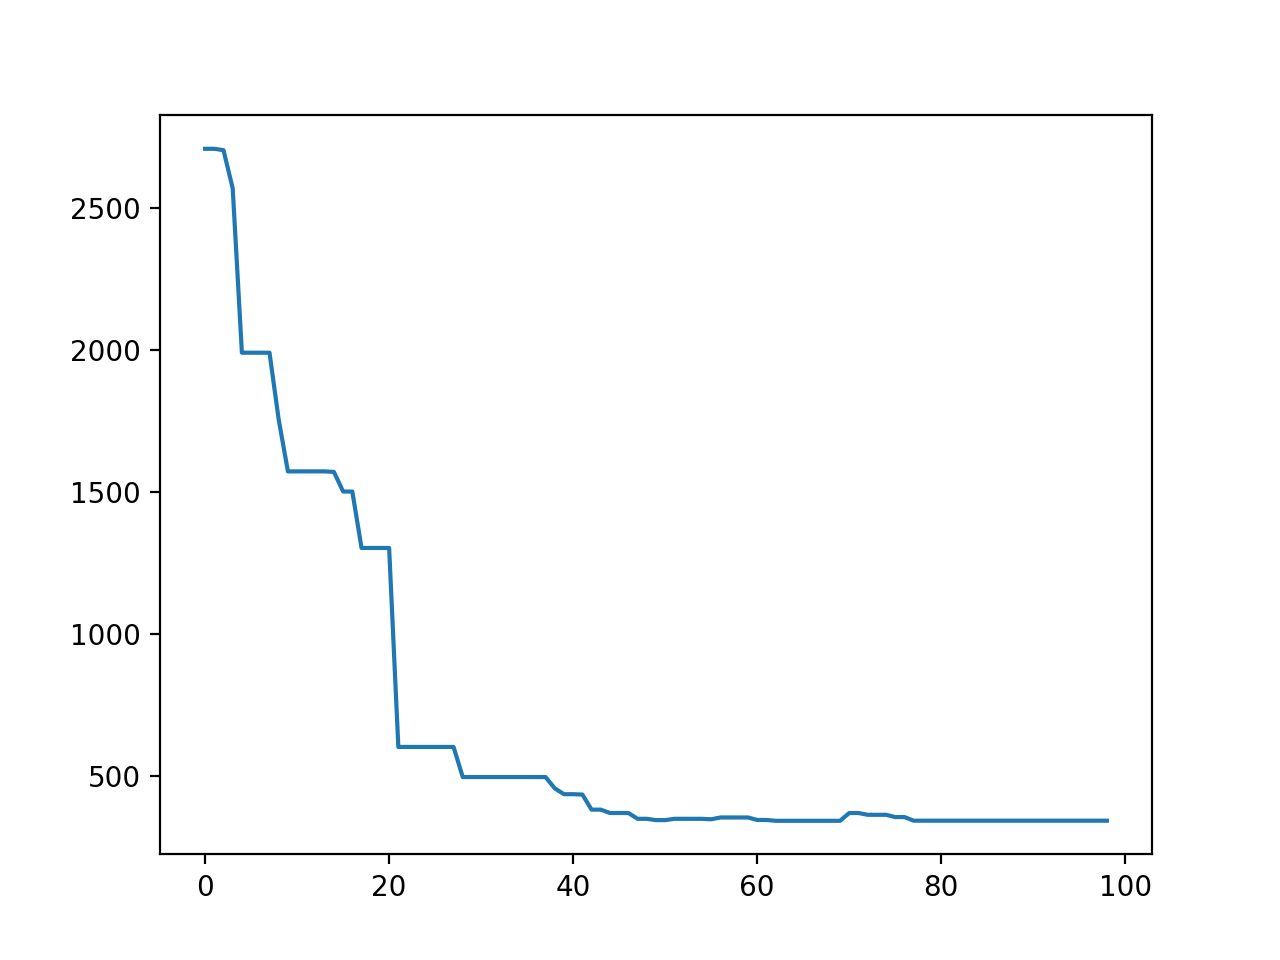
\includegraphics[width=0.95\columnwidth]{nsga_target_15_FFT.png}
%\caption{Minimum FFT MAE in the population at each generation to target sound 15 for NSGA III estimator.}
%\label{fig:nsga_fitness}
%\end{center}
%\end{figure}

Two GAs were used: a basic single-objective GA (\mintinline{python}{BasicGA}) and a multi-objective NSGA III (\mintinline{python}{NSGA3}). Evaluation functions for the GAs use audio feature extraction and measure the mean absolute error (MAE) between the target and individuals to calculate $fitness$. The \mintinline{python}{BasicGA} used a 13-band MFCC in the evaluation function and the \mintinline{python}{NSGA3} used three different extractors: a 13-band MFCC, STFT, and five spectral features. Both genetic algorithms were run for 100 generations for each sound target.

%\begin{figure}[t]
%\begin{center}
%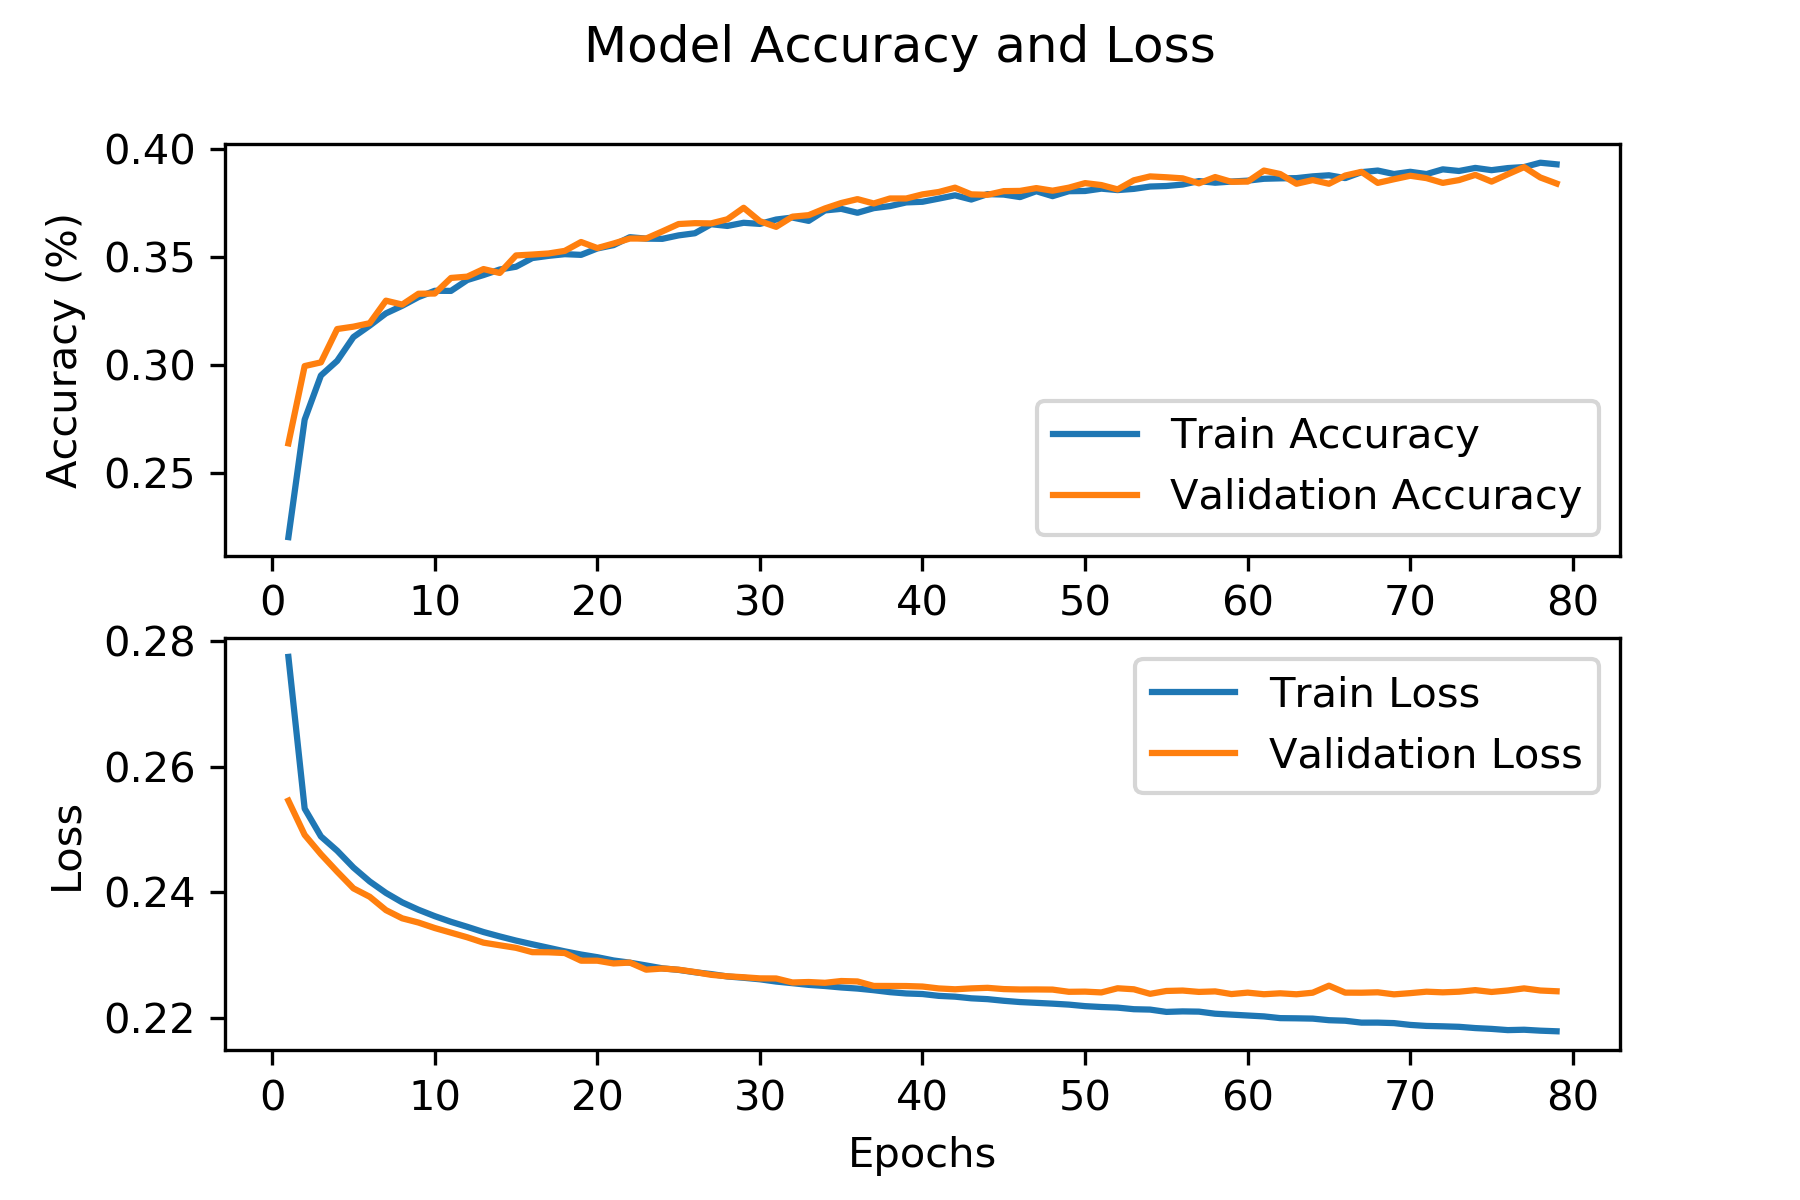
\includegraphics[width=0.95\columnwidth]{blstm_training.png}
%\caption{Traing and validation accuracy and loss over epochs for LSTM++ model training.}
%\label{fig:lstm_bi_train}
%\end{center}
%\end{figure}

An evaluation dataset containing 25 random sounds from the same nine-parameter $Dexed$ configuration was generated using the \mintinline{python}{DatasetGenerator} class. All estimators were run on each one of the 25 target sounds using the \mintinline{python}{SoundMatch} class. \mintinline{python}{SoundMatch} is a functional class that uses an estimator to predict synthesizer parameter settings for an implementation of \mintinline{python}{SynthBase} in order to match a target sound. This resulted in a set of audio files generated from $Dexed$ using the estimated parameters from each estimator run on each of the 25 target sounds. These audio files were then used for objective evaluation.

\begin{table}[t]
\centering
\caption{Results from sound matching evaluation}
\label{tbl:sound_match_eval}
\begin{threeparttable}
\begin{tabular}{l|cccc}
\toprule
$Method$ & $Mean$ & $SD$ & $Min$ & $Max$ \\
\midrule
$MLP$ & 8.55 & 6.77 & 1.92 & 34.12 \\
$CNN$ & 7.88 & 4.26 & 2.68 & 20.89 \\
$LSTM$ & 6.12 & 3.76 & 1.20 & 19.36 \\
$LSTM++$ & 4.91 & 6.50 & 2.12 & 21.51 \\
$GA$ & 2.25 & 2.58 & 0.70 & 11.17 \\
$NSGA III$ & \textbf{0.81} & \textbf{0.89} & \textbf{0.001} & \textbf{3.06} \\
\bottomrule
\end{tabular}
\begin{tablenotes}[para, flushleft]
\footnotesize
\item Values shown are calculated from the mean absolute error (MAE) calculated during MFCC evaluation. Smaller MAE values indicate more similar matches. The NSGA III estimator received the best scores, which are shown in bold font.
\end{tablenotes}
\end{threeparttable}
%\vspace{5mm}
\end{table}

\begin{figure}[t]
\begin{center}
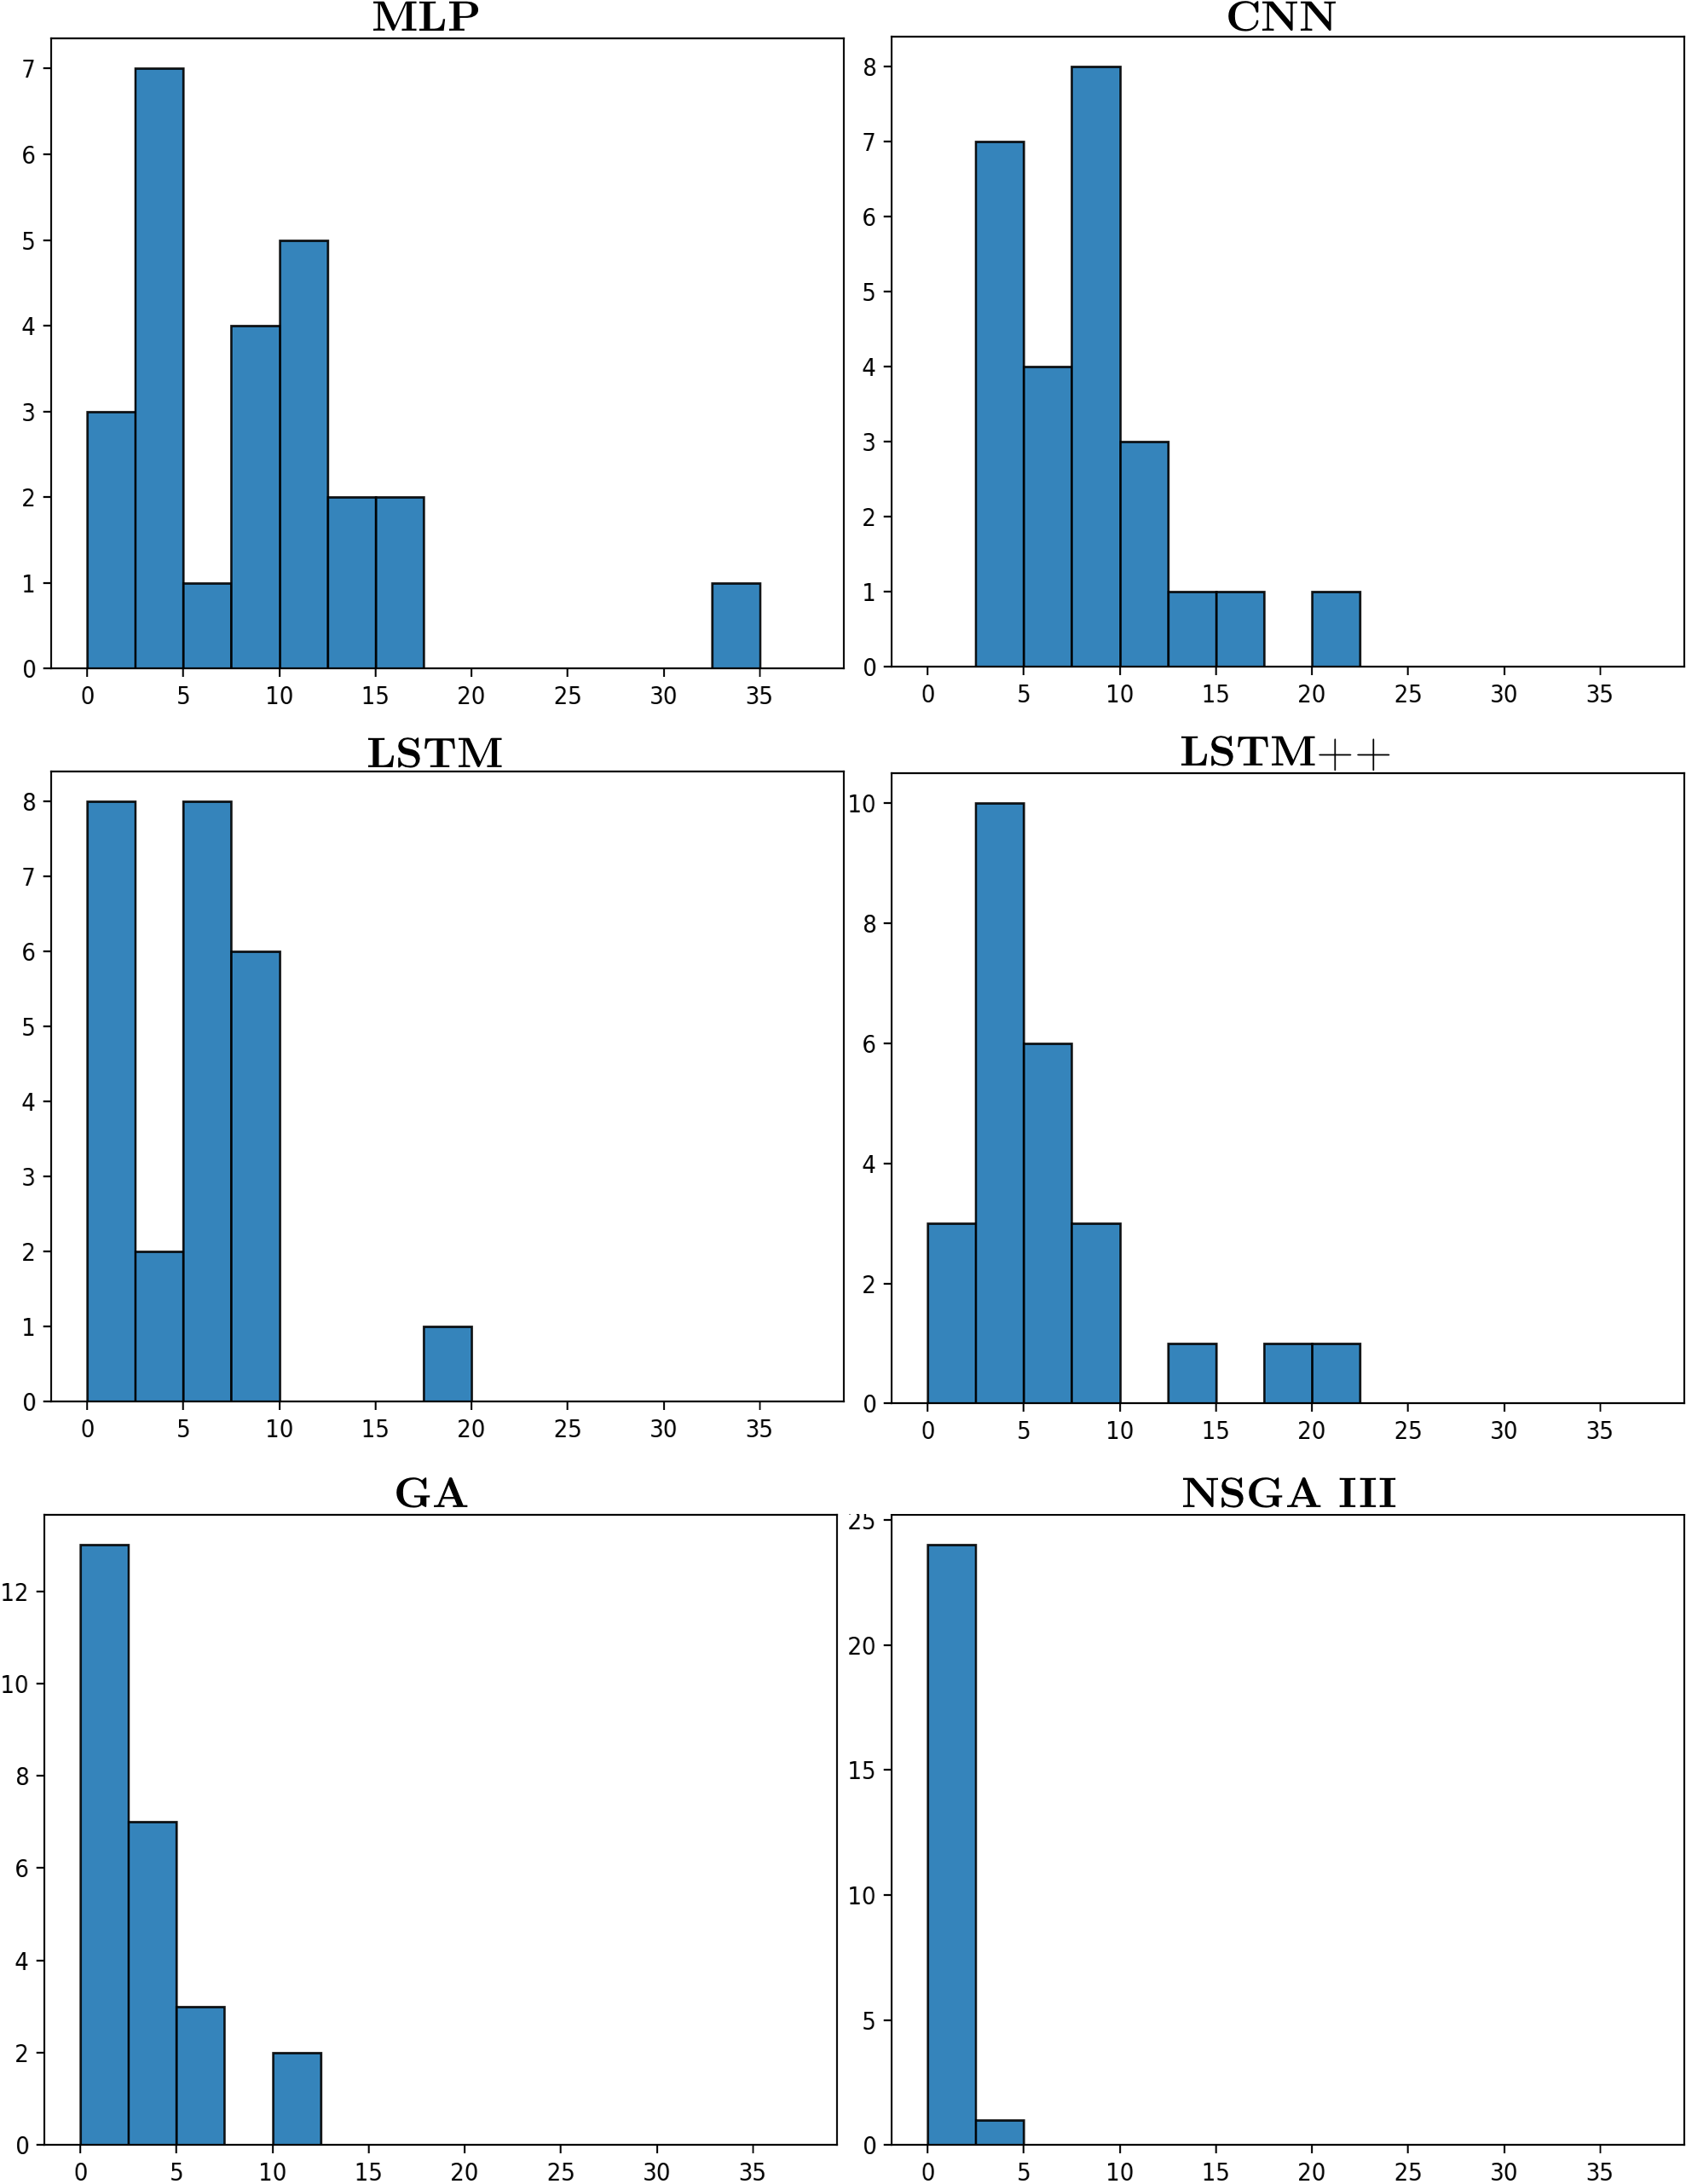
\includegraphics[width=0.75\textwidth]{hist_group_v3.png}
\caption{Histogram shows the MAE values resulting from MFCC evaluation run on a set of 25 sound targets for all estimators. Lower MAE values indicate a closer sound match.}
\label{fig:group_hist}
\end{center}
\end{figure}

\begin{figure}[t]
\begin{center}
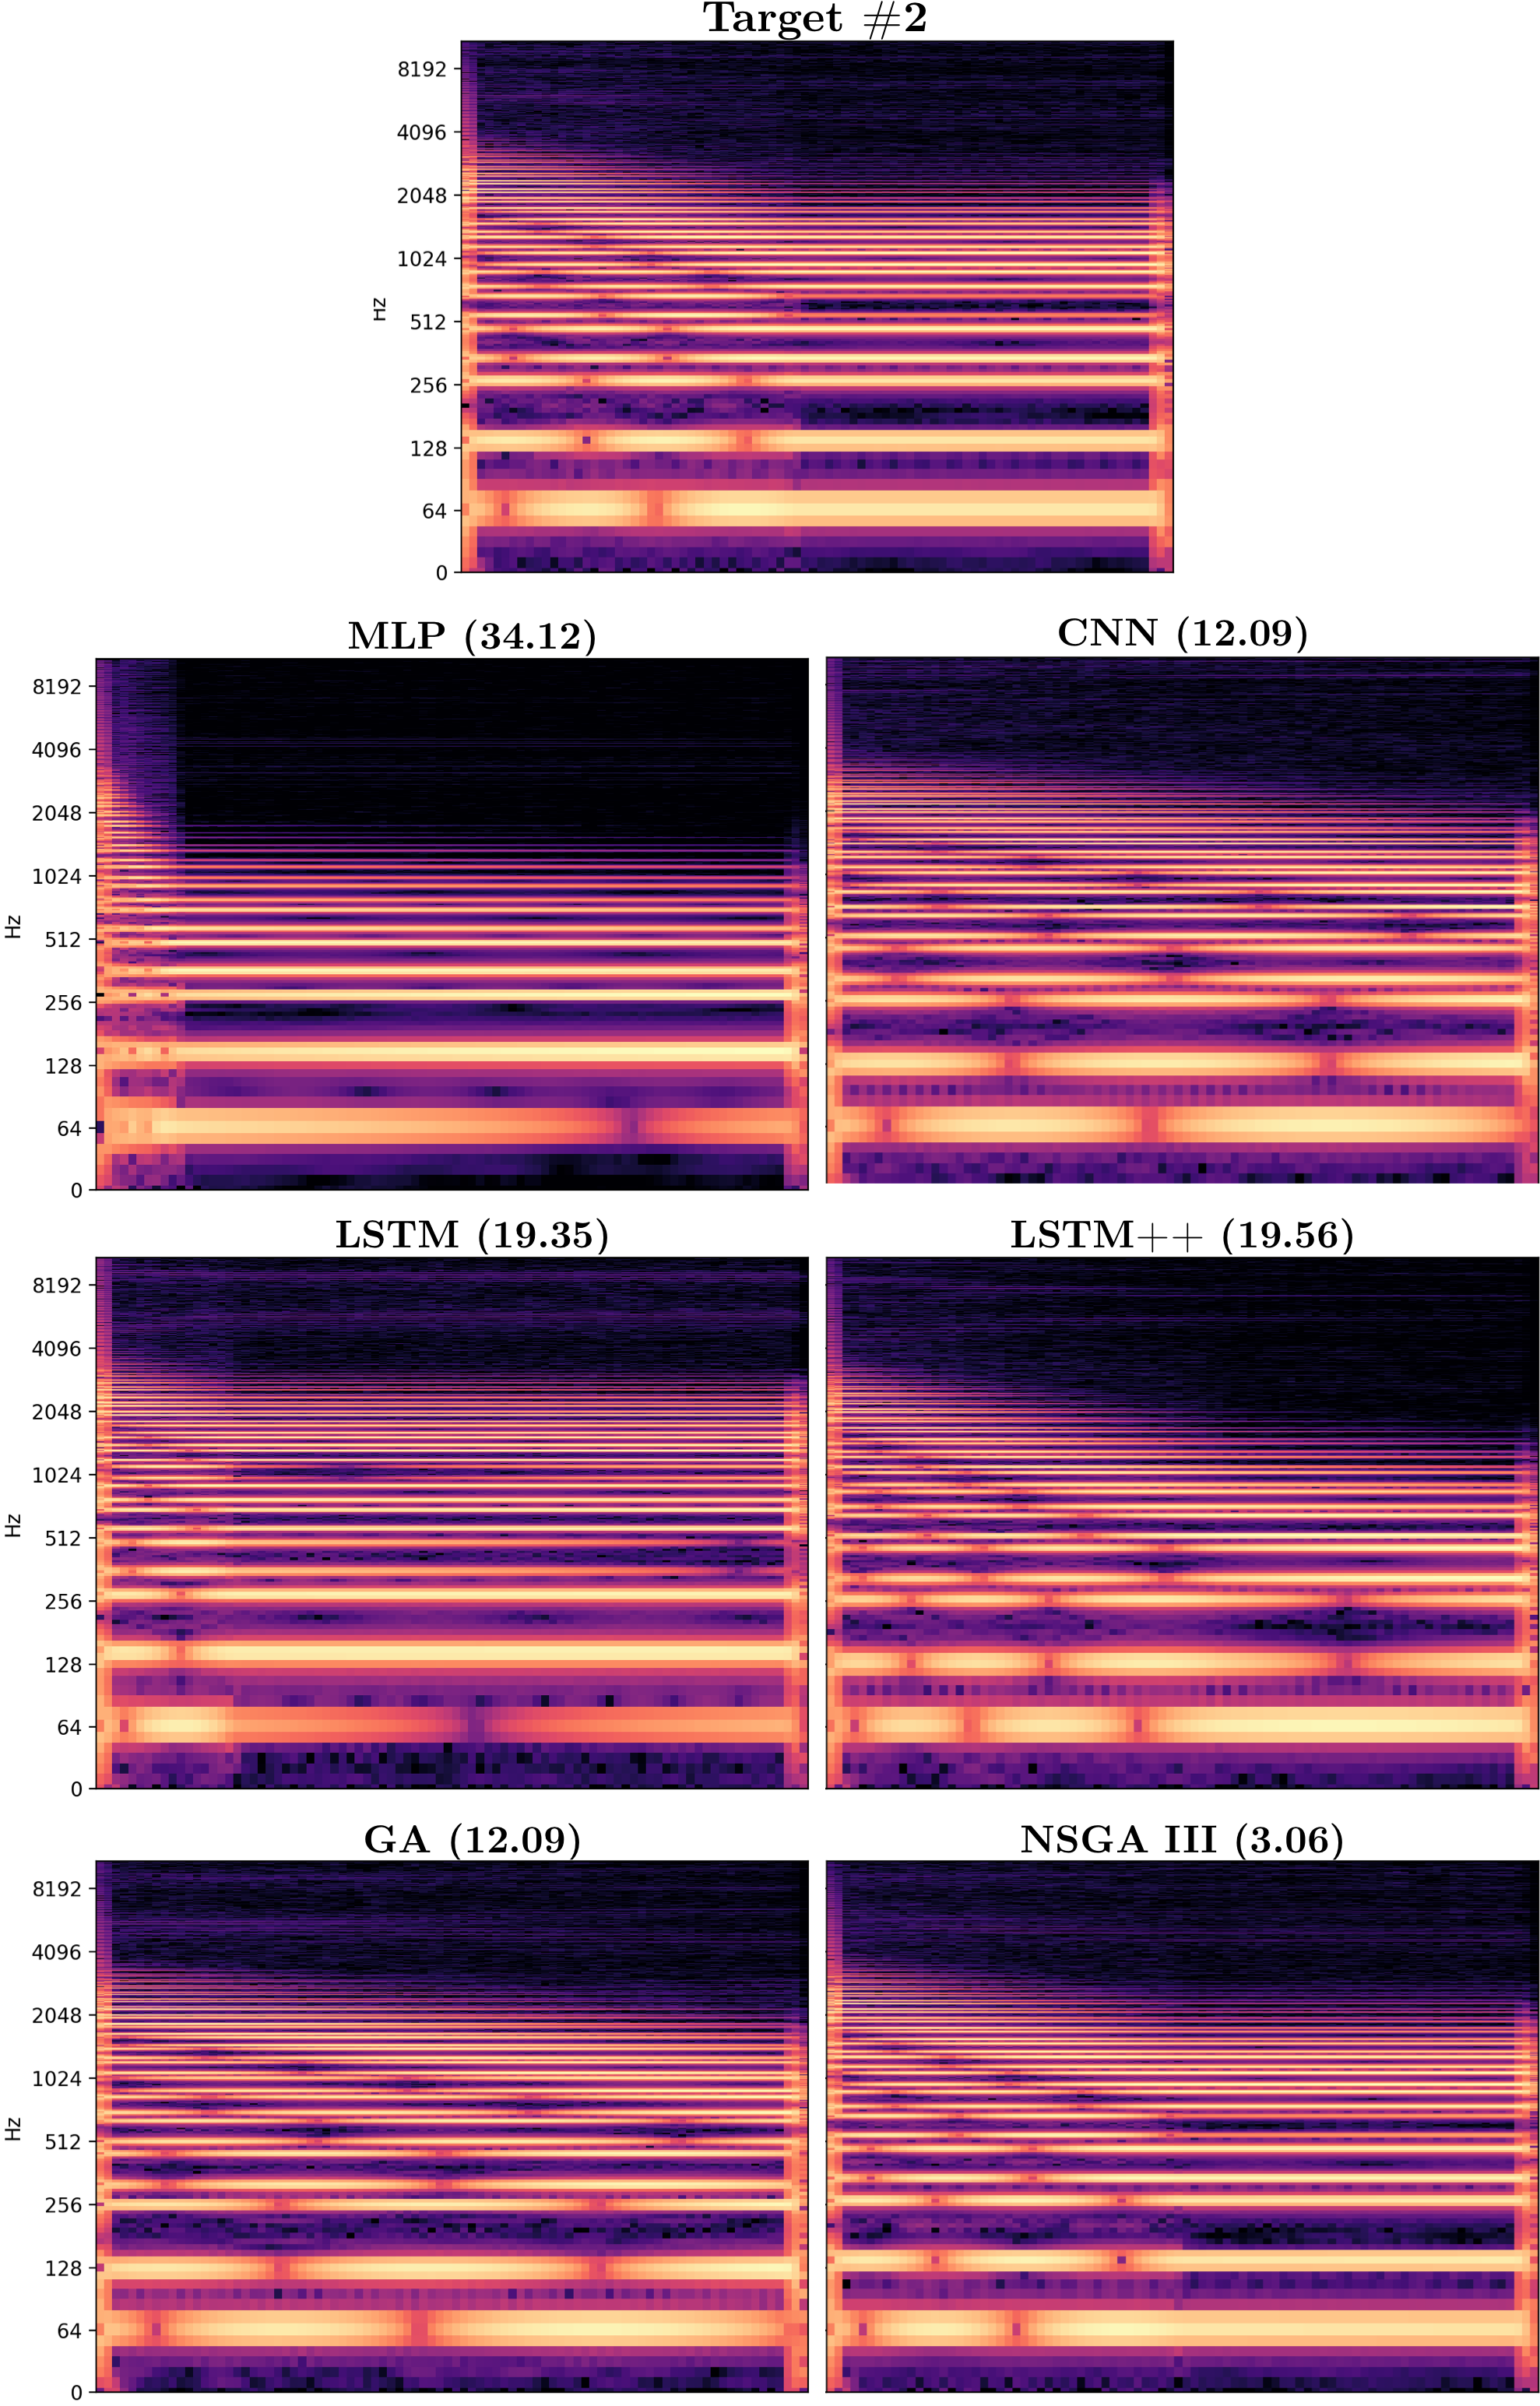
\includegraphics[width=0.75\textwidth]{spect_group_v1.png}
\caption{Spectrogram plots of a target sound and sound match predictions made by each estimator. The value next to the estimator name is the MAE value from MFCC evaluation for that prediction (lower MAE values indicate a closer match).}
\label{fig:group_spect}
\end{center}
\end{figure}

To evaluate to the resulting predictions the \mintinline{python}{MFCCEval} class was used, which calculates error and distance metrics on MFCCs of a target and prediction. Results for mean absolute error (MAE) which have been summarized using mean, standard deviation, minimum, and maximum, are shown for each estimator in table \ref{tbl:sound_match_eval}. Both GAs performed better than the deep learning approaches with the NSGA III having the best overall score. For deep learning approaches, the LSTM++ model achieved the best mean score. Histograms of the the MAE were also plotted for each estimator using the \mintinline{python}{plot_hist()} method in \mintinline{python}{EvaluationBase}. Histograms of the MAE for all predictions made by all estimators are shown in figure \ref{fig:group_hist}. Spectrograms of one target sound and sound match predictions made by each of the estimators for that target are shown in figure \ref{fig:group_spect}. For this particular target, spectrograms reveal that while the frequency and distribution of the harmonics was relatively close for each estimation, all estimators except for the NSGA III struggled with matching the temporal envelope of the spectrum.

% If we have time!!
%\subsection{Tunefish: Interactive Genetic}

\section{Future Work and Conclusion}
Development of \mintinline{python}{spiegelib} is ongoing and a number of expansions to the current library are planned. First, we would like to continue to expand the number of estimators available and plan on integrating the following: a hill climbing optimizer \cite{yee2018automatic}, a particle swarm optimizer \cite{heise2009automatic}, more 2D CNN configurations \cite{barkan2019inversynth}, a 1D CNN for raw audio input \cite{barkan2019inversynth}, and a generative approach \cite{esling2020flow}.  Second, we would like to expand on the type of interactions available such as automatic programming from vocal imitations \cite{mcartwright2014} and interactive methods. 
%Third, we would like to integrate more sophisticated subjective evaluation tools such as creating links to setup tests using the Web Audio Evaluation Tool \cite{waet2015}. Third, we would like to contribute to the $RenderMan$ library that is used in this work in order to extend support to Windows users and distribute the library via PyPI so the entire \mintinline{python}{spiegelib} library can be installed in one command. 
Finally, we would like to encourage developers and researchers from the automatic synthesizer programming community to contribute to \mintinline{python}{spiegelib}. Information on contributing is available online.\footnote{\url{https://spiegelib.github.io/spiegelib/contributing.html}} 

This work has introduced \mintinline{python}{spiegelib}, an open-source automatic synthesizer programming library. \mintinline{python}{spiegelib} is an object-oriented library that was designed with the goal of supporting development, collaboration, and reproducibility in the field. The library includes implementations of classes for conducting ASP research. These classes contain functionality for interacting with VST synthesizers, extracting audio features, creating datasets, estimating synthesizer parameters, and evaluating results. Six implementations of deep learning and evolutionary parameter estimation techniques based on previous work are included, with more planned. An example case of an automatic synthesizer sound matching study using the library was shown. This example case, along with the supporting code and data available online showcases how \mintinline{python}{spiegelib} can be used to support reproducible research.

	\graphicspath{{./}{./figures/}{./figures/neural/}}

\chapter{Neural Synthesis}

\section{Introduction}
Music producers and sound-effect artists require the frequent use of audio samples, for example to simulate a snare drum hit or a gunshot sound. The process of arduously searching through multi-gigabyte sound libraries for the right sound is extremely time-consuming; and its alternative, of creating a brand new sound using audio synthesizers, requires a formidable technical background. To compound this difficulty, in a track or action scene containing hundreds of snare drum hits or gunshots, the process of using the same (or same few) samples repeatedly can lead to a canned effect. What is required is a method for simultaneously trimming down the size of a library while simultaneously (and in some sense paradoxically) increasing sound variability.

In this work, we use Generative Adversarial Networks (GANs) \cite{goodfellow2014generative} to generate new instrumental audio from a dataset of existing material. GANs have the potential to be used to generate new sounds on the fly. This would dramatically alleviate both the problem of having to pore through giant sound libraries, and the problem with having to only use one sample repeatedly. In addition, the explosion of new sounds which could potentially be produced by GANs would vastly reduce recording costs by designers of sound libraries.

This research avenue is to a certain degree untapped: GANs have been successfully applied to the generation and manipulation of images, however, relatively little work has been focused on the audio domain. Research related to the specific work proposed here was presented by \cite{donahue2018adversarial}  and \cite{engel2018gansynth}.

Through the work in our project, we implemented a GAN following the approach of \cite{donahue2018adversarial}, and trained it using instrumental audio samples from the freely available NSynth dataset\footnote{\url{https://magenta.tensorflow.org/datasets/nsynth}}, published by \cite{nsynth2017} from Google's Magenta research lab. The NSynth dataset contains over 300k four second long audio samples of labelled musical instruments, including flute, brass, string, and other instrument sounds. We explored several variations to the baseline model proposed by \cite{donahue2018adversarial}, including a perceptually motivated model using spectrograms. Our results show that the time-domain based model performed the best for our instrumental synthesis task, and one of the major findings of our project show that significant improvements were made by adding dropout to generator model.

\section{Problem Definition}
The specific problem that was being tackled was the generation of one second of audio in the style of a specific, solo musical instrument. The focus of our initial experiments was to train a GAN to generate one second of a flute sound at a specific pitch. We followed the general approach of \cite{donahue2018adversarial} in implementing a WaveGAN, a GAN the produce time-domain audio signals. Among the features implemented in the WaveGAN are a DCGAN architecture, a Wasserstein loss function, phase shuffling to make training easier for the generator and inception and nearest-neighbor scores for evaluation. Of these features, the only one we had no time to implement was the inception score. 

Additionally, we developed an idea on our own for a variation on the WaveGan model that uses the Mel-Spectrogram. This reframes the audio generation problem back into the image generation domain by using a time series of mel-scale frequency bands to create a spectrogram image. Donahue et al. experimented with a similar approach using the Short-time Fourier Transform (STFT). The STFT is a linear frequency audio representation. However, humans perceive frequency in a logarithmic scale. Mel-Spectrograms represent audio in the frequency domain using the mel-frequency scale, which is a logarithmic based scale based on human auditory perception. While MFCCs are typically not invertible, there exist approximations allowing for transform to the time-domain, with which we experimented and compared results to the time-domain based GAN that we also developed. This approach is somewhat analogous to the SpecGAN implemented by Donahue et al.

Additionally, we attempted some architecture variations, in an attempt to eliminate checkerboard artifacts and improve overall model training. Based our these findings we trained GANs using a selection of other instruments.

\section{Related Work, Background Information}

The concept of Generative Adversarial Nets was introduced in 2014 by \cite{goodfellow2014generative}. A tremendous amount of research has been devoted to the topic of improving GANs. An architecture which has been shown to work well in practice for generating images is the Deep Convolution Neural Network (\cite{radford2015unsupervised}).

One problematic feature of the DCGAN, however, is its propensity for generating checkerboard artifacts, as visible in Figure \ref{checkerboard}. These are believed to be an effect of the transpose-convolution layers in the DCGAN generator. One possible solution, proposed by \cite{Odena2016DeconvolutionAC} is the use of resize or upsampling layers.

\begin{figure}
\centering
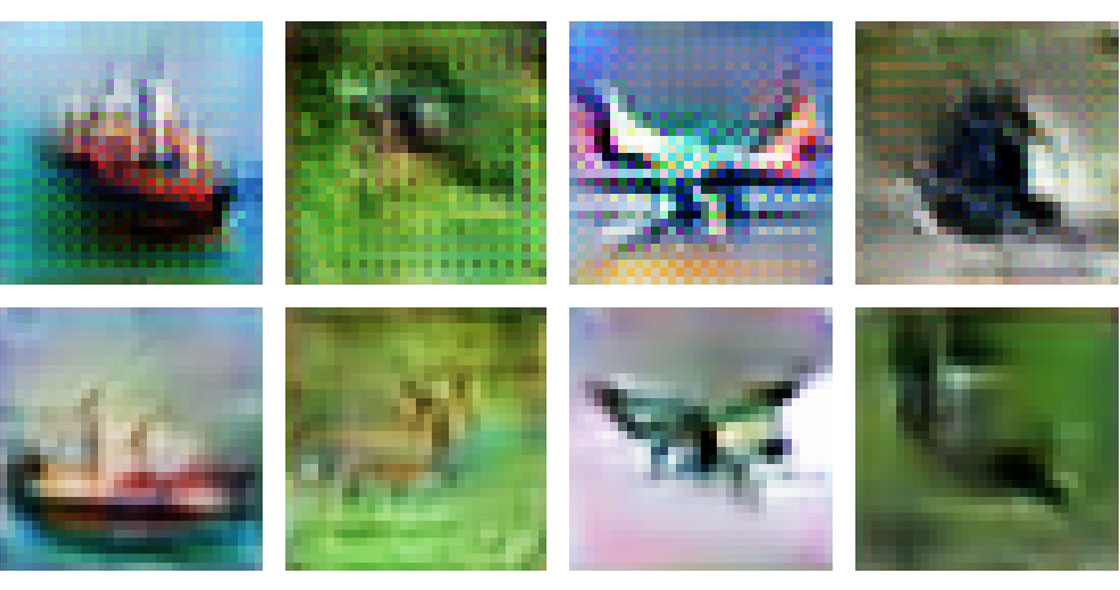
\includegraphics[width=0.8\textwidth]{checkerboard.jpg}
\caption{We see examples of the checkerboard effect commonly associated with GANs which use the transpose convolution. Credit: \cite{Odena2016DeconvolutionAC}.}
\end{figure}\label{checkerboard}

An important technical advancement in the theory of GANs was to relax the topology on the probability distributions from the strong to weak-* topologies (for more information, see Appendix A). This gave rise to the Wasserstein GAN, as proposed by \cite{arjovsky2017wasserstein}. The Lipschitz constraint was naively implemented in the original by weight clipping. Later, \cite{gulrajani2017improved} considered a more sophisticated solution, the WGAN-GP (Wasserstein GAN - Gradient Penalty), which relied on insights from the field of optimal transport (see for example \cite{villani_2009}).

The foregoing technology was developed to solve the problem of image generation. Donahue et al. (\cite{donahue2018adversarial}) have applied the WGAN-GP to the problem of audio generation. Their application was done along two different lines. The first, and most obvious method was to apply standard GAN image generation techniques to audio spectrograms (the SpecGAN). The second method was to slightly reframe the DCGAN architecture to accommodate 1-dimensional time series data (waveforms) instead of 2-dimensional images (the WaveGAN). They found slightly better success in the latter approach.

\section{Methods}
We first attempted to recreate the baseline WaveGAN algorithm proposed by \cite{donahue2018adversarial}, which was a simple modification to DCGAN. The DCGAN model, which generated images in the style of the MNIST dataset, was developed first, and then modified to accommodate one second long audio samples instead of images. This modification involved flattening the DCGAN layers to support one-dimensional signals instead of two-dimensional images. The original DCGAN model supported 64x64 pixel images, which corresponds to a 4096 length signal when flattened. To support audio signals one second long at a sampling rate of 16kHz, an additional convolution layer was added to bring to the final output of the generator up to 16384. The discriminator model from DCGAN was modified in a similar manner. Further details on this architecture are provided in Appendix B.

\subsection{WGAN-GP}
Building on this baseline DCGAN architecture, the WGAN-GP was implemented by modifying the loss functions and implementing a gradient penalty that is added to the discriminator loss. The baseline DCGAN model was trained using the approach proposed by \cite{goodfellow2014generative}, which seeks to solve the following dual minimization problem:
\begin{equation*}\label{eqn:goodfellow_minimization}
    \min_{G}\left(\max_{D}\left(\sum_{x\text{ real}}\log(D(x))-\sum_{z\text{ latent}}\log(D(G(z)))\right)\right)
\end{equation*}

where $N$ samples are taken i.i.d. from the space of real waveforms, and the latent space, respectively. The generator $G$ and the discriminator $D$ are allowed to be arbitrary neural networks, in this case the modified DCGAN networks. Note that this is not precisely the form of loss derived in Appendix A; it has been slightly modified to avoid vanishing gradients.

In the case of the WGAN, the loss is modified to:
\begin{equation*}
    \min_{G}\left(\max_{D}\left(\sum_{x\text{ real}}D(x)-\sum_{z\text{ latent}}D(G(z))\right)\right)
\end{equation*}
where now $D$ is required to have gradient norm $\leq 1$. This condition is achieved by applying a gradient penalty on convex combinations pairs of points from the real, and generated datasets.

\subsection{Architecture Variations}\label{sec:variation}
\subsubsection{Mitigating Checkerboard Artifacts}
A number of variations to the the model architecture were explored in attempt to improve the quality of audio generated. The checkerboard artifacts identified by \cite{Odena2016DeconvolutionAC} present additional challenges in the realm of audio signals compared to images. \cite{donahue2018adversarial} note that in the case of images, the discriminator might be able to use these artifacts as a way of identifying fakes images, whereas in audio signals repeating patterns are common in pitched signals which could introduce additional challenges for the discriminator in distinguishing between intentional repetitions and artifacts. Finding ways to mitigate these artifacts is beneficial as they result in unpleasant distortions in the final audio signals.

The first approach that we applied to remedy this issue was to apply resizing layers, which was suggested by \cite{Odena2016DeconvolutionAC}. The resizing layers precede the convolution layers in the generator and take over the role of upsampling the signal, which was previously handled using transpose operations within the convolution. One the of the effects that these resizing layers have is mitigating the effect of aliasing that can occur during upsampling using transpose convoluation layers. Four different methods for resizing were tested: basic upsampling, nearest neighbour interpolation, linear interpolation, and cubic interpolation.

The second approach that we explored to mitigate the adverse effect checkerboard artifacts on training was phase shuffling, proposed by \cite{donahue2018adversarial}. Phase shuffling is applied after each convolution layer in the discriminator and applies a small random time shift by $-N$ to $N$ samples to the signal, where $N$ is a hyperparameter set to control the amount of shifting applied. This process makes the discriminator's job more challenging by forcing it to handle phase invariance.

\subsubsection{Batch Normalization}
Batch normalization can be applied after each convolution layer to normalize results prior to the next layer. This was applied to all layers in both the generator and discriminator in the original DCGAN model. Removing batch normalization in the discriminator was a necessity due to the addition of the gradient penalty in the WGAN-GP, as described by \cite{gulrajani2017improved}. In the case of the generator, \cite{donahue2018adversarial} experimented with also removing batch normalization from the generator. We also experiment with removing batch normalization from the generator model.

\subsubsection{Dropout}
Dropout is a regularization method used in deep learning networks to combat overfitting \cite{srivastava2014dropout}. When using dropout, a percentage of nodes from an output layer are randomly left out, which has been found to improve training. A dropout of 30\% was included in the discriminator from the original DCGAN model and was left in throughout experiments. We experimented with adding 50\% dropout to the generator model.

\subsubsection{Kernel Size}
Adjusting the kernel size in the discriminator affects to number of parameters in the model and therefore the capacity of the model. The original image DCGAN model used a kernel size of (5x5) which translates to a kernel size of 25 in the audio DCGAN discriminator. To reduce the complexity of the discriminator in our initial experiments we used a smaller kernel size of 5, which allowed for quicker training time for the initial model variations. Later experiments modified this kernel size and experimented with increasing the size up to 15 and 25. The kernel size in the generator was kept at 25 throughout all experiments.

\subsection{MelGAN}\label{sec:methods_melgan}
Using a spectrogram representation of audio reframes the audio GAN problem back into the image domain. \cite{donahue2018adversarial} experimented with this approach with their proposed SpecGAN by producing spectrogram images of size (128x128) using the Short-Time Fourier Transform (STFT). One issue with the STFT is that it produces linear-spaced frequency-bins and humans perceive pitch and frequency on a logarithmic scale. The mel-frequency scale is a perceptually informed scaling based on human hearing and techniques exist to map the results from the STFT onto this frequency scale \cite{stevens1940relation}. One issue with using spectrograms for audio generation is that they are not typically invertible due the loss of phase information during spectrogram creation. In order to perform signal reconstruction in this case, phase can be estimated using the Griffin-Lim algorithm \cite{griffin1984signal}, which is the approach we took here.

%\begin{figure}
%\centering
%\includegraphics[width=0.48\textwidth]{MelSpectroGram %transform.png}
%\caption{Conversion of an audio time series signal to a mel-spectrogram. Mel-spectrogram is produced using a Short-Time Fourier Transform with size 2056, hop length of 128. Resulting linear frequency bins are mapped to 128 mel-frequency bins. The x-axis of the mel-spectrogram represents time and the y-axis frequency in the mel-scale, the magnitude of each value in the mel-spectrogram represents the energy at that frequency and time.}
%\end{figure}\label{fig:melspectrogram}

To explore the benefit of using a perceptually motivated spectrogram for audio generation, we experiment with using mel-spectrograms in combination with the WGAN-GP, we call the resulting model MelGAN. The time-series training data was converted to the time-frequency domain using the STFT with an FFT of size 2056 and a hop-length of 128 samples. The resulting linear frequency bins were then mapped to 128 mel-frequency bins. The amplitude was then converted to a logarithmic scale, which is a more perceptual relevant measurement of amplitude, and then scaled to a range between 0 and 1. This resulted in a set of mel-spectrogram images of size (128x128). The flattened DCGAN architecture was converted back to a model that could handle images. %Figure \ref{fig:melspectrogram} shows an example of a time-domain audio signal and its resulting mel-spectrogram.


\section{Experiments}
All experiments were conducted using the NSynth dataset \cite{nsynth2017}. Initial experiments comparing the DCGAN to the WGAN-GP were conducted using all flute samples from the NSynth dataset, which resulted in 8773 unique samples. All audio had a sampling rate of 16kHz and was trimmed to a length of 16,384, just over one second long. The amplitude of the dataset was normalized so the absolute value of the maximum sample was 1. Both DCGAN and WGAN-GP models were trained for 200 epochs using batch sizes of 64.

The results, showcased in Figure \ref{dcgan_wpgan}, were fairly dramatic, showing the improvement that the WGAN-GP approach provided in supporting the generator to learn. Armed with this empirical evidence as well as the mathematical justification in Appendix A, we proceeded to use the WGAN-GP thereafter. The following sections outline the experiments that were conducted in attempt to improve upon the baseline model trained using the WGAN-GP approach, as well as experiments in training the model on a range of different instrument types.

\begin{figure}
\centering
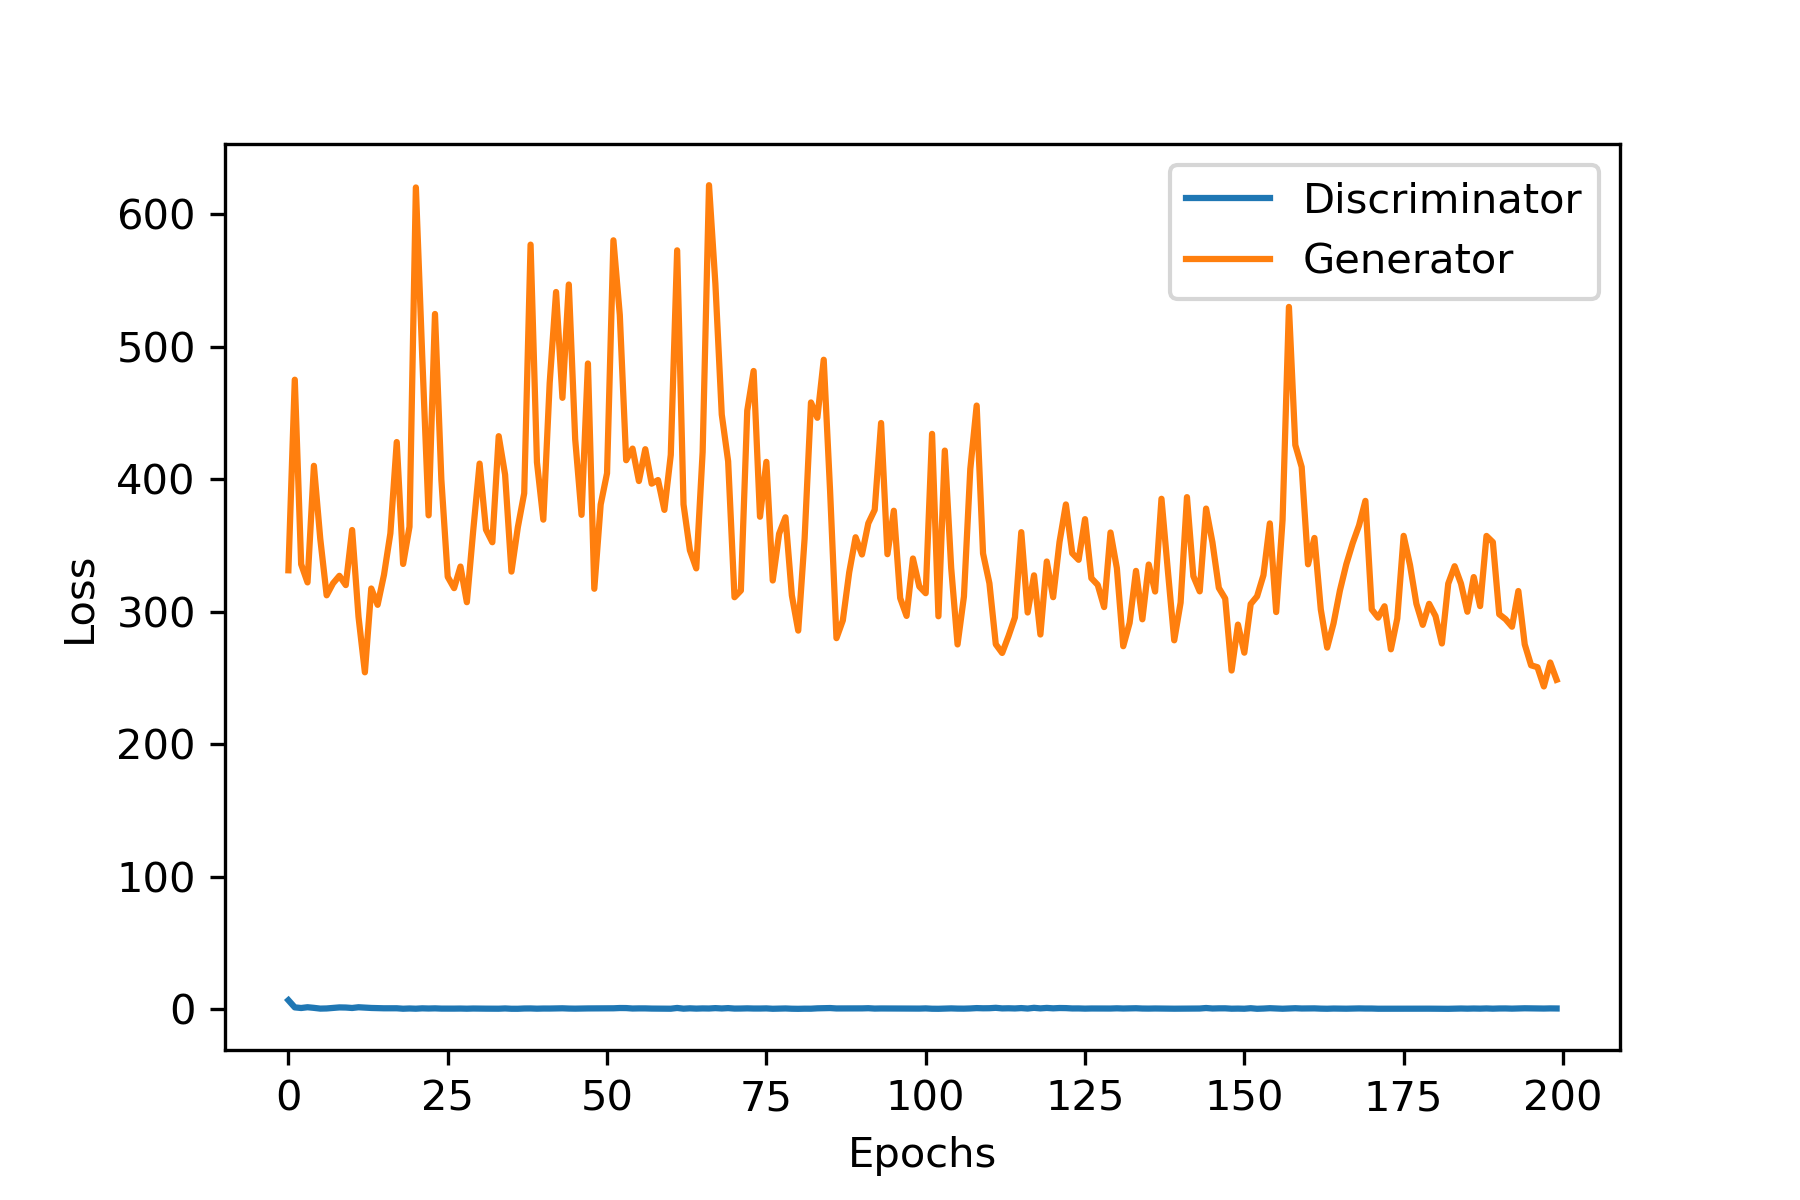
\includegraphics[width=0.48\textwidth]{0725_flute_dcgan_loss.png}
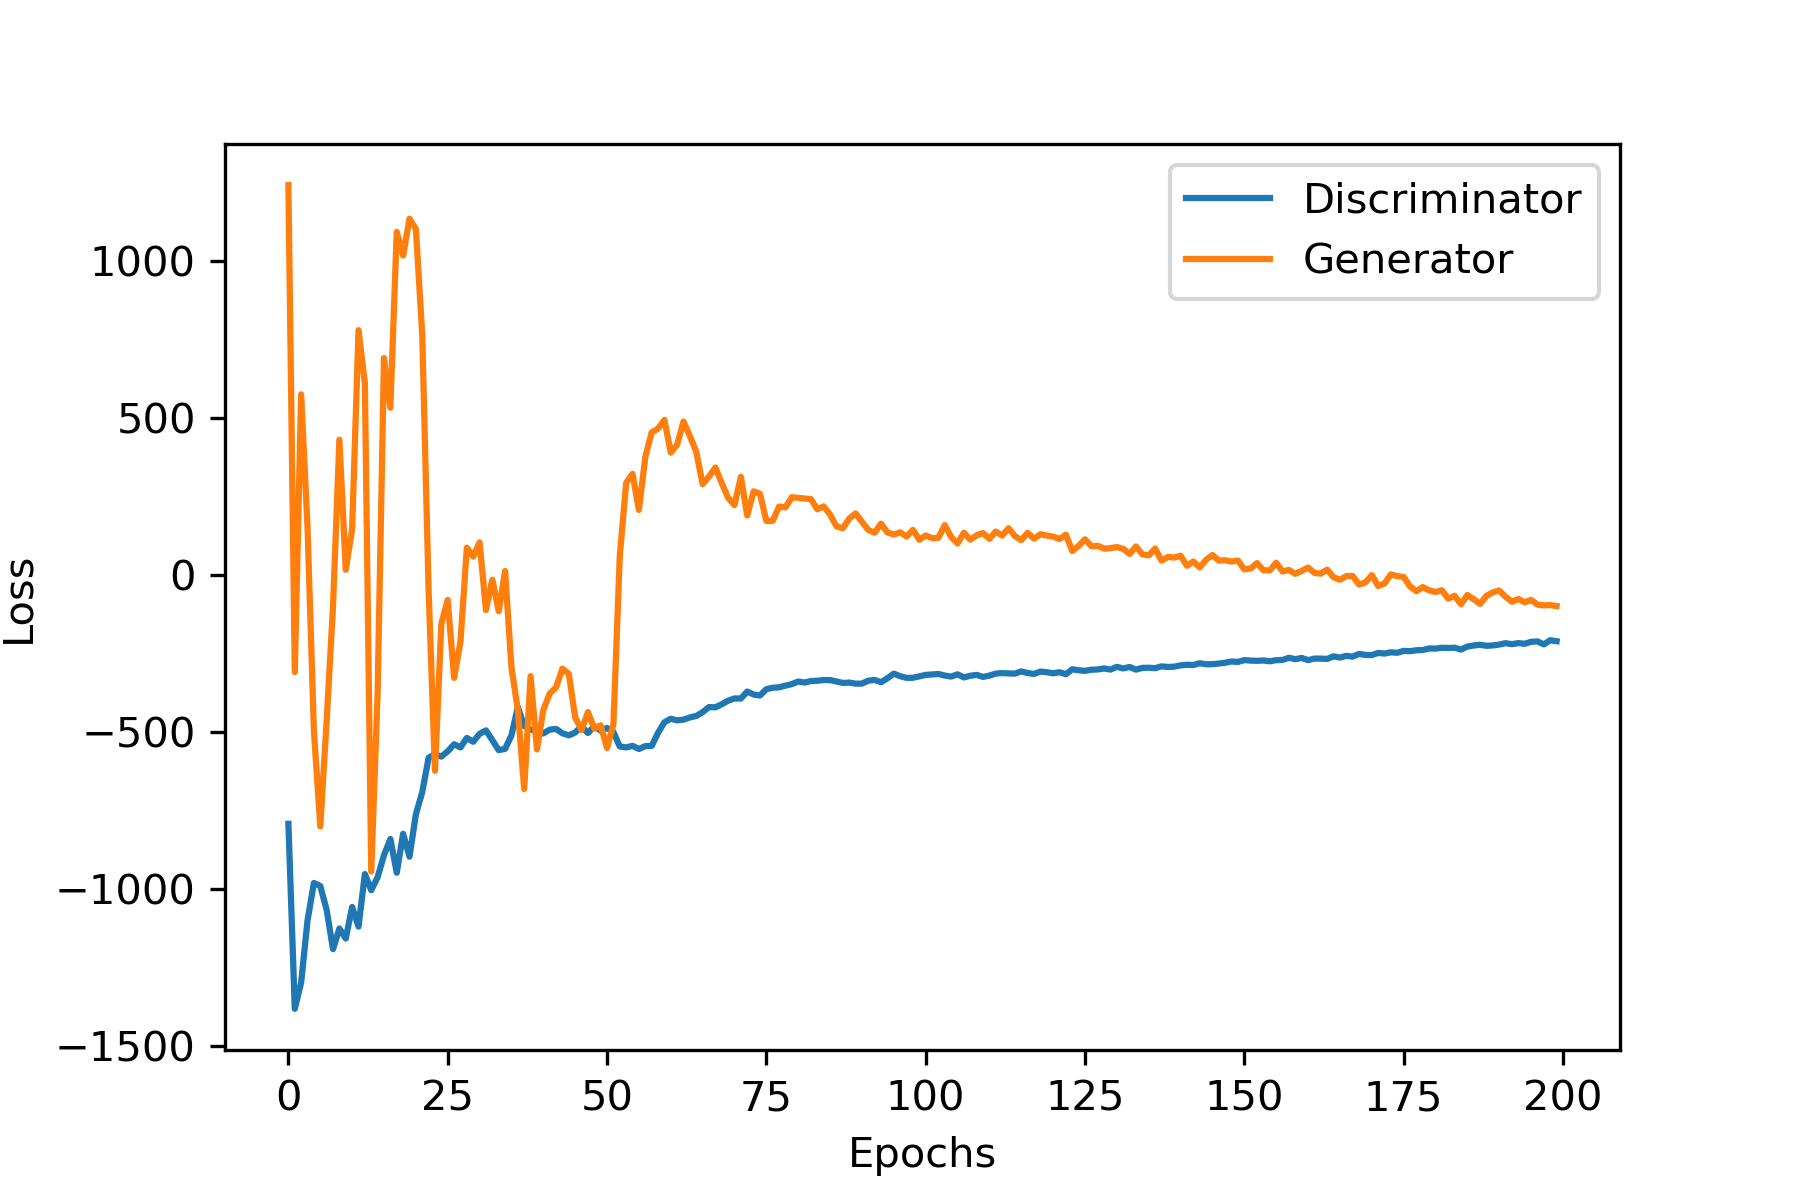
\includegraphics[width=0.48\textwidth]{0725_flute_wpgan_loss.png}
\caption{Left: typical discriminator/generator loss graphs for the naive (strong-topology) GAN. Right: typical discriminator/generator loss graphs for the WGAN-GP.}
\end{figure}\label{dcgan_wpgan}

\subsection{Single Pitch Flute Experiments}
\label{sec:single_pitch_experiments}
In this set of experiments, the GAN architecture was modified using the methods outlined in section \ref{sec:variation} through iterative experiments. During an informal evaluation of the results produced using all flute samples, we noted that it sounded like the generator was trying to produce musical scales or play multiple pitch values at once. Because this dataset contained a wide range different pitches, we hypothesized that this was forcing the generator to learn to pitch of the sound in addition to the timbre of the flute. A decision was made to remove the dimension of pitch and only train using a subset of flute sounds that contained the same pitch. The pitch that contained the most examples was selected. This resulted in a dataset of 177 flute examples playing an F. Each experiment was trained over 1000 epoch using a reduced batch size of 32 to allow the model to be trained on a GPU.

The first set of experiments was focused on the upsampling method in the generator. Five different methods were tested: transpose convolution, upsampling layer, nearest neighbor interpolation, linear interpolation, and cubic interpolation. Out of these methods linear interpolation and cubic interpolation produced poor results judged by an informal listening evaluation and were discarded for subsequent experiments. Batch normalization was then tested using transpose convolution, upsampling, and nearest neighbour interpolation. Experiments with dropout of 50\% were conducted and showed an impressive improvement in reducing noise. Phase shuffling with $N=2$ and kernel sizes $k \in \{5,15,25\}$ were finally tested. Plots of the result discriminator and generator loss for all experiments are provided in Appendix C.

\subsection{Instrument Experiments}
Based on the findings from the single pitch flute experiments, which were evaluated using a combination of nearest neighbour evaluation (described in section \ref{sec:nearest_evaluation}) and an informal subjective evaluation, a model architecture was selected for further training. The selected model used nearest neighbour interpolation, batch normalization, and a drop out of 50\% in the generator, and a kernel size of 25 in the discriminator. Using this, five new generators were trained on flute, guitar, mallet, synth bass, and vocal samples from the NSynth dataset. Single pitches were again selected for each of the datasets, and the pitch that contained a relatively large number of samples within each dataset was selected to maximize the number of samples for each set. Table \ref{tab:single_inst} provides an overview of each of these datasets.

\begin{table}[t]
    \caption{Single Pitch Instrument Training Datasets}
    \label{tab:single_inst}
    \centering
    \begin{tabular}{llll}
        \toprule
        Instrument& MIDI Note& Pitch& Num Samples\\
        \midrule
        Flute&      77&     F5&     177\\
        Guitar&     68&     G\#4&   372\\
        Mallet&     67&     G4&     355\\
        Synth Bass& 39&     D\#2&   660\\
        Vocal&      61&     C\#4&   190\\
        \bottomrule
    \end{tabular}

\end{table}



Each of the flute and mallet GANs were trained for 4000 epochs using a batch size of 32, and then due to limitations on training time, the remaining models were trained for 2000 epochs using a batch size of 32.

\subsection{MelGAN}
A number of experiments were performed using the MelGAN model described in section \ref{sec:methods_melgan}. The single pitch flute dataset that was used in the previous experiments was converted to mel-spectrograms. Two model architectures informed from the time-domain experiments conducted in section \ref{sec:single_pitch_experiments} were selected for experimentation here: transposed convolution layers vs. nearest neighbour interpolation layers, both tested with a dropout of 50\%. Figure \ref{fig:melgan} shows a spectrogram from the training dataset and two spectrograms produced by MelGAN with nearest neighbour interpolation. These results show that the structure of the harmonics was learned quite well in the first example, although misses some of a nuance of the sound. Although checkerboard artifacts aren't visible, listening to the results reveal a noticeable and unpleasant amplitude modulation, most likely due to subtle periodic artifacts from the convolution. The timbre of the sound was represented surprisingly well, but unfortunately due to the severity of the amplitude modulation artifacts the results would not be usable. The second example, on the right, shows a large 'blob' of noise that was produced unexpectedly, again rendering this model unusable.

\begin{figure}
\centering
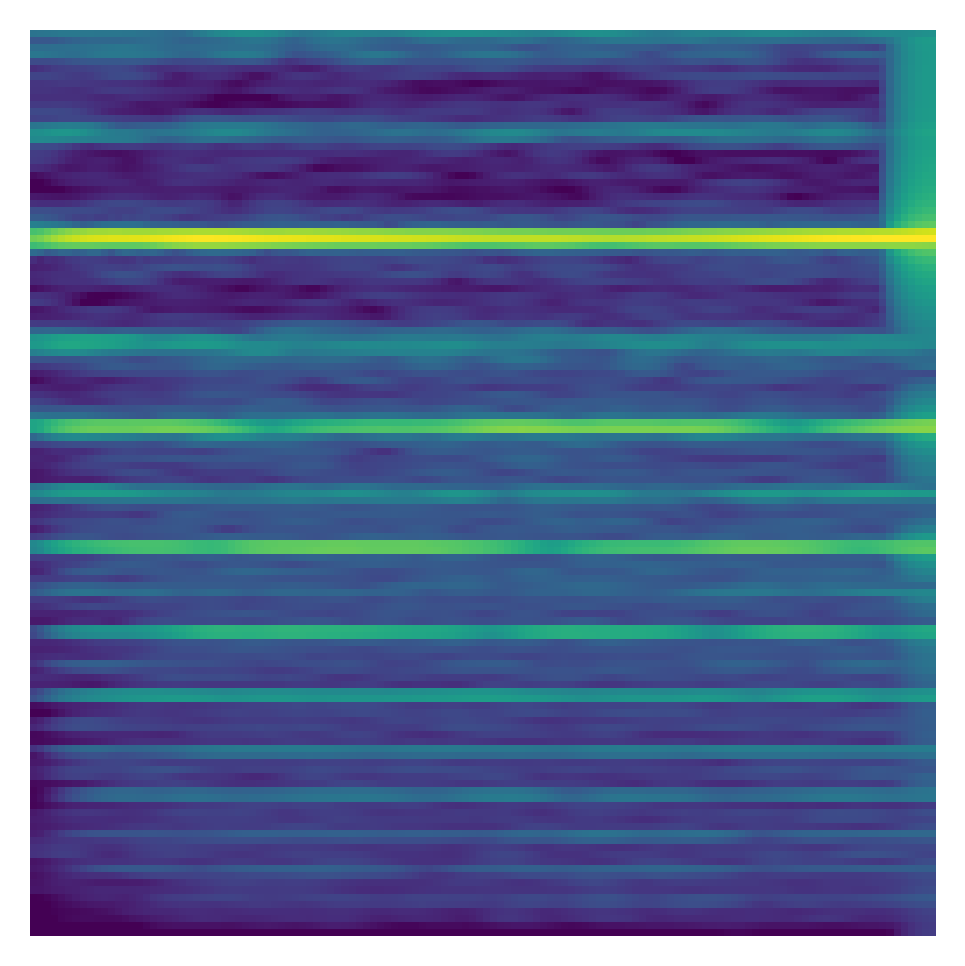
\includegraphics[width=0.32\textwidth]{MelGAN_Train.png}
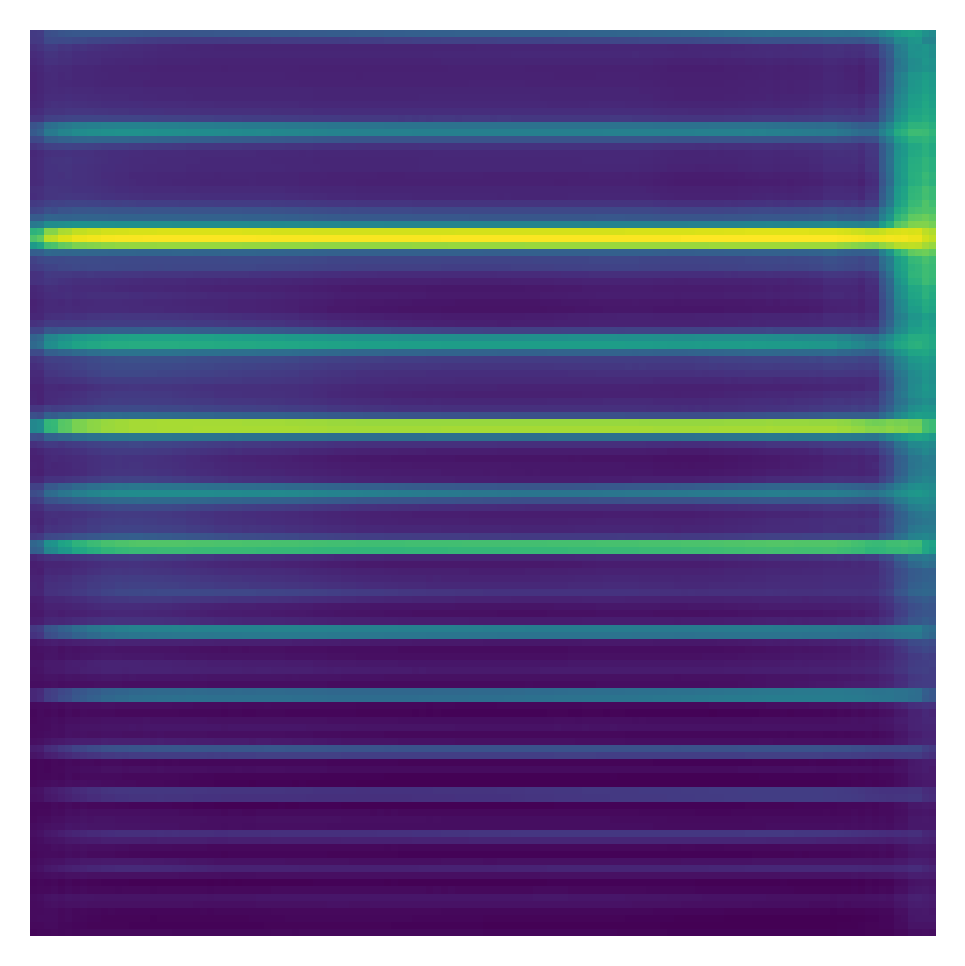
\includegraphics[width=0.32\textwidth]{MelGAN_Generated.png}
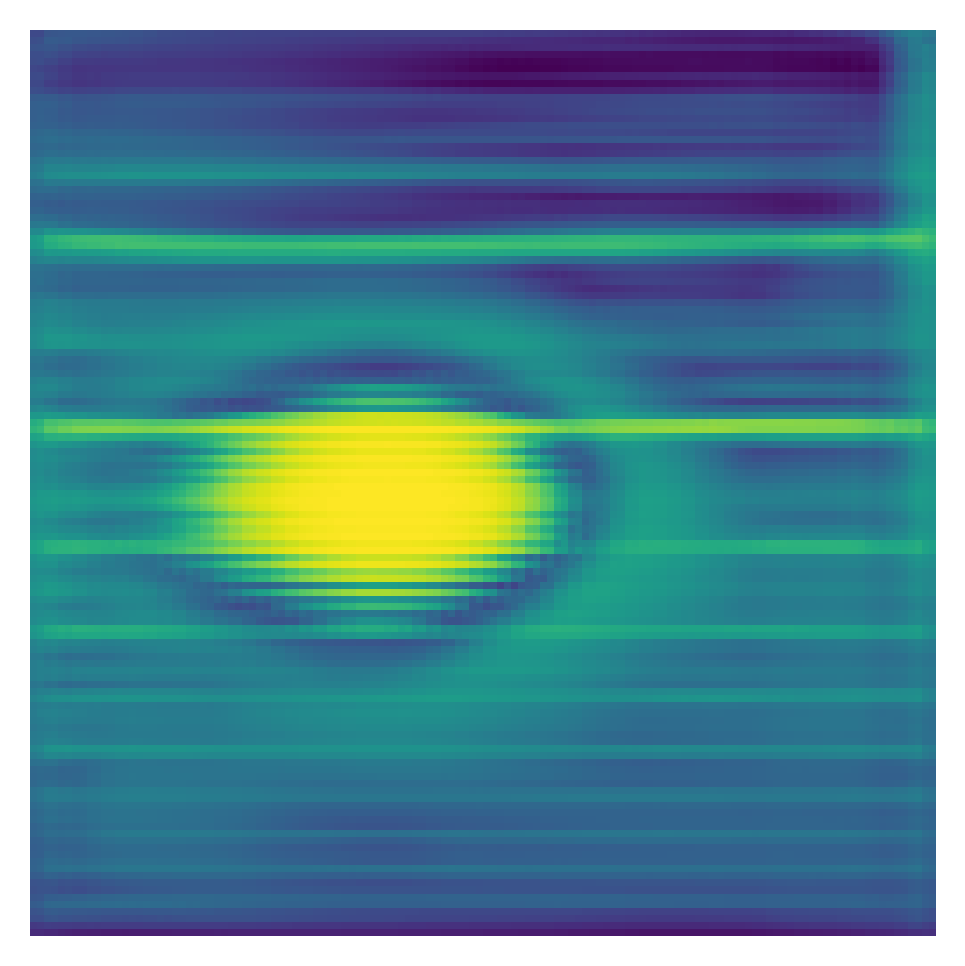
\includegraphics[width=0.32\textwidth]{MelGAN_Blob.png}
\caption{Left: Mel-Spectrogram of flute from the training set. Center and Right: Mel-Spectrograms generated by MelGAN using nearest neighbour interpolation.}
\label{fig:melgan}
\end{figure}

\subsection{Nearest Neighbour Evaluation}\label{sec:nearest_evaluation}
Nearest neighbour is an objective evaluation method proposed by \cite{donahue2018adversarial} and comprises two metrics: $|D|_{self}$ and $|D|_{train}$. $|D|_{self}$ is calculated on a set of samples and is calculated by taking the average Euclidian distance between each sample and its nearest neighbour (excluding itself). This metric provides a measurement of how much variance there is within a dataset. Smaller values of $|D|_{self}$ indicates less variance, and a value of 0 for a generator means that the generator is just producing the same result regardless of the latent input. $|D|_{train}$ is calculated by measuring the average Euclidian distance between every sample in a set of generated samples and its nearest neighbour in the dataset used for training. $|D|_{train}$ provides a measurement of how similar a set of generated samples is to the training dataset, and both measurements together provide insight into how close a generator is getting to the training dataset and the amount of variety the generator is able to learn.

Because time domain audio signals do not provide a measurement that is representative of human perception, 20 Mel-Frequency Cepstral Coefficients (MFCCs) are extracted from each signal and summarized over time using the mean.

\subsubsection{Single Pitch Flute Evaluation}
Evaluation of the models generated from experiments conducted using the single pitch flute dataset (Section \ref{sec:single_pitch_experiments}) was performed by generating 200 random audio samples from each trained model. This resulted in 14 different generated datasets that were evaluated using the two nearest neighbour metrics. The flute training dataset was included in the $|D|_{self}$ measurement. These results are shown in figure \ref{fig:single_pitch_nn}. 

The $|D|_{self}$ results confirm that both linear and cubic interpolation produced results that were not close to the training dataset, and that nearest neighbour interpolation performed the best out of all the resize methods. Adding dropout to the generator had a significant effect on improving the generator's ability to learn the distribution of the flute dataset. Interestingly, increasing the kernel size did not have a hugely significant effect on the learning once dropout had been added. Another interesting result is that several of the models actually produced results that had both greater variance than the training dataset while also having a small value 

\begin{figure}[htbp]
\centering
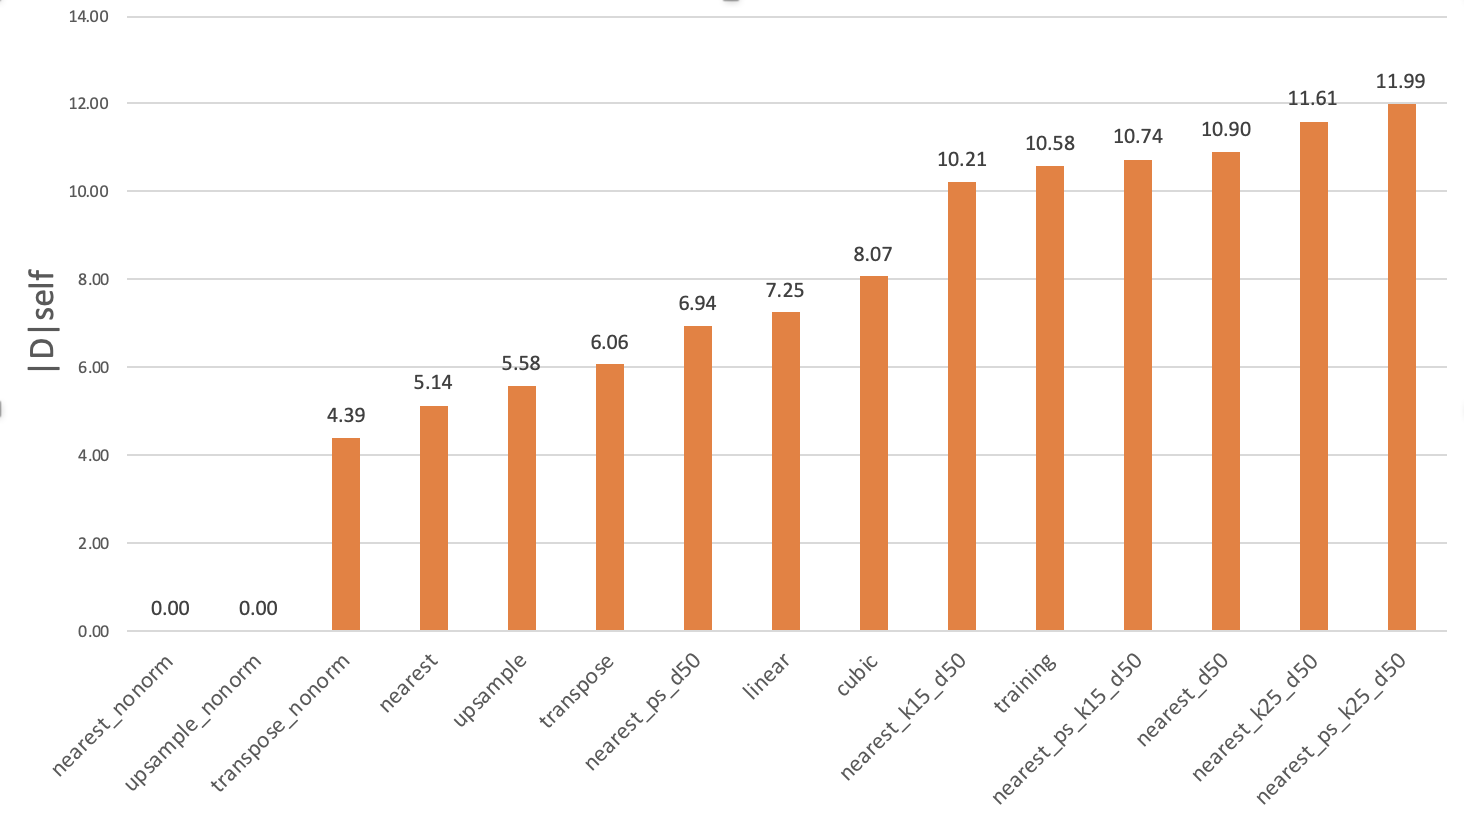
\includegraphics[width=0.75\textwidth]{D_self.png}
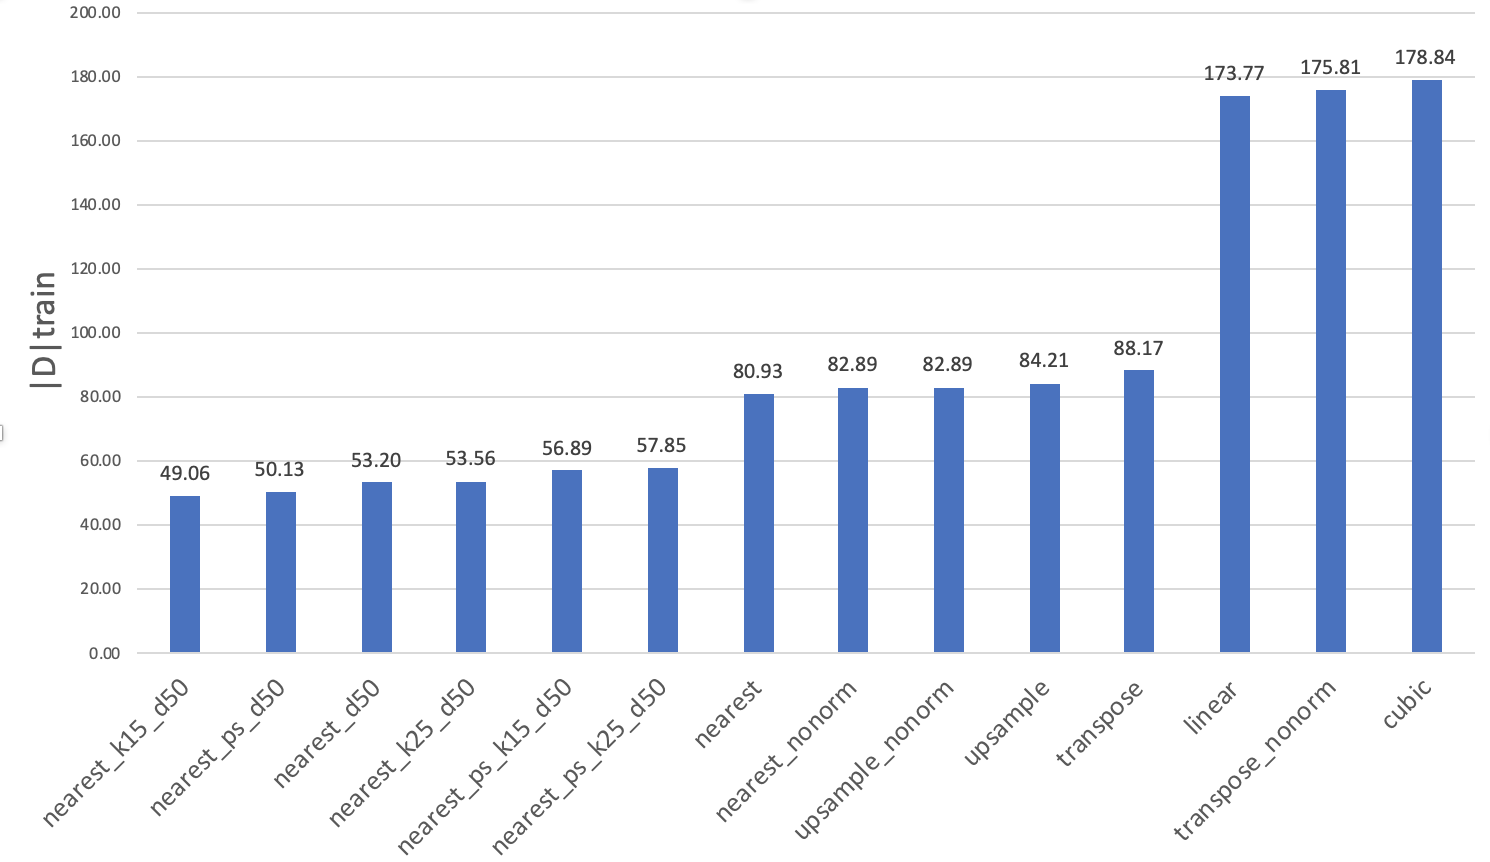
\includegraphics[width=0.75\textwidth]{D_train.png}
\caption{Nearest neighbour evaluation for the single pitch flute experiments. Top: $|D|_{self}$ . Bottom $|D|_{train}$. The model type is indicated in the x-axis by a string giving the upsampling method and then appending any additional changes, where nonorm indicates no batch normalization in the generator, ps indicates phase shuffling in the discriminator, k$n$ indicates the kernel size in the discriminator where $n$ is the kernel size, if no k is provided then the kernel size is 5, and d50 indicates that dropout of 50\% was used in the generator.}
\label{fig:single_pitch_nn}
\end{figure}

\subsubsection{Single Pitch Instrument Evaluation}
Evaluation of the models generated from training the different instrument datasets was performed by generating 500 random audio samples from each trained model: flute, guitar, mallet, synth bass, and vocal. Each of these generated datasets were evaluated using the two nearest neighbour metrics. The datasets used to train each of the models is included in the $|D|_{self}$ metrics. These results are shown in figure \ref{fig:instrument_nn}. Results of $|D|_{train}$ show that the other instrument datasets had more variance between samples than those of the flute dataset, and that the models trained from the datasets did not have the same degree of variance between samples. The results of $|D|_{self}$ are comparable for all training datasets, the mallet generator was closest to the training dataset and the synth bass was most dissimilar.

\begin{figure}[htpb]
\centering
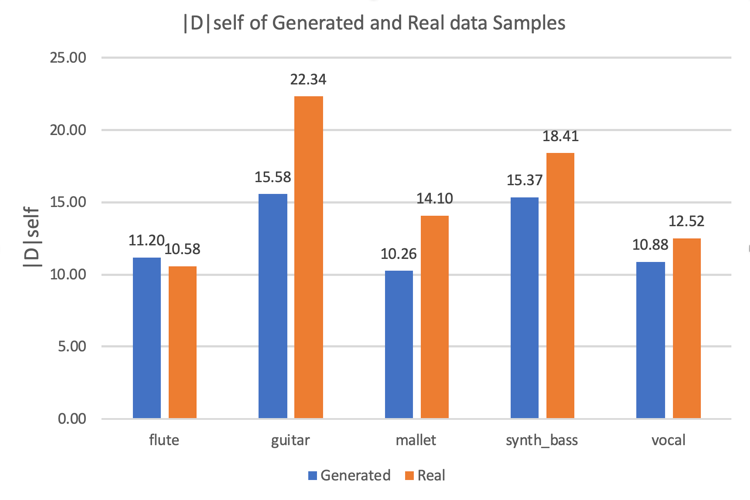
\includegraphics[width=0.49\textwidth]{D_self_gen_real_2.png}
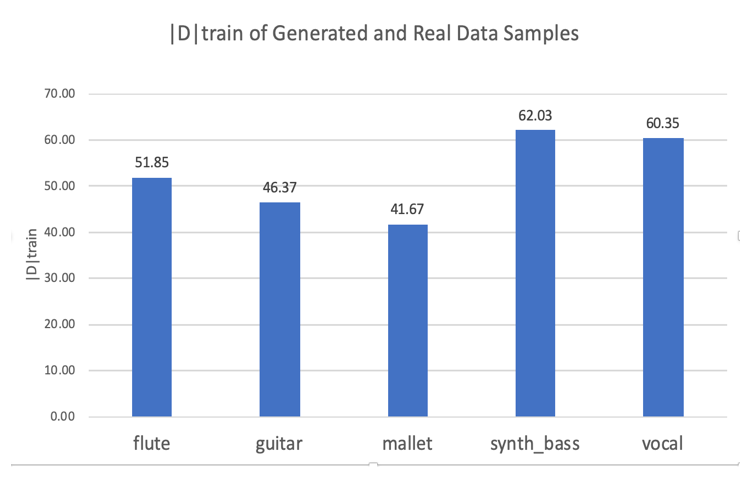
\includegraphics[width=0.49\textwidth]{D_train_gen_real_2.png}
\caption{Nearest neighbour evaluation for the instrument experiments. Top: $|D|_{self}$ . Bottom $|D|_{train}$.}
\label{fig:instrument_nn}
\end{figure}

%\subsection{Qualitative Results}
%Show some plots of the waveform learning, perhaps show some error cases (like the weird hole in the Mel-Spectrogram). PCA plot of the flute learning.

\section{Discussion and Conclusion}

Audio generation in GANs is a relatively unexplored field, especially considered to the sister field of image generation. Our results have been promising, but far from complete. The generated samples have been far from passing any sort of subjective-evaluation Turing tests; however, our generated samples do capture certain key components of the instrument. Both veins of GAN we tried (time-series based and mel-frequency based) exhibited positive and negative features which were in some sense complementary from the other.

The time-series based WaveGAN-like networks were able to generate sounds which were structurally similar to the originals, except that they failed to capture high frequency components of the signal. This could be an effect of the reduced sample rate, or due to the resizing methods we explored. While transpose convolutions are more likely to produce aliasing and noise related to checkerboard artifacts, \cite{donahue2018adversarial} note that these transpose convolution layers may be important in generating high-frequency detail.

The mel-spectrogram-based approach, on the other hand, captured the timbre of the sound fairly well. However, it suffered from the opposite problem as the time-series based networks: structurally, the samples were off, carrying unnatural ``fluttering'' artifacts. These artifacts could be related to ``bump'' artifacts we noticed in the center of some training samples' spectrograms. It is a little puzzling that the discriminator was not able to catch and prevent these artifacts. However, it is rather encouraging that this may be is the stumbling block on which the MelGAN failed. For, preventing these artifacts is a clearly-defined problem in the realm of image generation. It is therefore possible to bring the full brunt of image-based GAN technology to bear on the problem. Furthermore, checkerboard artifacts may be involved, creating strange discontinuities in the spectrum and overemphasizing certain spectral bands.

The resize/upsampling-based approaches were moderately successful in eliminating these checkerboard artifacts. Only nearest-neighbor-style resizing as able to train well;  the generators equipped with either cubic or linear interpolation struggled to improve over time. This agrees with observations made in \cite{Odena2016DeconvolutionAC}: the current state-of-the-art hyperparameters are tuned to efficiently train transpose convolution based generators, which are analogous to nearest-neighbor upsampling based generators. Odena et al. hypothesized that better results may be obtained after a careful search of hyperparameter space aimed at improving cubic interpolation based generators. This is an exciting research avenue which may well yield tremendous improvements in sound quality.

By far, the greatest improvement in sound quality came as a result of adding dropout layers to the neural network. Previously, the networks had only been generating very grating ``rusty doorhinge'' sounds. Dropout layers significantly regularized the samples and made them palatable to the human ear. Because dropout layers are resistant to overtraining, it is possible that training the networks for even longer while using dropout layers would yield improved results.

Because we were only considering the first second of the 4-second-long NSynth samples, it was not possible in general for the GAN to interact with the entire envelope of the samples (except for samples with fast decay, such as the mallet sounds). Our results were therefore generally limited to capturing the samples' attack and timbre. These two properties, however, largely dominate the quality and recognizably of a sound.

One philosophical observation is that in an ideal world, machine learning specialists are able to bring their human intuitions about the structure of a problem to bear on the network architecture. This partially explains the tremendous success of convolutional neural networks in image-related problems: convolution captures salient properties of images, namely spacial proximity and approximate translation-invariance of features (for example the first layer of a CNN tends to capture different types of lines in an image, which are clearly invariant of position on the image).

It is interesting to ponder whether or not the DCGAN architecture captures the relevant features in sound generation. The approach in \cite{donahue2018adversarial}, and in our own work, was to transport successes in image generation with minimal alteration into the field of audio generation. It may be that this is a case of square pegs and round holes.

For example, it is not obvious a priori that convolution in one dimension even `sees' timbre: after all, adjacency in `physical space' is very different from adjacency in spectral space, while spectral space is arguably what we are really noticing when we listen to audio.

The MelGAN has direct access to the spectrum of a sound, and therefore locality on the spectrogram is a reasonable thing to assume. However, the translational invariance property of CNNs is a reasonable thing to question in this context. For, while translation in the x-axis corresponds to translation in time, which is a very reasonable thing to assume translation invariance for, vertical translation is a different beast. For, the scaling of frequency bands (whether linear, logarithmic, or other) now becomes a crucial point. What is to say that ``a straight line'' in the upper frequencies of a spectrogram in any way corresponds to a straight line in the lower frequencies, especially if the straight line is not horizontal? It may be profitable to treat a spectrogram less as an image and more as a time-series of spectral coefficient vectors, perhaps by prioritizing the y axis in the network architectures.

This paper has only brushed the tip of the problem of audio generation, but even this short exploration has illuminated a vast spectrum of audio-related challenges and promising avenues for possible research.
	\graphicspath{{./}{./figures/}{./figures/torchsynth/}}

\chapter{GPU Enabled Synthesis}

In the preceding chapter I explored and compared various methods for inverse synthesis, which is one approach to automatic synthesizer programming. These experiments highlighted some of the challenges that researchers are faced with in this work. The most daunting challenge is related to the shear complexity of the relationship between the parameter space and perceptual (auditory) space, and how much variability there is within that relationship depending on the specifics of the synthesis engine and the number and type of parameters. In addition to that, there is no accepted best approach to computationally representing the perceptual space and defining metrics within that space. It is an open question on how to answer the question "How similar are these two sounds?" in a quantifiable way with regards to timbre. The ability to perform experiments that seek to solve these challenges is hindered by additional computational challenges associated with software synthesizers. Recent research has sought to automatically program commercially available VST synthesizers. This approach is well-founded considering these synthesizers represent tools that are currently being used by music producers and sound designers. However, these synthesizes are optimized for real-time use as opposed to use in the machine learning research, where they introduce bottlenecks \cite{masudo2021quality} and difficulties with learning in gradient descent methods.

In this chapter I present a GPU-enabled modular synthesizer that was designed in response to the identified computational challenges and can be used to support research in automatic synthesizer programming. The work presented here was conducted with Joseph Turian, Max Henry, and my supervisors George Tzanetakis and Kirk McNally, and was published in the proceedings of s 


In response to these computational challenges, and out of a desire to support research that seeks to elucidate the complex relationship between synthesizer parameters and the auditory result, a GPU enabled 

\section{Introduction}
\label{sec:intro}

Machine learning progress has been driven by training regimes that leverage large corpora. The past decade has seen great progress in NLP and vision tasks using large-scale training. As early as 2007, Google \cite{brants-etal-2007-large} achieved state-of-the-art machine translation results using simple trillion-token $n$-gram language models.
Recent work like GPT3 \cite{NEURIPS2020_1457c0d6} suggests that it is preferable to do less than one epoch of training on a large corpus, rather than multiple epochs over the same examples. Even tasks with little training data can be attacked using self-supervised training on a larger, related corpus followed by a transfer-learning task-specific fine-tuning step.

\begin{table}[thb]
\begin{center}
\begin{tabular}{r|c|r|c|c}
Name & Type & \#hours & Free & Multi-modal \\
\hline
Diva \cite{esling2020flow} & synth & 12 & yes & parameters \\
FSDK50 \cite{fonseca2020fsd50k} & broad & 108 & yes & tags \\
NSynth \cite{engel2017neural} & notes & 333 & yes & tags \\
LibriSpeech \cite{librispeech} & speech & 1000 & yes & text \\ 
DAMP-VPB \cite{smule_inc_2017_2616690} & songs & 1796 & no & lyrics \\
Audioset \cite{45857} & broad & 4971 & no & video+tags \\ 
YFCC100M \cite{thomee2016yfcc100m} & broad & 8081 & yes & video \\
MSD \cite{bertin2011million} & songs & 72222 & no & tags+metadata \\
Jukebox \cite{dhariwal2020jukebox} & songs & 86667 & no & {\footnotesize lyrics+metadata}\\
synth1B1 & synth & 1111111 & yes & parameters \\
% etc let's add a few more standard corpora here
% also the SMULE zenodo singing corpus
\end{tabular}
\end{center}
\caption{Large-scale and/or synthesizer audio corpora.}
\label{tbl:audio-corpora}
\end{table}

Unfortunately, audio ML progress has been hindered by a dearth of large-scale corpora. Audio ML involves multiple epoch training on comparably small corpora compared to vision or NLP. Table~\ref{tbl:audio-corpora} summarizes various large-scale and/or synthesizer audio corpora.
For example, using AudioSet \cite{45857} requires scraping 5000 hours of Youtube videos, many of which become unavailable over time (thus impeding experimental control). FSD50K \cite{fonseca2020fsd50k}, a free corpus, was recently released to mitigate these issues, but contains only 108 hours of audio. To the best knowledge of the authors, the largest audio set used in published research is Jukebox \cite{dhariwal2020jukebox}, which scraped 1.2M songs and their corresponding lyrics. Assuming average song length is 4:20, we estimate their corpus is $\approx$90K hours. 



\subsection{Background and Motivation}

\subsubsection{Pre-training and learned representations}

Tobin {\em et al.}~\cite{DBLP:conf/iros/TobinFRSZA17} argue that learning over synthesized data enables transfer learning to the real-world.
Multi-modal training offers additional benefits.
Images evince sizes of objects immediately, while object size is difficult to glean through pure linguistic analysis of large corpora  \cite{DBLP:conf/acl/ElazarMRBR19}.
Multi-model learning of audio---with video in \cite{DBLP:conf/icassp/CramerWSB19} and semantic tags in \cite{drossos:icml:2020}---has led to strong audio representations.
Constrastive audio learning approaches like \cite{saeed2020contrastive} can be used in multi-modal settings, for example by learning the correspondence between a synthesized sound and its underlying parameters.
% Later, cite BYOL-A if their paper is selected
However, training such models is limited by small corpora and/or the relatively slow synthesis speed of traditional CPU-based synths (Niizumi, p.c.).

% Going to pull out some of this to the 
% \subsubsection{Software Synthesizers}

% Programming audio synthesizers is challenging and requires a technical understanding of sound design to fully realize their expressive power. Traditional synthesizers can have over 100 parameters that affect audio generation in complex, non-linear ways. One of the most commercially successful audio synthesizers, the Yamaha DX7, was notoriously challenging to program. Allegedly nine out of ten DX7s coming into workshops for servicing still had their factory presets intact \cite{seago2004critical}.

% Since the early 90s, researchers have leveraged advances in ML to develop a deeper understanding of the synthesizer parameter space and to build more intuitive methods for interaction \cite{horner1993machine}. Recently, deep learning has been used for programming synthesizers.  Esling {\em et al.}\ \cite{esling2020flow} trained an auto-encoder network to program the \href{https://u-he.com/products/diva/}{U-He Diva} using 11K synthesized sounds with known preset values. Yee-King {\em et al.} \cite{yee2018automatic} used a recurrent network to automatically find parameters for \href{https://asb2m10.github.io/dexed/}{Dexed}, an open-source software emulation of the DX7.

% \subsubsection{Neural Synthesis}

% In contrast to traditional synthesis, neural synthesizers generate audio using large-scale machine learning architectures with millions of parameters \cite{engel2017neural}. Differentiable digital signal processing \cite{engel2020ddsp} bridged the gap between traditional DSP synthesizers with the expressiveness of neural networks, exploring a harmonic model-based approach, using a more compact architecture with 100K parameters.
% One benefit of synthesized audio is that the underlying factors of variation ({\em i.e.}~the parameters) are known. We combine the ideas of traditional DSP and neural synthesis, yielding a greater level of simplicity and speed by building a GPU-optional modular synthesizer. Our default voice has 78 latent parameters, which model traditional synthesizer parameters. 

\section{Main Contributions}
\label{sec:contributions}

Our synth1B1 corpus and torchsynth software provide a fast, open approach for researchers to do large-scale audio ML pre-training and develop a deeper understanding of the complex relationship between the synthesizer parameter space and resulting audio.
A variety of existing research problems can use synth1B1, including:
\begin{itemize}
\item Perceptual research into audio, such as crafting auditory distance measures and inferring timbre dimensions. \cite{vahidi2020timbre}
\item Inverse synthesis, i.e.\ mapping from audio to underlying synthesis parameters.
\cite{yee2018automatic,esling2020flow}
\item Inferring macro-parameters of synthesizers that are more perceptually relevant. \cite{esling2020flow, tatar2021latent}
%\item Transfer learning for automatic programming of black-box software synthesizers.
\item Audio-to-MIDI. \cite{47659}
\item Imitation of natural sounds with established synthesis architectures.
\end{itemize}
%% can you think of more?
Researchers can also use the synth1B1 corpus to arbitrage innovations from adjacent ML fields, namely: large-scale multi-modal, self-supervised, and/or contrastive learning, and transfer-learning through fine-tuning on the downstream task of interest, particularly tasks with few labeled examples.

\subsection{synth1B1}

synth1B1 is a corpus consisting of one million hours of audio: one billion 4-second synthesized sounds. The corpus is multi-modal: Each sound includes its corresponding synthesis parameters. We use deterministic random number generation to ensure replicability, even of noise oscillators. One tenth of the examples are designated as the test set. Researchers can denote subsamples of this corpus as synth1M1, synth10M1, {\em etc.} % which would refer to the first 1 million and 10 million samples of Synth1B1 respectively.

Data augmentation has been used on small-scale corpora to increase the amount of labeled training data. As discussed in \S\ref{sec:intro}, large-scale one-epoch training is preferable, which is possible using synth1B1's million-audio-hours.

Besides sheer size, another benefit of synth1B1 is that it is multi-modal: instances consist of both audio {\em and} the underlying parameters used to generate this audio. The use of traditional synthesis paradigms allows researchers to explore the complex interaction between synthesizer parameter settings and the resulting audio in a thorough and comprehensive way. 
Large-scale contrastive learning typically requires data augmentation ({\em e.g.}\ image or spectrogram deformations) to construct positive contrastive-pairs \cite{pmlr-v119-chen20j,DBLP:journals/corr/abs-2103-06695}. However, this sort of faux-constrastive-pair creation is not necessary when the underlying latent parameters are known in a corresponding modality.

\subsection{torchsynth}

synth1B1 is generated {\em on the fly} by \href{https://github.com/torchsynth/torchsynth}{torchsynth 1.0}.
% TODO: pypi package
% TODO: We could make a 'torchsynth' github org rather than using my namespace
torchsynth is an open-source modular synthesizer and is GPU-enabled. torchsynth renders audio at 16200x real-time on a single V100 GPU. Audio rendered on the GPU can be used in downstream GPU learning tasks without the need for expensive CPU-to-GPU move operations, not to mention disk reads. It is faster to render synth1B1 {\em in-situ} than to download it. torchsynth includes a replicable script for generating synth1B1.
 %Many modules in torchsynth 1.0 are differentiable but backprop has not been stress-tested in this release, as our focus has been fast inference and perceptual sonic diversity. % [also the discussion on those guys that did their own differentiation things from FB chat]
To accommodate researchers with smaller GPUs, the default batchsize is 128, which requires between 1.9 and 2.4 GB of GPU memory, depending upon the GPU.
%The nomenclature ``synth1B1-312-6'' denotes batch 312 and sound 6 within that batch.
If a train/test split is desired, 10\% of the samples are marked as test. Because researchers with larger GPUs seek higher-throughput with batchsize 1024, $9 \cdot 1024$ samples are designated as train, the next 1024 samples as test, {\em etc.} The default sampling rate is 44.1kHz. However, sounds can be rendered at any desired sample rate. %, such as 96kHz, for use in high-resolution applications.
% What about fp16?
Detailed instructions are contained at the torchsynth URL for the precise protocol for replicably generating synth1B1 and sub-samples thereof. %(See profiling in Section [...]).

% We might also need to be careful because if we exhaust the space of possible sounds of the synthesizer, then a simple KNN approach will find the right parameters.

%JND experiments demonstrates that [...]\% of audio samples are perceptually different to human listeners.
%[multimodal]

\subsection{Questions in Synthesizer Design, and New Pitch and Timbre Datasets and Benchmarks}

When generating synthesized datasets, one needs to sample the parameter space. Typically this is achieved through na\"ively sampling parameters uniformly and rendering the resulting audio. Due to the complexity of the parameter space and interaction between parameters, this may lead to a large number of redundant, extreme frequency, and/or unnatural sounds. We propose several new open challenges in synthesizer design, specifically focusing on the task of designing parameters and sampling them, including:
\begin{itemize}
    \item How do you measure the perceptual diversity of a synthesizer's sounds? How do you maximize it?
    \item How do you tune a synthesizer to imitate existing synthesizers? Is there a way to sample the parameters so the resulting audio sounds like a human-designed preset?
\end{itemize}
In \S\ref{sec:hyperparameter-tuning} we demonstrate a principled approach to attacking these tasks. The main research barrier to solving these tasks is the lack of an automatic, perceptually-relevant auditory distance measures.
To evaluate existing auditory distance measures, we devise two new evaluation methodologies and concurrently release timbre and pitch-datasets, each representing 22.5 and 3.4 hours of audio respectively, for the following open-source synthesizers: a \href{https://github.com/bwhitman/learnfm}{DX7} clone and \href{https://surge-synthesizer.github.io/}{Surge}, as \href{https://zenodo.org/record/4677102}{DOI 10/f7dg} and \href{https://zenodo.org/record/4677097}{DOI 10/f652}, respectively. These datasets represent ``natural'' synthesis sounds---i.e.\ presets designed by humans, not just a computer randomly flipping knobs---which we use in two ways: a) New benchmarks for evaluating audio representations. b) Evaluating the similarity of different sound corpora.
%[Secret Sauce data if they grant us license] Lastly, we release a standardized format for describing the parameter settings and appropriate ranges and scaling.


\section{Design Methodology}
\label{sec:design-methodology}
\subsection{Synth Modules}
torchsynth's design is inspired by hardware modular synthesizers which contain individual units. Each module has a specific function and parameters, and they can be connected together in various configurations to construct a synthesizer. There are three types of modules in torchsynth: audio modules, control modules, and parameter modules. Audio modules operate at audio sampling rate (default 44.1kHz) and output audio signals. Examples include voltage-controlled oscillators (VCOs) and voltage-controlled amplifiers (VCAs). Control modules output control signals that modulate the parameters of another module. For speed, these modules operate at a reduced control rate (default 441Hz). Examples of control modules include ADSR envelope generators and low frequency oscillators (LFOs). Parameter modules simply output parameters. An example is the monophonic ``keyboard'' module that has no input, and outputs the note midi f0 value and duration.

To take advantage of the parallel processing power of a GPU, all modules render audio in batches. Larger batches enable higher throughput on GPUs.  Figure~\ref{fig:gpu-profiles} shows torchsynth's throughput at various batch sizes on a single GPU. GPU memory consumption $\approxeq 1216 + (8.19\ \cdot $ batch\_size) MB, including the torchsynth model. The default batch size 128 requires $\approx$2.3GB of GPU memory, and is 16200x faster than realtime on a single V100 GPU. %Any multiple of 128 batch-size is supported and synth1B1 will be deterministically rendered for scientific reproducibility.
A batch of 4 of randomly generated ADSR envelopes is shown in Figure~\ref{fig:adsr}.


%\renewcommand{\thesubfigure}{Figure %\arabic{subfigure}}

\begin{figure}[t]
    \centering
    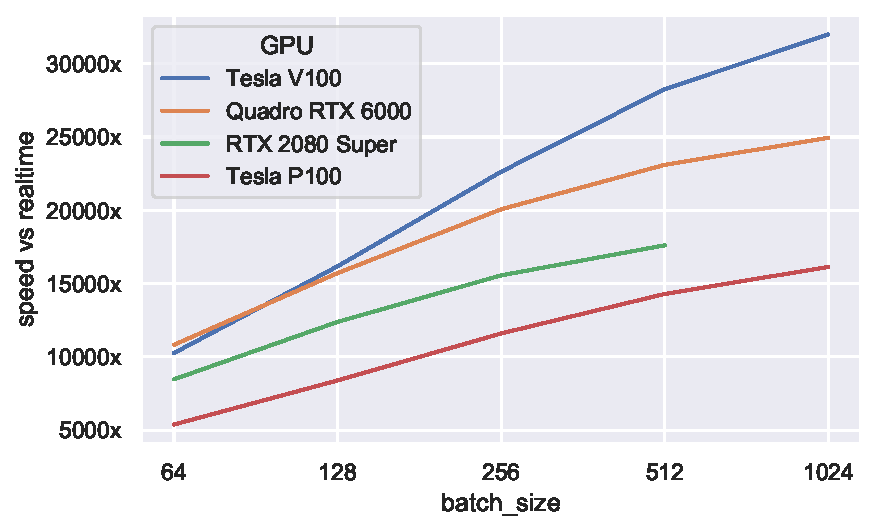
\includegraphics[width=0.66\linewidth]{gpu-profiles.pdf}
  \vspace{-1.5em}
    \caption{torchsynth throughput at various batch sizes.}
    \label{fig:gpu-profiles}
\end{figure}

\begin{figure}[t]
    \centering
    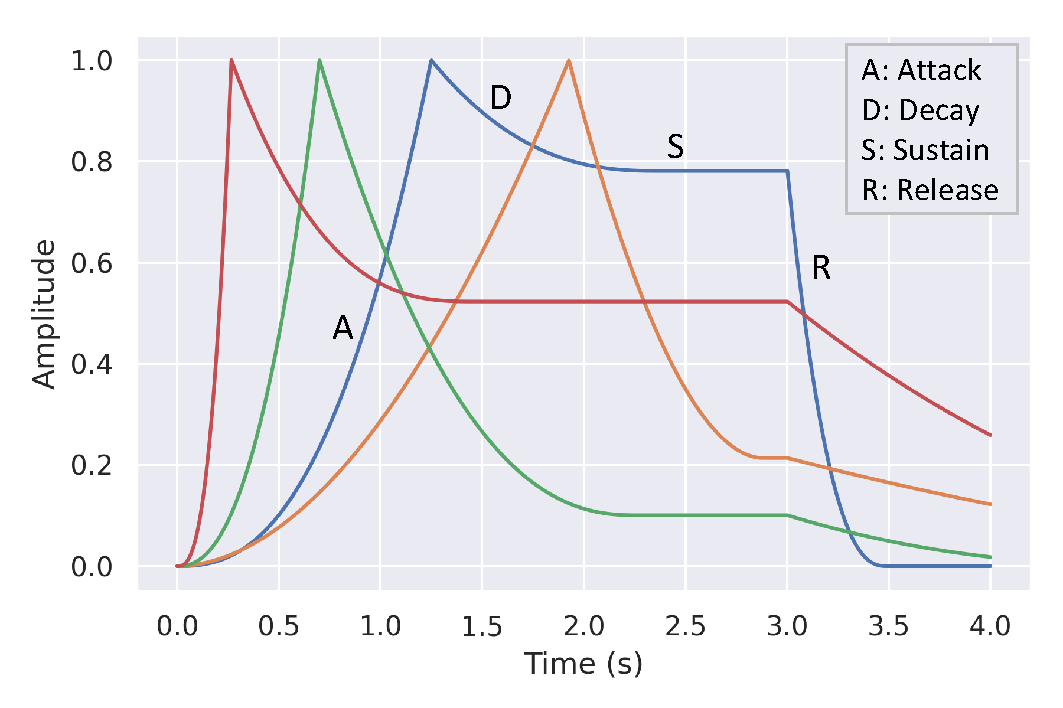
\includegraphics[width=0.66\linewidth]{ADSR.pdf}
%    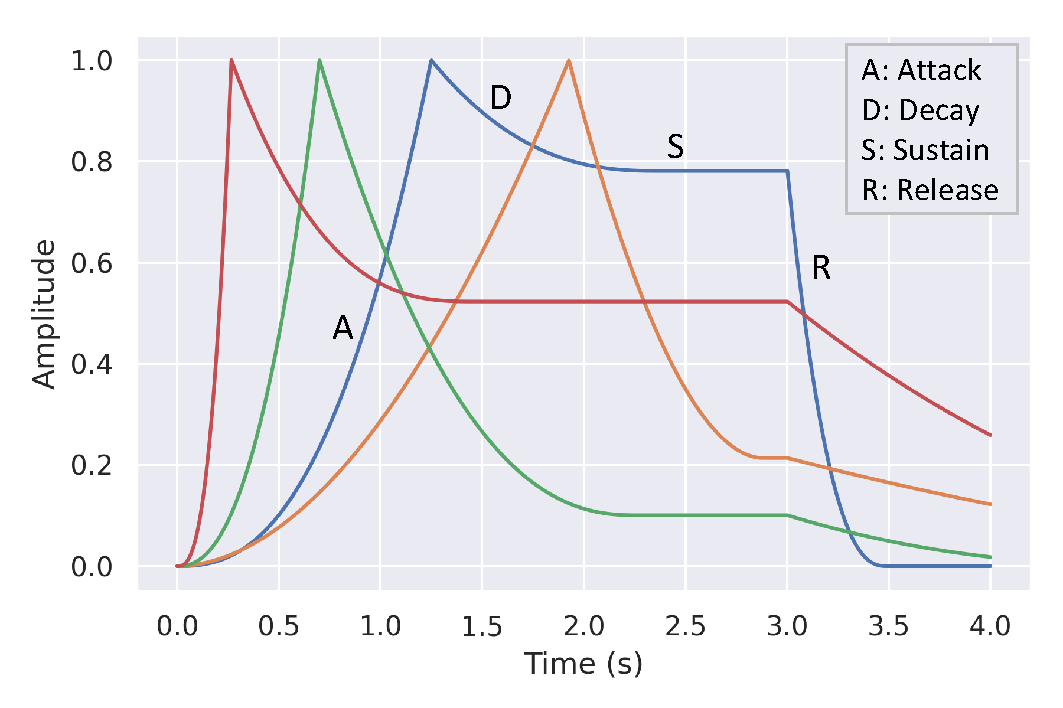
\includegraphics[width=0.95\linewidth]{ADSR.pdf}
  \vspace{-1.5em}
    \caption{Batch of four randomly generated ADSR envelopes.
    Each section for one of the envelopes is labelled.}
    \label{fig:adsr}
\end{figure}

\subsection{Synth Architectures}

The default configuration in torchsynth is the Voice, which is the architecture used in synth1B1. The Voice comprises the following modules: a Monophonic Keyboard, two LFOs, six ADSR envelopes (each LFO module includes two dedicated ADSRs: one for rate modulation and another for amplitude modulation), one Sine VCO, one SquareSaw VCO, one Noise generator, VCAs, a Modulation Mixer and an Audio Mixer. Modulation signals generated from control modules (ADSR and LFO) are upsampled to the audio sample rate before being passed to audio rate modules. Figure \ref{fig:voice_diagram} shows the configuration and routing of the modules comprised by Voice. 

\begin{figure}[t]
    \centering
    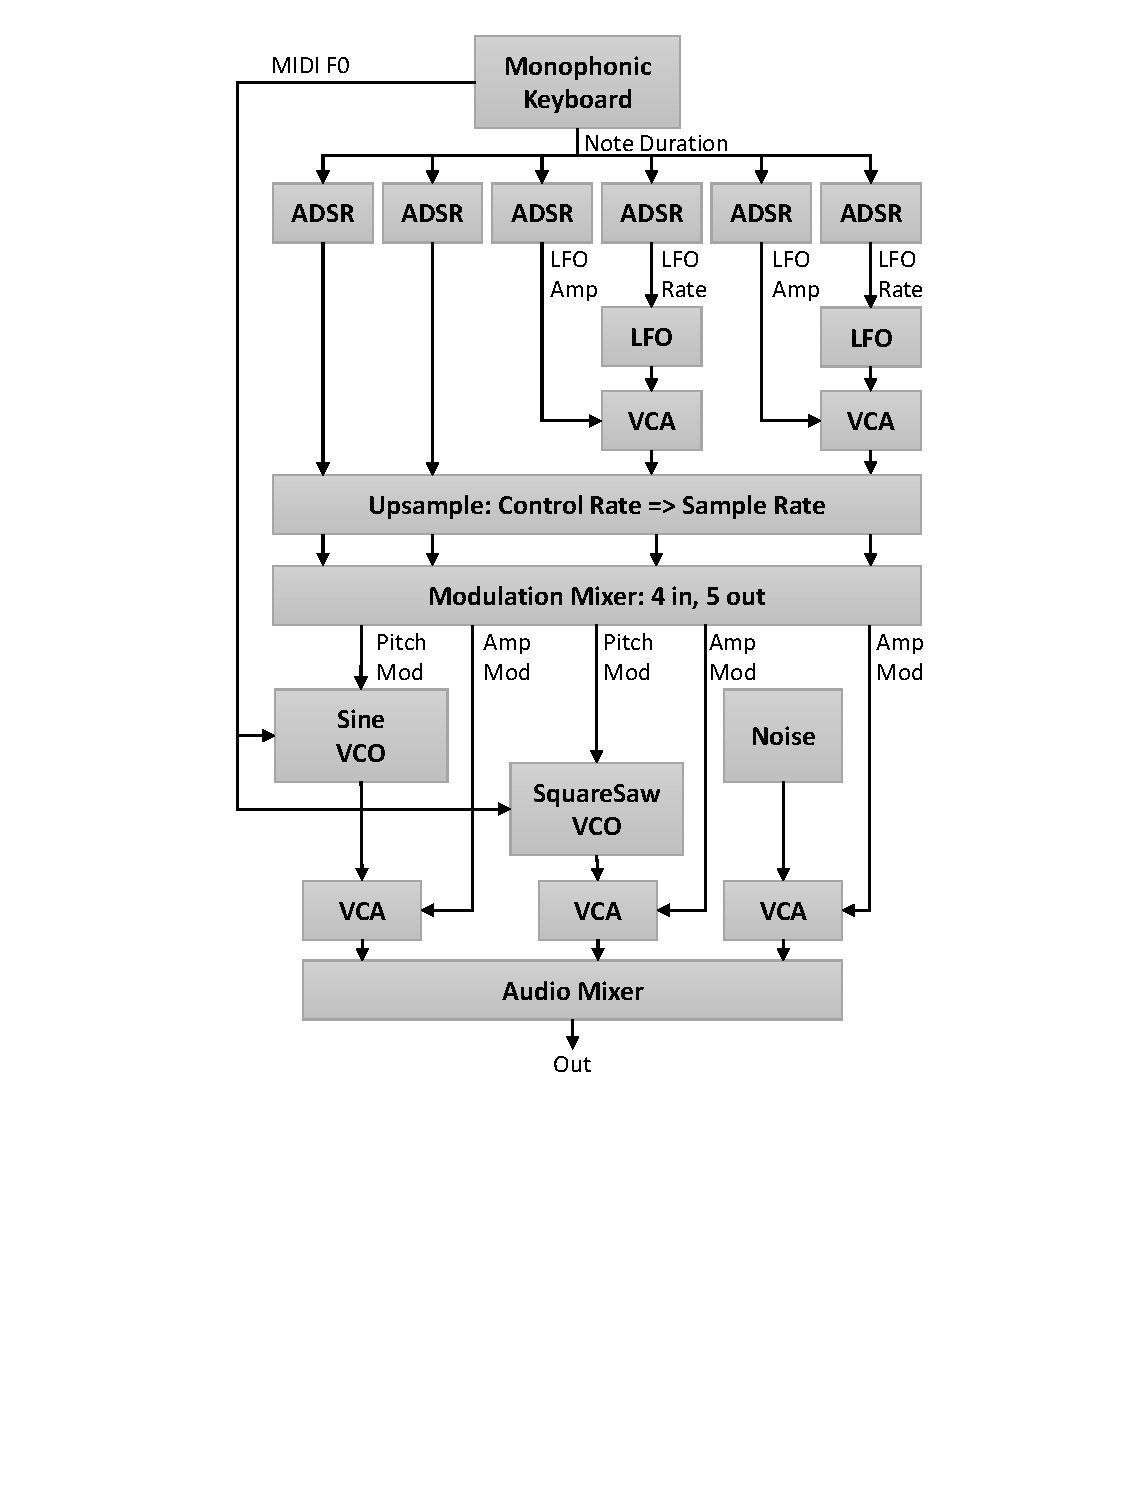
\includegraphics[width=0.6\linewidth]{SynthDiagram_3.pdf}
  \vspace{-1.5em}
    \caption{Module configuration for the Voice in torchsynth}
    \label{fig:voice_diagram}
\end{figure}

%The Voice module is strictly additive and contains no filter.
%Our principle design imperative was fast throughput using traditional synthesis modules, followed by expressivity. Designing fast expressive GPU-enabled filters is an open research question. Infinite Impulse Response (IIR) filters are expressive but require recursive computation, thus impeding computation speed on a GPU \cite{iir}. Kuznetsov {\em et al.}\ \cite{iir} argue that convolution neural networks can be viewed as non-linear Finite Impulse Response (FIR) filters and the promising results of differentiable FIRs used in Engel {\em et al.}\ \cite{engel2020ddsp}
% and Bitton {\em et al.}\ 
%\cite{DBLP:journals/corr/abs-2008-01393} suggest directions for future work. 
While the Voice is the default architecture of torchsynth 1.0, any number of synth architectures can be configured using the available modules. For example, a 4-operator frequency modulation (FM) \cite{chowning1973synthesis} synthesizer inspired by \href{https://www.ableton.com/en/packs/operator/}{Ableton Live's Operator instrument} is currently in development.

\begin{figure}[thb]
    \centering
    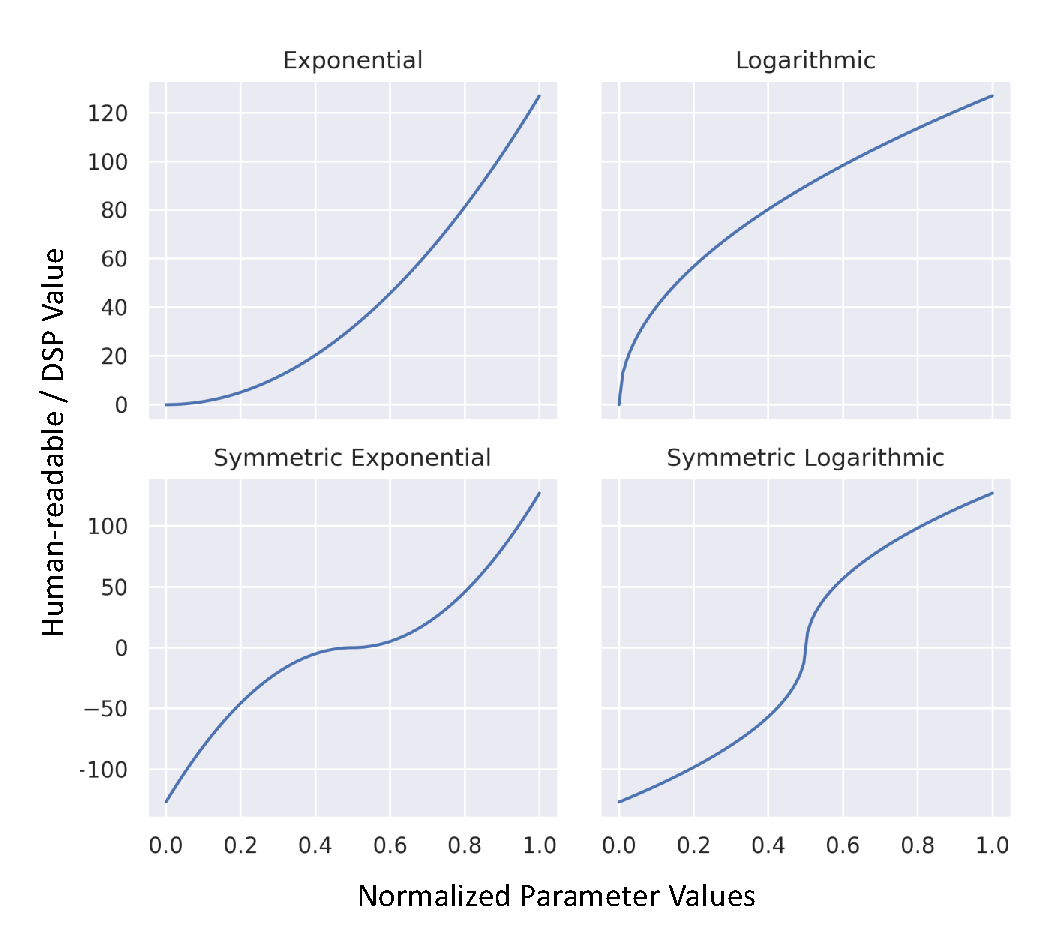
\includegraphics[width=0.80\linewidth]{Hyperparam_4.pdf}
    \caption{Examples of parameter curves used to convert to and from normalized parameter values and the human-readable values used in the DSP algorithms. The top two curves are non-symmetric curves, mapping to values in the range [0, 127]. The bottom two curves are symmetric, mapping to values in the range [-127, 127].}
    \label{fig:parameter_curves}
\end{figure}

\subsection{Parameters}
Module parameters can be expressed in human-readable form with predetermined min and max values, such as $0 \le \textrm{midi f0} \le 127$. These human-intepretable values are used by the DSP algorithms of each module.
Internally, parameters are stored in a corresponding normalized range $[0, 1]$. synth1B1 parameters are sampled uniformly from the normalized range. However, there is potentially a non-linear mapping between the internal range and the human-readable range. Besides the fixed min and max human-readable values, each parameter has hyperparameters ``curve'' and ``symmetry'' that determine how internal [0, 1] values are transformed to the human-readable values. The curve can specify a particular logarithmic, linear, or exponential sampling approach, {\em e.g.}\ to emphasize higher or lower values. Symmetric curves, which alternately emphasize the center or edges of the distribution, are used for parameters such as oscillator tuning where the default value is 0 and can take on a range of both positive and negative values. An example set of non-linear curves is shown in Figure \ref{fig:parameter_curves}.

In our nomenclature, a particular choice of hyperparameter settings, which correspond to random sample space of markedly different sonic character, are called {\em nebulae}. The initial Voice nebula was designed by the authors based upon intuition and prior experience with synthesizers. We experiment with tuning the hyperparameters of Voice to generate different nebulae in \S\ref{sec:hyperparameter-tuning}.

%\subsection{Perceptual motivation for initial hyperparameter choices}

%[ddsp]

%[blah blah blah some of the modules we have implemented]

% [How did we pick the boundaries and scaling]

%[How did we motivate it perceptually]


%\section{Profiling}

%[profile on various GPUs]

%[realtime not throughput]

%[other synths]

%[neural granular synth]

%[speed profiles vs various synths, including wavenets, renderman, surge python, DDSP]

\section{Evaluation of Auditory Distances}

We seek to quantify the diversity of sounds that can be generated with torchsynth, given a particular nebula; or similarly, to quantify to what extent a certain nebula can capture the variability of sounds in another dataset. In order to do so, we first need a reliable measure of similarity or dissimilarity between pairs of sounds, also known as an auditory distance. 

Auditory distances have many applications in audio ML. They provide the basis for quantitative evaluation and optimization criteria. In a sense, the auditory distance measure is the ``ear'' of a model. For example, auditory distances can be used to evaluate the similarity of two sounds that were generated by different synthesis engines. By extension, a well-tuned distance could estimate whether two sounds are perceptually indistinguishable to human listeners. For example, a 4-second sinusoid at 30~kHz, when compared to 4-seconds of silence, should have an auditory distance of zero if the distance is properly tuned to the typical range of human hearing. Likewise, two random instances of white noise should have a perceptual distance of zero, or near zero, despite their entirely different waveforms.

Auditory distances typically involve computing some multidimensional representation of a sound, then computing a distance over the representation space \cite{turian2020im}.
To perform a controlled evaluation of auditory distances, we devised two experiments using two new datasets.
Sounds in each dataset are RMS-level normalized using the \href{https://github.com/kklobe/normalize}{normalize} package.


\begin{table}[ht]
  \centering
  \begin{tabular}{rlcrrrrrr}
{} & & & \multicolumn{3}{c}{Spearman with a preset} & \multicolumn{3}{c}{DCG across presets} \\
 &  &  &  & Surge & DX7 &  & Surge & DX7 \\
Representation & model choice & normed &  & pitch & velocity & mean & &  \\
\hline
OpenL3 \cite{Cramer:LearnMore:ICASSP:19} & env, mel256, 6144  &              &          \textbf{0.821} &           \textbf{0.746} &              0.896 &             0.880 &              0.908 &                 0.852 \\
OpenL3 \cite{Cramer:LearnMore:ICASSP:19}& env, mel256, 6144 & \checkmark     &          \textbf{0.821} &           \textbf{0.747} &              0.895 &             0.809 &              0.883 &                 0.735 \\
OpenL3 \cite{Cramer:LearnMore:ICASSP:19} & music, mel256, 6144 & \checkmark   &          0.817 &           0.732 &              \textbf{0.903} &             0.820 &              0.916 &                 0.724 \\
OpenL3 \cite{Cramer:LearnMore:ICASSP:19} & music, mel256, 6144  &            &          0.813 &           0.722 &              \textbf{0.903} &             0.892 &              \textbf{0.942} &                 0.842 \\
Coala \cite{drossos:icml:2020} & dual\_ae\_c & \checkmark                    &          0.813 &           0.729 &
 0.896 &             0.555 &              0.547 &                 0.564 \\
Coala \cite{drossos:icml:2020} & dual\_e\_c & \checkmark                     &          0.811 &           0.737 &
 0.884 &             0.569 &              0.576 &                 0.563 \\
 
NSynth Wavenet \cite{engel2017neural} & & \checkmark                            &          0.810 &           0.717 &              \textbf{0.903} &             0.582 &              0.591 &                 0.573 \\
OpenL3 \cite{Cramer:LearnMore:ICASSP:19} & music, linear, 6144 &             &          0.808 &           0.722 &              0.895 &             0.874 &              \textbf{0.943} &                 0.805 \\
OpenL3 \cite{Cramer:LearnMore:ICASSP:19} & music, mel256, 512 &              &          0.804 &           0.710 &              0.899 &             \textbf{0.904} &              \textbf{0.943} &                 \textbf{0.864} \\
OpenL3 \cite{Cramer:LearnMore:ICASSP:19} & music, mel256, 512 & \checkmark    &          0.801 &           0.705 &              0.897 &             0.585 &              0.606 &                 0.564 \\
NSynth Wavenet \cite{engel2017neural} & &                                     &          0.789 &           0.675 &              \textbf{0.903} &             0.835 &              0.893 &                 0.777 \\
Coala \cite{drossos:icml:2020} & dual\_ae\_c &                              &          0.776 &           0.658 &              0.893 &             0.748 &              0.756 &                 0.740 \\
Coala \cite{drossos:icml:2020} & dual\_e\_c &                               &          0.750 &           0.630 &
 0.871 &             0.681 &              0.710 &                 0.652 \\
Multi-scale spectrogram \cite{engel2020ddsp,steinmetz2020auraloss} & linear+log, [4096 ... 64] & &          0.792 &           0.690 &              0.894 &             0.543 &              0.555 &                 0.531 \\
Multi-scale spectrogram \cite{engel2020ddsp,steinmetz2020auraloss} & log, [4096 ... 64] & &          0.786 &           0.689 &              0.884 &             0.542 &              0.566 &                 0.518 \\
Multi-scale spectrogram \cite{engel2020ddsp,steinmetz2020auraloss} & linear, [4096 ... 64] & &          0.658 &           0.410 &              \textbf{0.905} &             0.447 &              0.343 &                 0.551 \\
Coala \cite{drossos:icml:2020} & cnn & \checkmark                          &          0.555 &           0.303 &              0.806 &             0.485 &              0.433 &                 0.537 \\
Coala \cite{drossos:icml:2020} & cnn &                                   &          0.552 &           0.297 &              0.807 &             0.714 &              0.614 &                 0.815 \\
 \end{tabular}
  \caption{Performance of representations on experiments defined in \S~\ref{sec:experiment1} and \ref{sec:experiment2}. Best scores, and scores within 0.002 of the best, are bold-faced. $\ell_1$ distance was used because it outperformed $\ell_2$. We sort by mean spearman within a preset.
  }
  \label{tab:distance-eval}
\end{table}


\subsection{DX7 Timbre Dataset}
\label{sec:dx7}

Given 31K unique human-devised presets for the DX7\footnote{We used this clone: \url{github.com/bwhitman/learnfm}}, we generated 4-second samples on a fixed midi pitch (69 = A440) with a note-on duration of 3 seconds. For each preset, we varied only the velocity, from 1--127. This dataset is built on the hypothesis---verified through informal listening tests---that velocity, while carrying no timbral information itself, effects a meaningful, monotonic variation in timbre when it is explicitly programmed into a DX7 patch. Not all DX7 patches are velocity sensitive, and some are more sensitive than others. Sounds that were completely identical---{\em i.e.} each sample matched with error 0---were removed from the dataset. 8K presets had only one unique sound. The median was 51 unique sound per preset, mean 41.9, stddev 27.4.

\subsection{Surge Pitch Dataset}
\label{sec:surge}

The open-source \href{https://surge-synthesizer.github.io/}{Surge synthesizer} is a versatile subtractive synthesizer with a variety of oscillator algorithms: Classic, Sine, Wave-table, Window, FM2, FM3, S\&H Noise and Audio Input. To explore another dimension of variability, in this case {\em pitch}, we used the \href{https://github.com/surge-synthesizer/surge-python}{Surge synthesizer Python API} and the 2.1K standard Surge presets. Here we held the velocity constant at 64, and varied midi pitch values from 21--108, the range of a grand piano. Only a small percentage of presets (like drums and sound effects) had no meaningful pitch variation, and thus no perceptual ordering as pitch increases. However, the inclusion of noise in many of these sounds precluded the use of automatic filtering of perceptually indistinct sounds. Therefore, a small fraction of presets are unclassifiable, imposing a uniform upper bound in accuracy across the board for all auditory distances.
%This small set perceptually unclassifiable was controlled for in our experiments by applying all distances to the exact same presets and sounds, {\em i.e.}\ the small percent of perceptually unrankable presets penalized all distances equally.

\subsection{Distance Experiment 1: Timbral and Pitch Ordering Within a Preset}
\label{sec:experiment1}

In this experiment, we measure the ability of an auditory distance to order sounds by timbre, or by pitch, in the DX7 and Surge datasets, respectively. In effect, the experiment is two evaluations in parallel, run on two separate datasets.

We sample a random preset with at least 3 unique sounds. For each sound $s$, we pick a random sound $s_l$ from this preset with a lower rank (using the DX7 set, this would be a sound having the same pitch but a lower velocity; for the Surge dataset this is a sound having the same velocity but lower pitch); and a random sound $s_h$ with higher rank. %We do not use the min and max rank sounds because they sometimes have unusual timbres, and also to improve experimental control overall. 

For each of $s$, $s_l$ and $s_h$, we compute the distance $d(\cdot, \hat{s})$ between this sound and all other sounds $\hat{s}$ in the dataset. While $s$ is the sample of interest, distance measures are strictly non-negative. Therefore, we seek a concurrent metric to determine whether the compared sound $\hat{s}$ is ``above'' or ``below'' $s$. If the sound $\hat{s}$ is closer to $s_l$, we determine the sign of the distance to $s$ to be negative. If $\hat{s}$ is closer to $s_h$, we determine the sign of the distance to $s$ be positive. As a result, we have a signed distance metric comparing the sound $s$ to every other sound in the dataset.

This set of distances is then correlated to the ground-truth index of pitch, or velocity (depending on the dataset). The correlation, here a Spearman rank correlation, reflects the extent to which the signed distance can properly order the dataset by variability in pitch or velocity. 
One limitation of this methodology for inducing a forced ranking from simple distance is that if, say, $s = 80, s_l = 31, s_h = 81,$ and $\hat{s} = 79$, we might judge $\hat{s}$ as closer to $s_h$ and thus above $s$. We controlled for this by using the same choice for every auditory distance of $s_h$ and $s_l$ given $s$.

Formally, we estimate:
\begin{align}
\begin{split}
\mathop{\mathbb{E}}_{S \in P, s \in S, s_l, s_h \sim S, s_l < s < s_h} \bigg [ \mathop{\rho}_{\hat{s} \in S}\Big (& \textrm{rank}(\hat{s}), d(s, \hat{s}) \ \cdot \\
& \textrm{sgn} \big (d(s_h, \hat{s}) < d(s_l, \hat{s} \big ) \Big) \bigg ]
\end{split}
\end{align}
$P$ is the set of presets, $S$ sounds in that preset, and $\rho$ is spearman.

% Turian adds interstitial magic...

%If $d(s_l, \hat{s}) < d(s_h, \hat{s})$, we negate the distance $-d(s, \hat{s})$ because we assume it is lower rank. Given all distances $d(s, \hat{s})$---some of which are possibly negated---we compute the spearman correlation of the predicted ranks against the true ranks of the sounds within this preset. Spearmans are micro-averaged, i.e., correlations are weighted by the size of constituent presets, over 150 presets, so presets with few timbres are not over-represented.






\subsection{Distance Experiment 2: Determine a Sound's Preset}
\label{sec:experiment2}

A good distance measure should have low distance between sounds generated by the same preset. For each trial, we sample 200 different presets. We sample 2 unique sounds from each preset. For each sound, we compute its distance against the 399 other sounds, and then compute the discounted cumulative gain (DCG) \cite{pmlr-v30-Wang13} of the sound from the same preset, with binary relevance. The DCG is computed for all 400 sounds in the trial. We perform 600 trials.

In the Surge dataset, to control for the helical nature of pitch perception \cite{shepard1982geometrical}, the second sound was always an interval of six semitones (AKA a tritone, {\em diabolus in musica}) from the first note. This ensured that pitches were close, but avoided similar partials due to overlapping harmonics that could be easily matched.

\subsection{Evaluation Results}

To evaluate the perceptual similarity between two audio samples, we need a good representation to compute distances: a) The multi-scale spectrogram distance has been used in a variety of applications, particularly in speech synthesis \cite{wang_neural_2019,DBLP:conf/icassp/YamamotoSK20} but also in music \cite{DBLP:journals/corr/abs-2008-01393,engel2020ddsp,dhariwal2020jukebox};
b) NSynth Wavenet \cite{engel2017neural} is a Wavenet-architecture trained on NSynth musical notes; c) OpenL3 \cite{Cramer:LearnMore:ICASSP:19} was  trained multi-modally on AudioSet audio and video, on two distinct subsets: music and environmental sounds; d) Coala \cite{drossos:icml:2020} was trained multi-modally on Freesound audio and their corresponding tags.

We experimented with a variety of hyperparameter settings for the representations. The best results are in Table~\ref{tab:distance-eval}. $\ell_1$ distance was used because it gave better results than $\ell_2$ across the board. For Coala and NSynth Wavenet, normalizing
% We maybe should have done l1 norm not l2 norm :\
improves the spearman scores, but harms the DCG across presets. Normalization had little effect on OpenL3. %Although the Spearman tasks are the most difficult,
OpenL3 (music, mel256, 512) achieves the best score on DCG across presets, and its compactness makes it an appealing choice for the remaining experiments in the paper.

\section{Similarity between Audio Datasets}
\label{sec:similarity-dataset}

To evaluate the similarity between two sets of audio samples $X$ and $Y$, we use the maximum mean discrepancy (MMD) \cite{JMLR:v13:gretton12a}. We use the following MMD formulation, assuming $X$ and $Y$ both have $n$ elements:
% One thing that's weird is you always get negative numbers and they do sqrt
\begin{equation}
    \textrm{MMD}(X, Y) = \frac{1}{n n} \sum_{i,j=0}^n 2 \cdot d(x_i, y_j) - d(x_i, x_j) - d(y_i, y_j)
  \label{eq:mmd}
\end{equation}
MMD allows us to use our chosen distance measure---OpenL3 (music, mel256, 512) $\ell_1$---as the core distance $d$.

\iffalse
\begin{equation}
  \begin{aligned}
    \textrm{MMD}(X, Y) = - \frac{1}{m m} & \sum_{i,j=0}^m d(x_i, x_j) \\
    -  \frac{1}{n n} & \sum_{i,j=0}^n d(y_i, y_j) \\
    + \frac{2}{n m} & \sum_{i,j=0}^{m,n} d(x_i, y_j) \\
  \end{aligned}
  \label{eq:mmd}
\end{equation}
\fi

% We should re-run this with the new noise setting

\begin{table}[th]
    \centering
    \begin{tabular}{r|r|ll}
MMD & std & corpus 1 & corpus 2 \\
\hline
4.396 & 0.123 & white & white \\
21.409 & 4.729 & dx7 & dx7 \\
23.732 & 3.615 & FSD50K & FSD50K \\
24.130 & 5.251 & torchsynth & torchsynth \\
27.824 & 9.821 & surge & surge \\
2751.519 & 80.955 & torchsynth & surge \\
2884.843 & 67.264 & surge & dx7 \\
3001.857 & 71.888 & torchsynth & FSD50K \\
3637.845 & 79.265 & torchsynth & dx7 \\
4756.952 & 112.705 & surge & FSD50K \\
7413.105 & 111.897 & dx7 & FSD50K \\
13202.202 & 61.558 & white & FSD50K \\
16985.319 & 92.992 & white & torchsynth \\
18488.926 & 67.277 & white & surge \\
20374.929 & 78.886 & white & dx7 \\
\end{tabular}
    \caption{MMD results comparing different audio sets, including the stddev of the MMD over the 1000 trials.}
    \label{tbl:corpora-mmd}
\end{table}

\iffalse
\begin{table}[ht]
    \centering
    \begin{tabular}{r|r|ll}
MMD & std & corpus 1 & corpus 2 \\
\hline
75.631 & 1.032 & white & white \\
242.773 & 53.653 & dx7 & dx7 \\
270.787 & 37.008 & FSD50K & FSD50K \\
279.554 & 85.973 & surge & surge \\
285.322 & 64.507 & torchsynth & torchsynth \\
18935.366 & 498.315 & torchsynth & surge \\
23621.233 & 643.370 & surge & dx7 \\
27763.655 & 699.799 & torchsynth & dx7 \\
32907.268 & 875.941 & torchsynth & FSD50K \\
37907.643 & 891.741 & surge & FSD50K \\
68831.634 & 1071.538 & dx7 & FSD50K \\
134643.313 & 988.875 & white & FSD50K \\
189336.626 & 1406.814 & white & torchsynth \\
190260.499 & 945.127 & white & surge \\
234607.035 & 1155.182 & white & dx7 \\
\end{tabular}
    \caption{env mel256 6144}
    \label{tbl:corpora-mmd2}
\end{table}
\fi


\iffalse
\begin{table}[ht]
    \centering
    \begin{tabular}{r|ll}
MMD & corpus 1 & corpus 2 \\
\hline
4.477 & white & white \\
17.607 & DX7 & DX7 \\
18.229 & Surge & Surge \\
26.438 & FSD50K & FSD50K \\
2847.637 & Surge & DX7 \\
4692.223 & Surge & FSD50K \\
7303.703 & DX7 & FSD50K \\
13257.964 & white & FSD50K \\
18540.486 & white & Surge \\
20266.055 & white & DX7 \\
\end{tabular}
    \caption{MMD results comparing different audio sets.}
    \label{tbl:corpora-mmd}
\end{table}
\fi


For Surge and DX7, we selected sounds with midi pitch 69 and velocity 64. We also generated a set of 4-second samples of white-noise, and used excerpts from the FSD50K evaluation set \cite{fonseca2020fsd50k}, which is broad-domain audio, trimmed to 4 seconds. From each corpus, we randomly sampled 2000 sounds, to match the size of the smallest corpus (Surge). We performed 1000 MMD trials, each time comparing $n=1000$ sounds from one corpus to $n=1000$ sounds from another,  randomly sampled each trial. To estimate the diversity within a particular corpus, we evaluated MMD over 1000 distinct 50/50 partitions of the corpus.

Table~\ref{tbl:corpora-mmd} shows the result of average MMD computations between different audio corpora. 0.0 would be perfectly identical. Some results are expected, whereas some are counter-intuitive and suggest pathologies in the OpenL3 distance measure. These results are sometimes perceptually incoherent, and suggest that existing auditory distance measures will impede progress in automatic synthesizer design, as we will illustrate in the following section.


\begin{itemize}
    \item White-noise is the most similar to itself of all comparisons.
    \item FSD50K broad-domain sounds are, strangely, considered to have less within-corpus diversity than torchsynth or Surge sounds. However, the variance is high enough that it is hard to have statistical confidence in this unexpected result.
    \item More troubling are low-variance estimates that torchsynth is more similar to FSD50k than a dx7 synth. {\em A priori}, one would expect that synths would sound more similar to each other than broad domain audio. %Perhaps this is because dx7 contains no noise, whereas FSD50K and torchsynth do. (However, then dx7 and surge should not be more similar.)
    \item As expected, white noise is the least similar to DX7 synth sounds of all corpora, as the DX7 has no noise oscillator.
\end{itemize}



\section{torchsynth Hyper-Parameter Tuning}
\label{sec:hyperparameter-tuning}

Given its highly flexible architecture, how can we guarantee the maximum diversity of sounds within the default nebula? Similarly, to what extent can torchsynth adopt the characteristics of a given corpus of audio? Recall from \S\ref{sec:design-methodology} and Figure~\ref{fig:parameter_curves} that for each module parameter, the choice of scaling curve is a hyperparameter. Initial hyperparameters were chosen perceptually and based upon prior-knowledge of typical synth design.

In principle, we can use MMD (Equation~\ref{eq:mmd}) as an optimization criterion to tune these hyperparameters a) to maximize sonic diversity; or b) model the characteristics of another dataset. We use Optuna \cite{optuna_2019}, initializing with 200 random grid-search trials, and subsequently using CMA-ES sampling for 800 trials. In each trial, we generate 256 random torchsynth sounds with the Optuna-chosen hyperparameters. %, and computed the averaged MMD over 1000 50/50 splits of the sounds.
Hyperameter curves were sampled log-uniform in the range [0.1, 10]. The top 25 candidates were re-evaluated using 30 different MMD trials, to pick the best hyperparameters. However, MMD estimates are only as good as the underlying similarity metric (OpenL3-$\ell_1$) that it uses.
% try GPyOpt?

For these experiments, the authors and non-author musicians conducted blinded listening experiments of the tuned nebula and our manually-chosen nebula, and listened to 64 random sounds. Only after independent qualitative evaluation did we unblind which nebula was which.

\iffalse
\subsubsection{Quantifying perceptual redundancy in synth1B1}

The further quantify potential redundancy in the final synth1B1, we ran the following experiments:
\begin{itemize}
\item Using OpenL3-$\ell_1$-distance distributions of synth1K1, synth10K1, and synth100K1, we estimate the OpenL3-distance distribution for a random synth1B1 sound as [figure]
\item Using Amazon Mechnical Turk, we ran ``just-noticeable-differences'' experiments between pairs of synth1B1 samples with particular OpenL3 distance \cite{Manocha:2020:ADP}. This allows us to estimate, for a particular OpenL3 distance, what the likelihood is that the sounds are perceptually indistinct.
\item Combining these two estimates, we believe that [...]\% of sounds in synth1B1 are perceptually distinct.
\end{itemize}
\fi

\subsection{Restricting hyperparameters}

%A hyperparameter subset that reduces diversity but has certain desirable qualities, we call a nebula. %For example, we are curious if we can discover the Moog nebula. We present two experiments in minimizing OpenL3-MMD against existing sound corpora.
%In future work, we are interested to push this approach further and explore the synth1B universe of sounds.

\iffalse
\subsubsection{Mimicking ``natural'' synthesis}

Recall that our DX7 (\S\ref{sec:dx7}) and Surge (\S\ref{sec:surge}) corpora are based upon ``natural'' synthesized sounds, i.e.\ presets designed by humans. This choice stands in contrast to similar work in which synthesizer presets are generated at random.

torchsynth 1.0 Voice's synthesis approach is more similar to Surge's than DX7.\footnote{Stay tuned for torchsynth 2.0 which will have a DX7 style FM synth}
To mimic Surge's human-curated presets, we tune our hyperparameters to minimize the MMD between torchsynth Voice and Surge. [results]

\subsubsection{Mimicking percussive sounds}
\fi

Many torchsynth 1.0 Voice default nebula sounds have an eerie sci-fi feel to them.
To find the drum nebula, we used Optuna to choose hyperparameters to {\em minimize} the OpenL3-$\ell_1$-MMD against 10K one-shot percussive sounds \cite{ramires2020}. All hyperparameters were allowed to be tuned.
%Note that we listened to the drum-restricted synth sounds blindly, so we took qualitative notes on standard torchsynth and Optuna-drum-tuned torchsynth simultaneously, knowing only the different experimental conditions.
We had hoped to find that OpenL3-$\ell_1$-MMD would find appropriate percussive curves.

Overall, we found the drum hyperparameters unpleasant to listen to. This negative result was surprising. Sounds did not resemble percussion. There was extreme use of high and low pitch. Low pitches were clicky and gurgly, high pitches were painful or often inaudible. There was some nice use of LFO, but little use of square shape, little noise, and low diversity. Perhaps wide modulation sweeps attempted to compensate for the broadband energy in the transients of drum sounds.

We were curious if this negative result was due to failure of the distance measure, or instead a systemic limitation in the design of the torchsynth 1.0 Voice and its parameter sampling approach. We hand-tuned the hyperparameters to create a drum nebula, which is shared as part of our repository. While not all the sounds produced sound like drum hits, many have a quality akin to early drum machines---the distribution of sounds is overall much more percussion-like. We encourage the reader to listen to this nebula, which will be available on torchsynth site.

In addition to confirming the perceptual-deafness of our distance measure, hand-designing the drum nebula demonstrated one limitation in torchsynth 1.0: Synth parameters are all sampled independently. Thus, one cannot construct a nebula that samples only kicks and snares. Sampling occurs on the continuum between them. In future work, we are interested in investigating multivariate sampling techniques, which would allow more focused cross-parameter modal sound sampling.

\subsection{Maximizing torchsynth diversity}
\label{sec:diversity}

We attempted to tune our hyperparameters to maximize torchsynth MMD, i.e.\ increase the perceptual diversity of sounds generated by torchsynth itself. As before, Optuna was used to choose hyperparameters that maximized the OpenL3-$\ell_1$-MMD and thus increase the diversity of sounds. Nonetheless, the ``optimized'' nebula exhibited pathologies in pitch, favoring extremely low and high pitches. We hypothesize that OpenL3-$\ell_1$ overestimates perceptually diversity in these frequency ranges. We performed numerous experiments restricting the hyperparameters Optuna could and could not modify, such as prohibiting changes to midi f0 and VCO tuning and mod depth. Consistently, listeners preferred our manually design nebula to automatically designed ones in blind tests. We consider this another important negative result. Open questions remain:
\begin{itemize}
    \item For what hyperparameter choices is a particular auditory distance perceptually-inaccurate?
    \item How do we craft an auditory distance measure that can {\em perceptually} optimize synthesizer diversity, or similarity to an existing sound corpus?
\end{itemize} 

\iffalse

In initial experiments, we allowed every hyperparameter to be varied. Preliminary listening tests had indicated that the ``tuned'' diverse synth had a sharp f0 curve, favoring extremely low and high pitches. We hypothesize that OpenL3 overestimates perceptually diversity in these frequency ranges. Thus, for the rest of this experiment we froze f0 at 69 and note-on duration at 3 seconds as in \S\ref{sec:similarity-dataset}. (torchsynth 1.0 does not have a velocity parameter.) We also froze the VCO's mod-depth and tunings to hand-selected torch defaults.

Nonetheless, blinded experiments by the authors found the OpenL3-diversity-maximized synthesizers exhibited a variety of pathologies, and were unsuitable for release. Thus, synth1B1 (and torchsynth 1.0's default hyperparameters) are the ones originally chosen by the authors based upon perceptual experiments and expert knowledge. 
\fi

\iffalse
We hoped then that OpenL3 MMD's would nonetheless diversify the synth's timbre and time-frequency elements.

In our final qualitative diversity experiments, we had three synths: torchsynth with manually-chosen hyperparameters, torchsynth optimizing OpenL3-music-mel256-512 MMD, and torchsynth optimizing OpenL3-music-linear-512 MMD (with hyperparameters frozen as above). At listening time, we used midi f0 69.

The blinded qualitative evaluation by the authors revealed the following. The results are ordered from our least favorite through most favorite:

\begin{description}
\item[OpenL3 mel256] Not very diverse. Sounds tended to be short and percussive, with little variation in amplitude attack, with a lot of ``ping'' and ``ting'' sounds. Nonetheless, the only variation we heard with short sounds. There was some ringing. There not a full use of the sonic range, typically one oscillator coupled with one modulated, one non-moving pitch, and little warble. More noise burst sounds.
\item[OpenL3 linear] Overall, the most monotonous and static, with the least rhythmic diversity. Had many extreme pitch variations and was ``sireny'', appearing to have less intent and uselessly random extreme pitch modulations. Despite using f0 69 and our hand-tuned VCO mod depth and tuning, the automatically-tuned modulation mixer could be routing a lot of modulation to the pitch.
It was poorly balanced for loudness, perhaps due to the amplitude normalization and low energy.
The envelopes tend to have shorter attacks.
Aggressive sounding.
\item[Manually tuned] A good mix of stationary and modulated sounds. Good ``sci-fi'' sound effects. Focused more on sound effects than ``musical'' instruments, due to strong use of diverse pitch modulation. Well-behaved pitch and use of the range. Balanced mix of noisy and clean sounds, perhaps slightly too high of a consistent noise floor.
\end{description}
We discuss these issues in more depth in \S\ref{sec:issues}.
\fi


\iffalse
\section{Possible Benchmarks}

To demonstrate how synth1B1 might be used, we measure baselines on two fundamental tasks. These experiments are not meant to limit the applicability of our work, but rather to provide simple examples of how they might be used to understand fundamental challenges in audio ML.

% Again, I want to reiterate that 1B might make it easy to memorize this task and we might want to try on 1M etc

\subsection{Task 1: Audio Difference Perceptability}

% MH: This is a toy example of what can be done with the dataset.
% goal 1: distance measure (a single scalar (?))

Our first benchmark task is evaluating whether an auditory distance correlates with human perception. Loss functions that involve audio-to-audio distance are pervasive in the literature, but common differentiable auditory distance measures are poorly correlated with human perception.

The task is as follows: Given the training set, impute a binary classifier that determines whether a human would perceive two audio samples as the same or not (``just noticeable differences''). The objective is to maximize accuracy [FMS?] on the test set.

Here is our baseline: The current state-of-the-art auditory distance measure is the multi-scale spectrum distance. We use the standard parameters given in [....]. We determine the threshold of perceptibility in the multi-scale spectral distance using human trials, based upon pairs in the training set. Using this threshold, we predict audio difference perceptibility on the test set. For varying sizes of the training data, our accuracy [FMS] is show in table [...]

[auraloss?]

% TODO: Run this


\subsection{Task 2: Inverse Synthesis}

Synthesizers have become ubiquitous in music, sound design, and text-to-speech systems since their inception. Despite their widespread use, synthesizers generally have large parameter spaces with non-linear and complex parameter interactions that require specific technical knowledge to make effective use of. One of the most commercially successful music synthesizers, the Yamaha DX7, was notoriously challenging to program; ``allegedly, nine out of ten DX7s coming into workshops for servicing still had their factory presets intact'' \cite{ seago2004critical}. A recent survey of synthesizer users’ confirmed a desire amongst participants for more intuitive systems for interacting with these devices \cite{krekovic2019insights}. This desire is reinforced by the body of research focused on the development of more alternative methods for programming synthesizers as well as the burgeoning field of neural audio synthesis. 

The general problem of inverse synthesis is as follows: given an audio sample, infer the latent space of synthesis parameters used to generate this sound. This task is confounded by the fact that there is a many-to-one relationship between parameters and the synthesized sound. Additionally, measuring error in the parameter space might not correspond to true perceptual distance between two sounds. Thus, we evaluate the inferred parameters for a given test sound by re-synthesizing those parameters, and have humans evaluate if there is a perceptible difference between the target test audio and predicted test audio.

% Do we need to describe the experimental methodology of JND here??

Again, our na\"{i}ve baseline is based upon the multi-scale spectral loss: For a given test audio samples, represent it using the multi-scale spectral loss. Find the one-nearest train audio sample. [l2? of multiscale] Use that 1NN training audio's parameters to synthesize the predicted test audio. Results are presented below:
% TODO: Run this with various sizes, synth1M1 and synth100K1??

% And maybe a 10NN average

\subsection{Discussion of Benchmarks}

Again, we reiterate that we demonstrate simple baselines for future researchers. Another important application is transfer learning, where audio representations are learned over synth1B1 and then used to fine-tune smaller corpora.
\fi


\section{Open Questions, Issues, and Future Work}
\label{sec:issues}

%\subsection{Issues with the distance}

Many experiments in automatic synthesizer design hinge on having a perceptually-relevant auditory distance measure. The distance measure is the artificial ``ear'' of the network.
OpenL3 (music, mel256, 512) $\ell_1$ performed well on our quantitative synthesizer experiments (Table~\ref{tab:distance-eval}), but exhibited many issues in qualitative listening tests, in particular its insensitivity to extreme pitch and inability to model percussion.

Learning a perceptually-relevant auditory distance measure is an open research question. Manocha {\em et al.}\ \cite{Manocha:2020:ADP} use manually-annotated ``just noticeable differences'' (JND) trials generated using active learning to induce a perceptual distance measures. However, they only work with speech and do not include pitch variations, so their model was inappropriate for our task.

Unknown pathologies in auditory distance measures impede researchers from performing a variety of useful experiments. Most crucially, the lack of perceptually accurate auditory distance measure prevented us from precisely estimating how many perceptually different sounds are expressible by torchsynth, as well as other synthesizers like Surge and DX7. By contrast, a good artificial ``ear'' for music opens the door to many possible advances in synthesizer design, including:
\begin{itemize}
    \item Estimating and maximizing the diversity of synthesizer.
    \item Mimicking existing synthesizers through automation.
    \item Inverse synthesis, transcription, and the other tasks described in \S\ref{sec:contributions}. 
\end{itemize}
Our negative results on automatic synthesizer design using auditory distances present valuable challenges for the community to investigate.

Nonetheless, the potential impact (\S\ref{sec:intro} and \S\ref{sec:contributions}) of the synth1B1 corpus is unaffected, because of its enormous size, speed, and corresponding multi-modal latent parameters.

%Another possible criticism of our qualitative evaluation of synth diversity is that the authors' prior experience with synthesizers led us to prefer sounds to which we are accustomed, rather than those that are maximally perceptually diverse. Again, this underscores the need for an automatic audio distance measures that is perceptual and can accurately measure just-noticeable-differences in synthesized sound.


\iffalse
\subsection{Hyperparameter choices}

Overall, we were surprised at the inability of OpenL3-MMD to mimic percussion sounds.

Nonetheless, it is also possible that our hyperparameter curves (which are either linear, logarithmic, exponential, or S-shaped) should be include other options. In future work, we can attempt to devise the drum nebula by hand, in order to determine if there is an intrinsic limitation in torchsynth 1.0 at modeling percussion.

A possible additional limitation of torchsynth 1.0's hyperparameters is that parameter minimum and maximum values are fixed (hyperhyperparameters). For example, the ADSR attack ranges from 0.0--2.0 seconds, and the hyperparameter curves only determine the sampling probability distribution within this range. It's possible that allowing these min and max values to vary would allow for greater flexibility.
\fi

\section{Future Work}

torchsynth 1.0 focuses on high throughput and creating a (subjectively) perceptually diverse synth1B1 dataset. %Besides the issues discussed in \S\ref{sec:issues}, 
There are a handful of improvements we want to add to torchsynth:
\begin{itemize}
\item Stress-tested differentiable modules.
\item Subtractive filters.
\item Additional architectures including an FM synthesizer.
\item Multivariate parameter selection.
\item High-throughput modules that resemble human speech.
\item A standardized modular architecture for high-throughput audio {\em effect} research.
\end{itemize}

%[all the dafx stuff on fx, DPAM work]

\section{Conclusions}

We release synth1B1, a multi-modal corpus of synthesizer sounds with their corresponding latent parameters, generated on-the-fly 16200x faster than realtime on a single V100 GPU. This corpus is 100x bigger than any audio corpus present in the literature. Accompanying this dataset is the open-source modular GPU-optional torchsynth package. We hope that larger-scale multi-modal training will help audio ML accrete the benefits demonstrated by previous NLP and vision breakthroughs.

We freely release pitch and timbre datasets based upon ``natural'' synthesis sounds, and novel evaluation tasks on which we benchmark a handful of audio representations. We present several novel research questions, including how to estimate and maximize the diversity of a synthesizer, as well as how to mimic existing synthesizers. We outline issues and open research questions that currently impede this sort of experimental work, in particular demonstrating negative results of auditory distance measures.

%Many thanks to the great number of anonymous reviewers.

%[other people who gave us feedback: Esling, Adrien, etc.]

%\newpage

\iffalse
Other stuff to add:

* 1d navigation
* Principle curve: https://pypi.org/project/prinpy/ (https://web.stanford.edu/~hastie/Papers/Principal_Curves.pdf)
\fi

%\nocite{*}
%\bibliographystyle{IEEEbib}
%\bibliography{ddsp}

\iffalse
\section{Appendix}

\section{Other stuff to cite maybe}

% Learning images from synthetic weakly related data:
% Playing for Data: Ground Truth from Computer Games
% The SYNTHIA Dataset: A Large Collection of Synthetic Images for Semantic Segmentation of Urban Scenes
% Learning Aligned Cross-Modal Representations from Weakly Aligned Data


% Wessel DL. Timbre space as a musical control structure. Computer music journal. 1979 Jun 1:45-52.

% Perceptual scaling of synthesized musical timbres: Common dimensions, specificities, and latent subject classes

% Automatic Synthetizer Preset Generation with PresetGen



Jesse Engel DDSP Paper \cite{engel2020ddsp}
Vapar synth-a variational parametric model for audio synthesis \cite{subramani2020vapar}

Timbre space representation of a substractive synthesizer \cite{vahidi2020timbre}

Multi-spectral loss \cite{wang2019neural}

DrumGAN \cite{nistal2020drumgan}

https://ieeexplore.ieee.org/document/7471749

CDPAM: CONTRASTIVE LEARNING FOR PERCEPTUAL AUDIO SIMILARITY

COLA

Citations in secret sauce synth blog posts

SimCo, etc correspondence on vision.

\section{Rock `n Roll: What is it, and how is it affecting our children?}

Evaluation task with NNs: Many-to-one from parameters to audio. Given parameters, predict audio. Mean reciprocal ranks. Or PRC@k where k is 5 or 100.

IIR it's slow and these guys saw that too.

Might also be cool to compare download speeds to generation speeds.

%To avoid these confounding issues, we formulate our problem as pure representation learning as follows: For a given synth parameter set in the test set, rank the test audio according to its likelihood to correspond to this parameter set. We measure the model based upon NDCG [MRR?]. The training set can be used to learn the model, but no information about {\tt torchsynth}'s modular DSP architecture can be used in the model. That is, the contrastive representation leaning task should be approached in a black box manner.

The use of machine learning to help in the process of synthesizing new audio has evolved along two paths: one approach has sought to learn parameters for traditional synthesis algorithms such as Frequency Modulation (FM) and Wavetable synthesis, whereas neural synthesis has leveraged advancements in deep learning to synthesize audio directly within neural networks. Work that follows the first approach, which falls under the umbrella of automatic synthesizer programming, typically has the goal of finding parameter settings to match a given audio input. The benefit of this is that these methods can potentially be used on commercially available synthesizers and also acknowledge the fact that synthesizer users enjoy the process of turning knobs and tweaking parameters – something that they can still do after the machine learning algorithm has produced a parameter selection. 
\fi

	\graphicspath{{./}{./figures/}{./figures/synthexplore/}}

% Principle curve stuff could be neat
% \iffalse
% Other stuff to add:

% * 1d navigation
% * Principle curve: https://pypi.org/project/prinpy/ (https://web.stanford.edu/~hastie/Papers/Principal_Curves.pdf)
% \fi


\chapter{Designing a Synthesizer Programming Interface}
\label{ch:visualization}
In this chapter I introduce Synth Explorer, a prototype of an automatic synthesizer programming interface built on top of the torchsynth synthesizer. Synth Explorer is an interactive visual browsing interface for torchsynth that was built with goal of supporting both novice and expert users in the process of navigating and developing an understanding of the vast and complex sonic space expressed by a synthesizer. It builds upon previous research in the area of sound visualization and the design is informed by concepts from the the fields of creativity support tools (CSTs) and music interaction [need cites]. These concepts, along with the taxonomy of automatic synthesizer programming interaction approaches presented in \S\ref{chapter:asp-background} grounds the the development of Synth Explorer, and provides a framework for the development of future systems. %Synth Explorer is an example of an exploratory interface, with potential for inclusion of additional interaction style, such as an example-based interface. I hope that this 

Synth Explorer is designed with music producers, audio practitioners, and synthesizer users in mind; individuals who regularly require synthesized sounds for their creative projects. These users currently must either manually program a sound, find an existing preset, or find a pre-existing sound in a collection of samples. Challenges with manually programming sounds has already been addressed in detail in chapter \S\ref{chapter:background}. Searching for presets and pre-existing sounds typically involves browsing through items that are displayed in a list-based user-interface and any searching is based on filenames or semantic tagging \cite{knees2016searching}. In conversations held by Kristena Andersen at the RedBull Music Academy \cite{andersen2016conversations}, music producers expressed the challenges associated with navigating large collections of audio and their desires for improved methods for interaction. A particular emphasis was placed on the role of the potential impact of tools that aid the creative process as opposed to taking over. The field of creative music information retrieval has also had the focus of finding ways to address the challenges of searching for sounds \cite{humphrey2013brief} and visual browsing interfaces have been identified as beneficial for allowing users to navigate large collections of sounds more efficiently than traditional list based methods \cite{turquois2016exploring}.

The interface implemented in Synth Explorer is intended to support the efficient navigation of synthesizer sounds, allowing users to develop a "sound palette" for their project. Users are able to "look under the hood" of the visual interface and directly interact with the underlying control interface for these sounds. They can make fine adjustments to the parameter settings to refine their selected sounds as well as to gain insight into the parameter settings that lead to the resulting sound. In this way, users can interact with the synthesis engine and control interface at a level abstraction that supports their position on the learning curve. The graphical interface is designed to support novice users. While the interface includes some technical audio terms, the drag and drop interface is modelled off of an interaction modality that will be familiar to most computer users and will allow anyone to quickly start constructing visualizations and exploring sounds. The inclusion of the technical names will allow users to begin to build up an understanding of the different dimensions of sound and how they relate to the underlying synthesizer parameters.

\section{Related Work}

Exploration-based interfaces for synthesizers was reviewed in chapter \S\ref{chapter:asp-background} and visualization of sounds based on sound similarity has been studied in depth and is reviewed by Cooper \textit{et al.} \cite{cooper2006visualization}. Within the field of automatic synthesizer programming, Synth Explorer is related to the data-driven approach used by in SynthAssist \cite{cartwright2014synthassist}; all the sounds used in Synth Explorer are pre-computed and audio features are stored in a database. Synth sounds are then displayed on the interface based on sound similarity. Looking beyond synthesizer sounds, work that is particularly relevant to Synth Explorer is DrumSpace, a 2D visualization interface developed by Turqois \textit{et al.} for exploring large collections of drum sounds \cite{turquois2016exploring}. A component of their study was a subjective evaluation that compared user experiences in browsing for drum sounds using a traditional list-based layout of samples to 2D visual layouts. For the 2D layouts they compared one method that automatically sorted sounds based on sound similarity against one that organized sounds based on the filename. Users reported having a significant preference for for the 2D based layout, but had no significant preference for the type of layout. Participants were able to explore a much larger number of audio examples in a shorter period of time when using the 2D interfaces. Turqois \textit{et al.} also identified that the layout based on sound similarity caused some confusion to the users; the layout was based on a set of audio features which had been reduced to 2D using a dimensionality reduction technique called t-SNE \cite{van2008visualizing}, because algorithms like t-SNE create complex combinations of higher dimensional features into a lower dimensional embedding for visualization, the meaning of the resulting dimensions used for visualization are often hard to identify. Turqois \textit{ et al.} also suggest that color could be a helpful addition to the interface. Building upon this work, my supervisors and I conducted further experiments on the perceptual relevance of different methods of dimensionality reduction techniques for visualizing drum samples in 2D and identified MDS as having the highest correlation with user similarity ranking \cite{shier2021manifold}. Synth Explorer builds on these tools and leverages similar techniques for creating 2D visualizations of synthesizer sounds.

An interesting CST that is related to the audio synthesis problem is a tool developed by Andrews for exploring and generating graphics using a 2D interface \cite{10.1145/3325480.3325506}. Their work used an algorithmic method for generating 2D graphics, which a user is able to interact with to control the generation of new graphics. Because of the vastness of the space of potential images that could be generated by the algorithm, the user interface utilizes a spatial layout of images to allow the user to quickly assess a set of possibilities which they can then use to guide the generation of further images. While this interface was focused on the generation of images, the interaction ideology is similar to that of Synth Explorer, which is built on top of an algorithmic audio synthesis engine; the space of possible sounds that a synthesizer can produce is far too vast for a user to navigate all at once, so a small random subset of that space is initially presented and the user is then able add more sounds and hone in on a particular result.

\section{Design Principles}
In this secion I present an overview of design principles, informed by the HCI fields of music interaction and creativity support, that are intended to guide the development of automatic synthesizer programming interfaces. These principles provide a framework for designing interactions from the perspective that a synthesizer is a musical tool that users \textit{want} to engage with in the context of a creative pursuit, whether that is designing sounds for a film soundtrack, composing a piece of electronic music, or simply enjoying creating sounds and playing a synthesizer. Because of the breadth of what a creative pursuit can encompass, these principles are intended to be taken as suggestions to help situate the design process.

\subsection{Music Interaction}
Music and Human-Computer Interaction \cite{holland2013music}, or simply Music Interaction, is the field of research related to the use of interactive systems that involve computers for any kind of musical activity. Music interaction draws heavily from other areas of HCI research, but also responds to the needs and desires of the music community. There are unique considerations that makes music interaction different from other fields of HCI. A musical instrument is not a utilitarian tool whose development should be ever-improved and made more efficient. Musical instruments are played, and sometimes that is the only goal. Tomaka [cite me!] identifies that imperfections and limitations of a musical instrument give an instrument character. This was reflected by music producers interviewed by Andersen who expressed the role of serendipity and "happy accidents" in their creative process \cite{andersen2016conversations}, and identified this as an important consideration for designing new music production tools. McDermott \cite{mcdermott2013should} identifies the importance of engagement in musical interaction and the relation that bears to the concept of \textit{flow} \cite{csikszentmihalyi1990flow}. The role that the learning curve plays is crucial to the level of engagement that a player experiences when playing a musical instrument, both in the short-term and long-term. Holland \cite{holland2013music} concludes, "In order to remain engaging, consuming and flow-like, activities that involve musical instruments must offer continued challenges at appropriate levels of difficulty: not too difficult, and not too easy." 

Automatic synthesizer programming tools can be thought of as being extensions of a musical instrument. With this in mind, the goal should not necessarily be to provide a perfectly optimized experience that completely takes over the task of programming and using a synthesizer. For example, example-based inverse synthesis approaches may play an important role in an automatic synthesizer programming tool, however, they may only be one part of a larger interaction paradigm that provides other opportunities for expression. The inclusion of design features that allow for "happy accidents" to occur and unexpected use-cases to be realized, can lead to a more engaging and rewarding experiences. In fact, there is a rich history in music technology of musicians using devices in an \textit{incorrect} way with great success. The Roland TB-303 is an excellent example of this, the synthesizer failed at a its initial goal of generating realistic bass sounds, however its synthetic "squelchy" tones resulting in it leading a successful second life as an electronic dance music instrument \cite{vine2011tb303}. It is obviously impossible to design an interface with the unexpected use in mind, however, leaving enough room for features to be used in unexpected ways is a method to encourage long-term engagement. Also related engagement is the consideration of the role that the learning curve plays in using a synthesizer. Building in interactions that will support users as they progress along the learning curve will also encourage both short-term and long-term engagement.

\subsection{Creativity Support}
Related to music interaction is the study of creativity support tools, and design guidelines from research in this area is relevant to the design of tools that support synthesizer users. Shneiderman \cite{shneiderman2007creativity} outlines a set of design principles for developing creativity support tools which include: support exploratory search, enable collaboration, provide rich history keeping, design with low thresholds, high ceilings, and wide walls. Davis \textit{et al.} focus on the role that CSTs play in supporting novices engaging in creative tasks and the relationship that the environment plays in creativity \cite{davis2013toward}. In their work, the authors identify two types of novice users: domain novices and tool novices. Domain novices are new to both the creative domain as well as using the creativity support tool. Tool novices have experience with the creative domain, but are novices at using a particular tool. To help evaluate and promote the development of creativity support tools for novices, they also propose a theory of creativity support based on three cognitive theories: embodied creativity, situated creativity, and distributed creativity.

\textbf{Embodied creativity} is based on the premise that creativity is intrinsically linked to the interaction that a user has with their environment. It is through interacting with their world that an individual is able to make creative ideas more concrete and express themselves. In chapter \S\ref{chapter:asp-background} I reviewed the various approaches to automatic synthesizer programming, which included six different interaction paradigms: evaluation interfaces, use of descriptive words, vocal imitations, exploration interfaces, example-based interfaces, and intuitive controls. These represent some of the ways that a system may support a user in expressing and developing their creative ideas when using a synthesizer. An interaction may including one or more these paradigms, but is not limited to this specific set of interactions.

\textbf{Situated creativity} is related to the concept of flow. In the context of creativity support, situated creativity is linked to how much effort a user must apply when using a tool to carry out a task. As a user becomes more comfortable with a tool, it gradually starts to feel like a natural extension of their body and they are enabled to explore deeper expression of their creativity. This is related to the learning curve and level of engagement that a musical interaction is able to support, which was discussed in the previous section.

\textbf{Distributed creativity} is focused on the tasks that a human can offload to a particular tool during a creative task. By handing over a portion of a creative task to a support tool, a novice user may be able to arrive at rewarding results earlier in the process, thereby motivating them to continue to engage in the creative process and enhance their skills. A large portion of the previous work in automatic synthesizer programming has been dedicated to the development of algorithms that automate the task of programming a particular sound in a synthesizer. These methods provide opportunities for distributing the creative load, especially to help novice users who are at early stages of the learning curve.

\section{Synth Explorer Design}
Synth Explorer is designed to support exploration and provide a low threshold of entry for users to begin working with synthesized sounds within a creative context. It is an exploration-based interface that overlays a synthesizer and provides a visualization representation of sounds generated by that synthesizer. The visual interface is aimed at tool novices \cite{davis2013toward}: users who may have expertise in composing music and working with digital audio workstations, however have limited experience in working with audio synthesizers. To support progression along the learning curve, users are able to explore and adjust the underlying synthesizer parameter settings for any sound to help them develop their understanding of programming.

Synth Explorer is expected to be an accessory tool used during the creative process of composing digital music in addition to a users' main digital audio workstation. For example, a user might be composing a film soundtrack in their workstation of choice and find that they are desiring to add a new synthesized instrument to their score. In this example, the user would open up Synth Explorer, browse for a sound that fits their needs, and then load those sounds back into their workstation. While navigating between two different programs may seem like an impediment to the creative flow, it is hypothesized that the added benefits of the Synth Explorer interface will outweigh the inconvenience of switching between programs. Additionally, future iterations of the tool could be implemented as a VST plugins as well as host VST synthesizer plugins to support better integration with current music production processes.

The user interaction methodology was designed according to the theories of cognition presented by Davis \textit{et al.} for supporting novice users working with CSTs: embodied creativity, situated creativity, and distributed creativity \cite{davis2013toward}. The design of Synth Explorer in relation to these three aspects is presented below.

\subsubsection{Embodied Creativity}
The browsing interface should support embodied creativity -- the layout and interaction with the browsing interface should utilize multiple modes of sensory cognition to facilitate understanding. Spatialization of multimedia objects based on similarity has been used in previous related work \cite{10.1145/3325480.3325506} and is used here to provide deeper insight into the relationship between sounds. Based on the previous issues identified with 2D visualizations of sound which caused confusion to users \cite{turquois2016exploring}, the user here is given control over how the visualization is constructed to empower them to develop an understanding of the spatial relationship between sounds. Specifically, users are able to assign audio features to the x, y, and color of each sound object on the 2D layout.

\subsubsection{Situated Creativity}
Synth Explorer should support a user in maintaining creative flow whilst working on their project. Additionally, the user interface should have a low threshold of entry to enable novices to quickly start engaging with sounds and working towards realizing their creative goal. The conscious effort required to use Synth Explorer should quickly dissipate into the subconscious, allowing the user to instead focus the entirety of their attention on the creative task at hand. At the same time, Synth Explorer should implement features that support longer term engagement by challenging users as they progress along the synthesizer programming learning curve. The visual exploration interface is intended to support short-term engagement aimed at novice users (but will still hopefully be enjoyable for more experienced users), and the ability to modify synthesizer parameters directly on a separate interface is intended to support more depth and longer term engagement.

% Maybe this should go above in introduction.
%X \textit{et al.} identified that music producers often feel like the task of browsing for sounds using traditional methods is tedious and takes them out of the creative flow. Similarly, X \textit{et al.} identified that synthesizer users felt like programming sounds in software synthesizer interfaces was complex and required time and effort. Users' in their study expressed

\subsubsection{Distributed Creativity}
Synth Explorer should offload the laborious task of organizing large collections of sounds and navigating the sonic space represented by a particular synthesizer. The system should also not take full control over the creative process and provide the end user with room to express creative control. In a traditional synthesizer a user would either need to learn how to program sounds themselves, rely on experts to create and organize presets, or organize presets themselves. Applying distributed creativity to Synth Explorer, the user should offload the task of programming and organizing synth presets over to the system and shift their energy to the task of curating a selection of sounds that fit the needs of their creative vision.

\section{Implementation}
\subsection{Sound Generation and 2D Mapping}
The core of Synth Explorer is the synthesizer. The torchsynth synthesizer introduced in \S\ref{section:torchsynth} was used for this prototype system. The default \textit{Voice} architecture for torchsynth was used, which is a basic two oscillator + noise synthesizer with multiple modulation sources and a modulatable amplifier. Sounds are generated from a subset of the synth1B1 dataset (see \S\ref{section:synth1B1}) and the resulting four second audio clips and parameter settings are saved. Audio features are computed on each audio clip and the dimensionality reduced in order to visualize these sounds in two dimensions based on sound.

Audio features are designed to capture perceptually relevant aspects of audio in a compact format. In DrumSpace, the 2D visualization of samples was produced by computing a set of audio features and then performing dimensionality reduction to two-dimensions using t-SNE \cite{turquois2016exploring, van2008visualizing}. In subsequent work, the UMAP dimensionality reduction algorithm \cite{mcinnes2020umap} was found to be an effective alternative to t-SNE in terms of time-complexity and visualization quality \cite{jiale2020visualization}. Synth Explorer uses two different UMAP embeddings as options for visualization: an embedding based on mel-frequency cepstral coefficients, and an embedding based on spectral features \cite{peeters2004large}. In addition to these dimensionality reduced embeddings, a set of eight low-level audio features computed using librosa\footnote{\url{https://librosa.org/doc/latest/index.html}} are included. In addition to audio features, parameter values are also included as features that can be visualized. This supports users in beginning to build up an understanding of the complex relationship between the parameter space and auditory space. The parameter setting (preset) for each sound is comprised of 78 individual parameter settings. UMAP embeddings are computed on the parameter settings to create two dimensional parameter features for visualization. Additionally, the keyboard pitch is also included.
[Include a table of the full list of available features]


The database of audio files and associated features allows the synthesizer sound space to be automatically organized based on these various features. This addresses the distributed creativity component of the design. The user offloads the task of generating synthesizer sounds and organizing them to the system. Due to the speed of the synthesis system and audio feature extraction process, nearly ten thousand unique sounds can be generated and analyzed in about 20 minutes. This corresponds to over ten hours of synthesized audio. Listening to and organizing all these sounds would be impractical, or at least extremely mundane, for any user, novice or expert. 

\subsection{Browsing Interface}

Using the guiding cognitive theories for developing creativity support tools, an interface was designed based on the aforementioned related work. A drag and drop interface, an interaction paradigm common to consumer computer user interfaces, is employed, allowing users to assign different features to the dimensions of the visualization. Instead of forcing a layout on the end user, the user has the ability to decide which feature / embedding they want to use to construct their visualization. This decision was made based on participant feedback that they were confused by the sound similarity visualization used in DrumSpace \cite{turquois2016exploring}. An attempt is made to address this issue by explicitly providing the user with a set of features ranging from concrete (keyboard pitch) to more abstract (spectral embedding using UMAP), and allowing them to decide which they want to use to create the visualization. Additionally, tooltips are provided for each feature which provides an opportunity for the user to learn more about the underlying dimensions and their relationship to audio perception.

The final interface is shown in figure \ref{fig:ui_1}. % include piece on embodied creativity and situated creativity
The workflow of the interface is divided into four different sections: adding sounds, constructing the visualization, exploring and saving sounds, and downloading saved sounds. An overview of each step in the workflow is provided in the following sections.
\vspace{1cm}
\begin{figure}[ht]
    \centering
    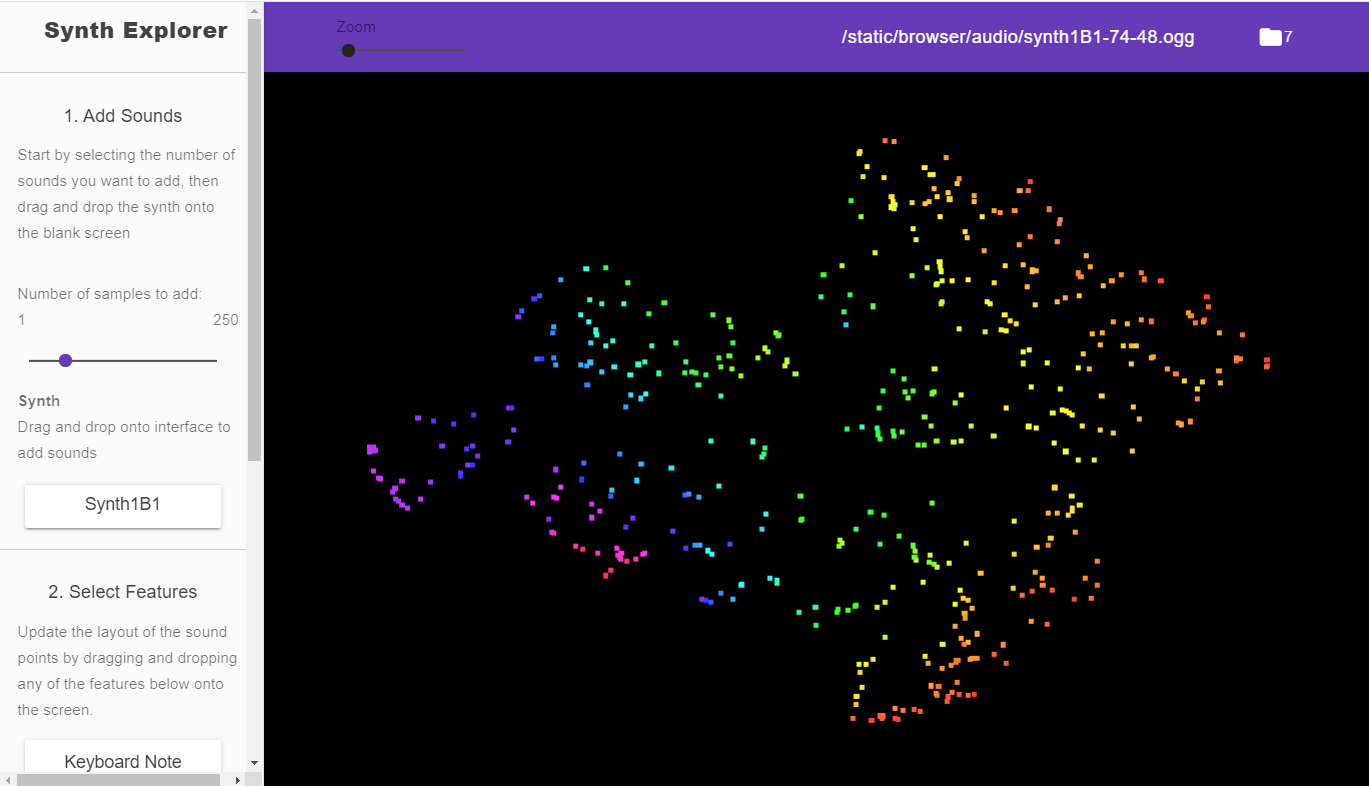
\includegraphics[width=0.8\textwidth]{SynthExplore Init.png}
    \caption{Synth Explorer User Interface}
    \label{fig:ui_1}
\end{figure}

\subsubsection{Adding Sounds}
The space of possible sounds that can be produced by a synthesizer is vast. Ten thousand four second audio clips of patches from \textit{torchsynth} represents only a subset of the possible sounds that torchsynth is capable of producing. That being said, presenting a user with ten thousand audio clips on a 2D layout would also be overwhelming. The user is initially presented with a small random subset of possible outcomes. The user is given the option to control how many sounds are added to the visualization at once using a slider control that ranges between 1 and 250. They are then able to add that many sounds to the their visualization by dragging and dropping the UI object representing a particular synthesizer onto the visualization area. In this way they can explore the sound space in an iterative fashion. This section of the user interface is shown in figure \ref{fig:steup 1}. Currently only one synthesizer is shown in the interface, however any number could be included. This would allow the user to compare and explore multiple synthesizers at any given time. 

Once a user drops a synthesizer onto the visualization, the requested number of synthesizer sounds are randomly selected from the database and added to the interface. A single sound is represented as a single point on the 2D visualization.

\begin{figure}
    \centering
    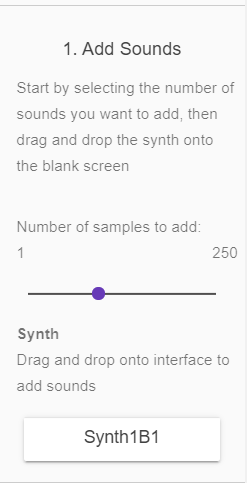
\includegraphics[width=0.2\linewidth]{SynthExplore_AddSounds.png}
    \caption{Synth Explorer Step 1}
    \label{fig:steup 1}
\end{figure}

\subsubsection{Constructing the visualization}
The next section of the user interface is focused on allowing the user to control their visualization. Specifically, this section allows users to decide which features are assigned to which dimension of the visualization. The available features are shown on the left side of user interface in figure \ref{fig:features}. Using the same drag and drop paradigm, the user is able to drag any of the features onto the visualization surface in order to modify the layout of audio samples. When the user initiates a drag and drop interaction, large drop areas representing the different dimensions of the visualization appear for the user to choose from. The available dimensions are the x-axis, y-axis, and the color of the points. Once a feature is dropped onto one of the dimensions of the visualization, the points representing the sounds automatically shift into the new position to reflect the changes. Any feature can be associated with any dimension, allowing the user to explore the relationship between the features and develop a visualization that meets their needs.

A decision was made to use the technical names of the features. While this may be confusing to some users, there are unfortunately not many great alternatives to this problem. Tooltips are provided to give novices an approximate non-technical description of the feature -- the hope is that these users will still feel inspired to explore these different features and learn how they relate to the auditory dimensions of sounds.

\begin{figure*}
    \centering
    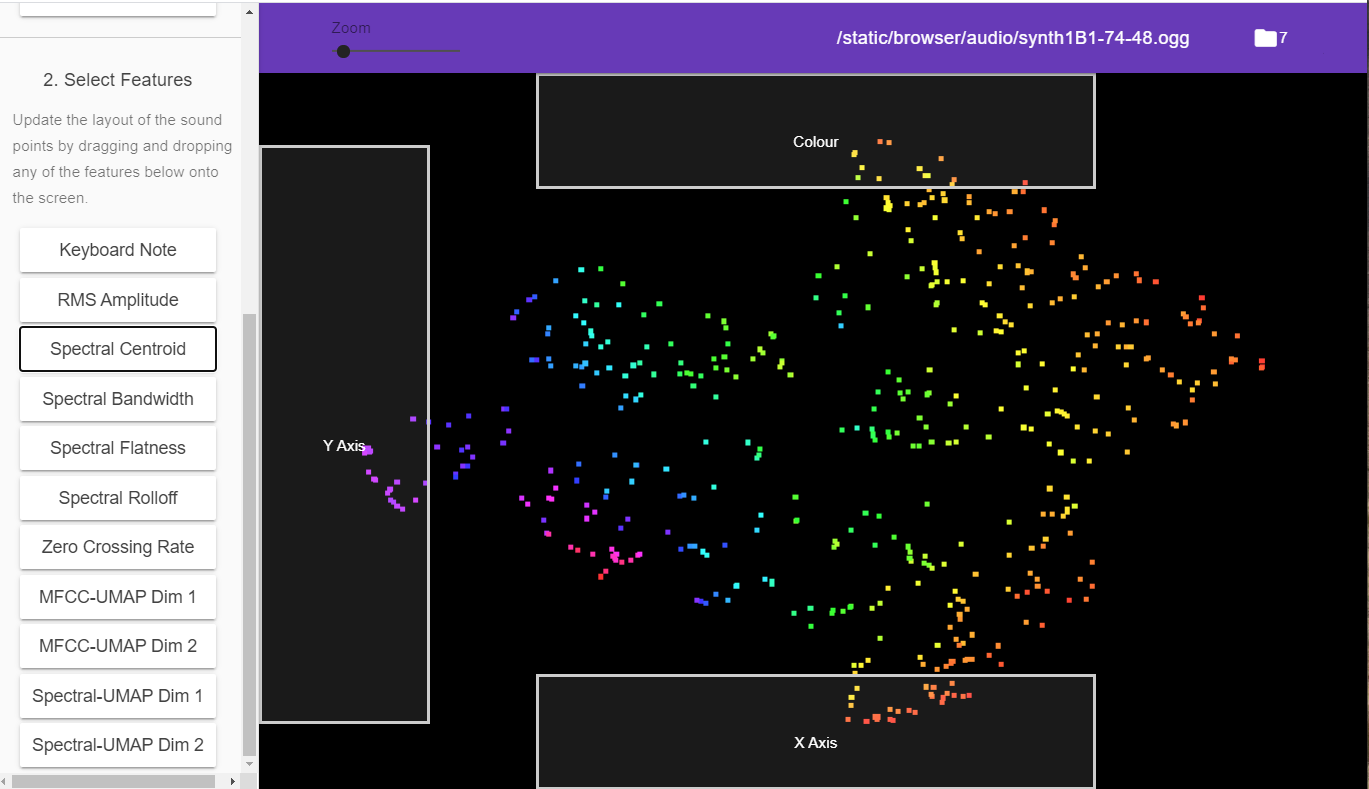
\includegraphics[width=0.9\textwidth]{SynthExplore A.png}
    \caption{Synth Explorer UI: Updating features}
    \label{fig:features}
\end{figure*}


\subsubsection{Exploring and Saving Sounds}
The majority of the space on the user interface is occupied by the 2D browsing space, which is shown in figure 2. This is the space where synthesizer sounds are represented as points on a scatter plot. To listen to a particular sound, the user simply needs to hover their cursor over the point representing a sound. They receive both auditory and visual feedback once they intersect with a point. The sound represented by the point plays and a small circle burst the same color as the point is animated into view at the point of interaction. Users can also zoom into the visualization using their mouse scroll wheel and navigate the space using a click and drag operation. Each of these gestures is meant to reflect operations that would feel intuitive and natural to an experienced computer user.

This mode of interaction provides a fast way for the user to preview a large number of samples. The goal of the 2D layout and exploration method is to provide the user with an embodied method for exploring sounds. The 2D spatial layout using colors provides users with a visual representation of the sonic space that they can interact with and create their own associations with. The interaction itself is easy to master as it simply requires dragging a mouse around the screen and listening to sounds. Modifying the layout using drag and drop interactions also requires little conscious effort. These intuitive interactions were implemented to support situated creativity and thereby aid creative flow.

When a user has listened to a sound that they like and want to save, they can press the 's' key on their keyboard to save that clip to a 'sound palette'. This is equivalent to adding an item to an online shopping cart. The user can then continue to explore sounds.

At this point the user is able repeat any of the preceding steps and continue explore the visualization: add more sounds, modify the dimensions with different features, explore the space, adjust parameters for a specific sound, and then save the resulting sounds.

\subsubsection{Adjusting Parameters}
At any point during exploration users can move to a secondary interface and work directly with the synthesizer parameters. This interface, shown in figure \ref{fig:adjusting-parameters}, is essentially a regular control interface for the torchsynth synthesizer that contains slider controls to update the values for all 78 of the parameters in the torchsynth Voice. These 78 parameters are grouped by the specific module that they control (see \ref{fig:voice_diagram} for a diagram of all the modules in Voice). When navigating to this screen, the parameter settings for the sound that was selected from the visual exploration interface will be showing, this allows the user to gain insight into the specific parameter values for that particular sound, as well as to make modifications on the sound.

\begin{figure}[ht]
    \centering
    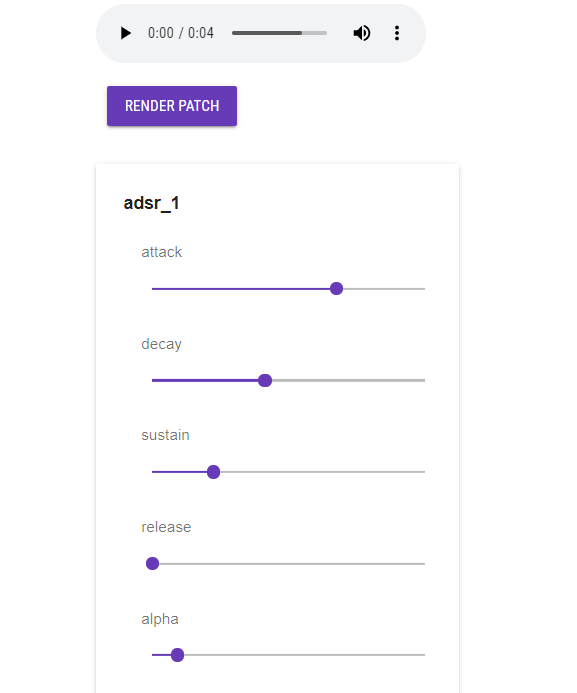
\includegraphics[width=0.45\textwidth]{figures/synthexplore/SynthExplore-Adjust-Param-Cropped.png}
    \caption{Interface for adjusting the parameter values for a synthesizer patch, allowing for fine-tuning of sounds found on the visual exploration interface }
    \label{fig:adjusting-parameters}
\end{figure}

\subsubsection{Downloading}
Once the user has sufficiently explored the sonic space and saved a palette of sounds they would like to use, they can click on the download icon next to their saved sounds and download all the synthesizer sound files they saved. Once they have done this they are free to use those sounds for whatever creative task they would like.

\subsection{Technical Implementation Details}
Synth Explorer is implemented as a web application. The Django framework\footnote{\url{https://www.djangoproject.com/}} was used to implement the backend of the web app. Django is written in python and provides an elegant data-model system for interacting with a database such as MySQL\footnote{{https://www.mysql.com/}}. The sound generation and analysis portion of the application is written as a Django management command -- when this command is run, a set of sounds is rendered using \textit{torchsynth}, and analyzed using librosa and UMAP. Once the samples have been analyzed and audio files saved to disk, the audio features and patch settings for each sound is saved in a MySQL database.

The frontend of the application is written using HTML, CSS, and JavaScript. The foundation of the application was based on code developed by Leon Feddden \footnote{\url{https://github.com/fedden/umap_tsne_embedding_visualiser}}. This code was modified to function within the Django framework and the user interaction paradigm was modified to support dynamic adding of synthesizer samples and user construction of the layout using drag and drop interactions. The visualization and animation is rendered using three.js\footnote{\url{https://threejs.org/}}.

\section{Evaluation}
\subsection{Creativity Support Index}
The creativity support index (CSI) \cite{cherry2014quantifying} is a psychometric survey that was designed to quantify the ability of a tool to assist a user with a creative task. The CSI evaluates a creativity support tool based on six different criteria: Exploration, Expressiveness, Immersion, Enjoyment, Results Worth Effort, and Collaboration. The CSI is structured as a questionnaire with two different sections. The first sections contains 12 questions, shown in figure \ref{fig:csi}, which participants answer with a score from 1-10 ("Highly Disagree" to "Highly Agree"). The second section contains 15 questions which compares each of the evaluation criteria pairwise and asks the participant the evaluate which criteria was better supported; for example, each question begins with “When doing this task, it’s most important that I’m able to...” followed by a two statements, where one statement is related to one of the evaluation criteria and the other is related to another. Participants are asked to select only of the statements and each evaluation criteria is ranked against all the others. Based on the scores for these questions a CST is given a score out of 100. Synth Explorer was evaluated informally on two separate tasks that were designed to replicate a typical synthesizer use case in the context of music production.

\begin{figure}[ht]
    \centering
    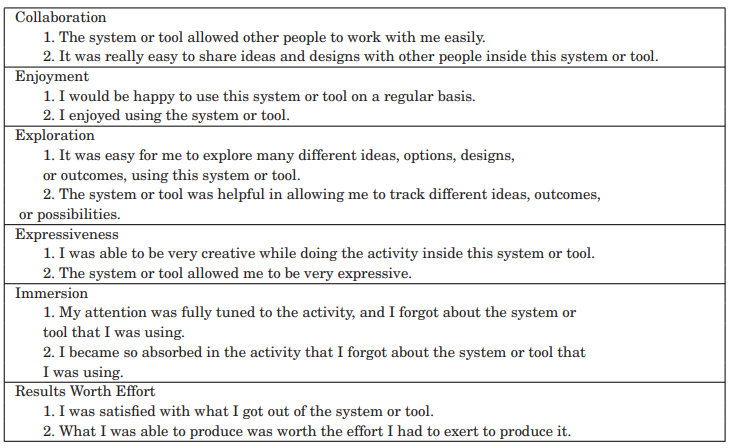
\includegraphics[width=0.99\textwidth]{figures/synthexplore/CSI-Questions.png}
    \caption{Agreement questions for the creativity support index}
    \label{fig:csi}
\end{figure}

\subsubsection{Task 1: Synthesizer browsing for an existing project}
In this task the user is working on an existing musical project in a separate workstation. They are composing a piece of music and then are asked to find a new synthesizer sound for an additional track to their composition. They must leave the workstation,
open Synth Explorer, browse for a new sound, then leave Synth Explorer and open the new sound back in the workstation they were initially working within.

\subsubsection{Task 2: Creating a sound palette for a new project}
In this task the user is beginning a new project and is searching for a set of synthesizer sounds to create the sonic palette for the new composition. They may have a particular sound in mind, but are asked to explore the interface in an open-minded way to look for new sounds and create a collection as inspiration to start the new project.

\subsection{CSI Results}
Results of the CSI evaluation are shown in table \ref{table:csi}. These results show that Synth Explorer supported task 1 to a greater degree than task 2. Task 1 received an overall score of 78.67 whereas task 2 received an overall score of 71.67. The results showed that collaboration was not supported and received a score of zero for both tasks. This makes sense considering the nature of the tasks and the tool itself. Collaboration was not a part of the evaluated tasks, however, the tool itself does not currently support collaboration in any meaningful way other than allowing two users to sit next to each other and browse for synth sounds simultaneously. The tool supported exploration in both tasks more than any of the other attributes evaluated. This result is positive considering that was one of the major goals for the tool. Another area that was well supported by the tool is enjoyment, while the results and expressiveness of the tool itself were not highly rated. The lack of expressiveness also makes sense for the tool; Synth Explorer itself does not necessarily allow expression -- it allows a user to explore sounds with the goal of maintaining a creative flow in a large creative context, but it is more challenging to actually be expressive with the tool.

The results section of the evaluation did not score highly either. This was due to the fact that the 2D layout of sounds was still challenging to navigate and make sense of. This is in part due to the underlying method for generating sounds as well as the sound mapping techniques. Randomly sampling a synthesizer is not the best way to capture meaningful sounds from the synthesizer and a lot of times produces dramatic or unusable results. This lead to a large portion of the sounds being a bit too wild for the tasks at hand. Additionally, capturing sound similarity in two dimensions is still an open question that requires further work. Despite this, the interface was effective at enabling rapid exploration of a large number of sounds and it was enjoyable getting to explore manipulating the visualization by dragging and dropping the different features onto the plot.

\begin{table}[th]
\centering
\begin{tabular}{l|llll|ll}
Area           & Q1 & Q2 & T1 & T2 & T1 Total   & T2 Total \\
\hline
Collaboration  & 1  & 1  & 0            & 0            & 0              & 0            \\
Enjoyment      & 7  & 8  & 5            & 4            & 75             & 60           \\
Exploration    & 10 & 7  & 5            & 5            & 85             & 85           \\
Expressiveness & 5  & 4  & 1            & 2            & 9              & 18           \\
Immersion      & 8  & 7  & 3            & 2            & 45             & 30           \\
Results        & 5  & 6  & 2            & 2            & 22             & 22           \\
Total Score    &    &    &              &              & \textbf{78.67} & \textbf{71.67} 
\end{tabular}
\caption{Results of creativity support index questionnaire.}
\label{table:csi}
\end{table}

\section{Future Work and Conclusion}
This chapter has introduced the Synth Explorer creativity support tool. The intention of this tool is to support users in the process of working with synthesizers and finding new sounds for creative projects. The development of Synth Explorer was based on a set of design principles informed by the fields music interaction and creativity support tools. A further goal of the tool is to support novice users who might have experience in music production, but do not have experience working with synthesizers. Synth Explorer was designed to support novices using an approach to creativity support based on cognitive theory which emphasizes embodied, situated, and distributed creativity. The designed tool uses a 2D visualization of synthesizer sounds to arrange sounds spatially as well as uses colors to support an embodied approach to exploration. By using a simple drag and drop interface and quick browsing of sounds using a visual layout, users are able to quickly start exploring and remain engage in their creative task. A secondary interface containing the individual parameter values allows users to engage in manual synthesizer programming using a sound from the visual interface as a starting point. This encourages long-term engagement through the inclusion of a more challenging interaction paradigm that provides a user with more depth of control.

An evaluation of the tool using the creativity support index revealed insight into the strengths and weaknesses of the tool and helped to identify some areas for potential further work. The most glaring limitation of the tool is it's lack of support for collaboration. The current version of the system has no support for collaboration, however this could be added relatively easily based on the implementation. Since Synth Explorer is built as a web application using the Django framework, a user login system could be added quite easily which would allow users to save and share collections of sounds that they have curated. Different synthesizers and layouts could also be shared through a system like this. Another limitation of the current system is in the available options to filter and search for sounds. Currently the user is limited to added random samples to the interface and exploring different configurations of that. In order to support users in arriving at more useful results and collections of sounds, providing additional search options such as a search by similarity or providing additional tools for selecting and filtering the current selection would be a good area for future work as well. Integrating more advanced sound searching methods such as an example-based interaction paradigm using one of the approaches discussed in \S\ref{chapter:inverse_synth_experiment} would also provide a good area for future development. 
	\chapter{Future Work and Conclusion}

\section{Future Work}
\cite{ramirez2021differentiable} -- including VSTis in the training loop and calculating the loss directly on an audio representation.

\section{Conclusion}
	\appendix
	\startappendix{Model Architectures}
\label{appendix:spiegelib_models}

The model architectures provided below were used in the experiments conducted in chapter \ref{chapter:inverse_synth_experiment}. Each model estimated a subset of nine parameters from $Dexed$ to match a target audio. $n$ is the batch size:

\begin{table}[ht]
\caption{MFCC MLP}
\centering
\begin{tabular}{l|l|l}
Layer Type & Output Shape & Num Parameters \\ \hline
Input & (n, x) & \\
Dense & (n, 256) & 146688\\
ReLU    & (n, 256) &\\
Dense & (n, 128) & 32896\\
ReLU    & (n, 128) &  \\
Dense & (n, 64) & 8256 \\
ReLU    & (n, 64) & \\
Dropout (0.3) & (n, 64) & \\
Dense   & (n, 7) & 455\\
\hline
\hline
Total   & \ & 188,295\\
\end{tabular}
\end{table}

\begin{table}[ht]
\caption{Mel-Spectrogram MLP}
\centering
\begin{tabular}{l|l|l}
Layer Type & Output Shape & Num Parameters \\ \hline
Input & (n, x) & \\
Dense & (n, 256) & 721152\\
ReLU    & (n, 256) &\\
Dense & (n, 128) & 32896\\
ReLU    & (n, 128) &  \\
Dense & (n, 64) & 8256 \\
ReLU    & (n, 64) & \\
Dropout (0.4) & (n, 64) & \\
Dense   & (n, 7) & 455\\
\hline
\hline
Total   & \ & 762,759\\
\end{tabular}
\end{table}

\begin{table}[ht]
\caption{MFCC LSTM}
\centering
\begin{tabular}{l|l|l}
Layer Type & Output Shape & Num Parameters \\ \hline
Input & (n, x) & \\
LSTM & (n, 44, 64) & 19968\\
LSTM & (n, 44, 64) & 33024\\
LSTM & (n, 64) & 33024\\
Dropout (0.3) & (n, 64) & \\
Dense   & (n, 7) & 455\\
\hline
\hline
Total   & \ & 86,471\\
\end{tabular}
\end{table}

\begin{table}[ht]
\caption{Mel-Spectrogram LSTM}
\centering
\begin{tabular}{l|l|l}
Layer Type & Output Shape & Num Parameters \\ \hline
Input & (n, x) & \\
LSTM & (n, 64, 128) & 88576\\
LSTM & (n, 64, 128) & 131584\\
LSTM & (n, 128) & 131584\\
Dropout (0.2) & (n, 128) & \\
Dense   & (n, 7) & 903\\
\hline
\hline
Total   & \ & 352,647\\
\end{tabular}
\end{table}

\begin{table}[ht]
\caption{MFCC LSTM++}
\centering
\begin{tabular}{l|l|l}
Layer Type & Output Shape & Num Parameters \\ \hline
Input & (n, x) & \\
Bidirectional LSTM & (n, 256) & 145408\\
Dropout (0.3) & (n, 256) & \\
Dense & (n, 128) & 32896\\
ELU & (n, 128) &\\
Highway Layer 1-7 & (n, 128) & 33024\\
Dense   & (n, 7) & 903\\
\hline
\hline
Total   & \ & 410,375\\
\end{tabular}
\end{table}

\begin{table}[ht]
\caption{Mel-Spectrogram LSTM++}
\centering
\begin{tabular}{l|l|l}
Layer Type & Output Shape & Num Parameters \\ \hline
Input & (n, x) & \\
Bidirectional LSTM & (n, 256) & 177152\\
Dropout (0.4) & (n, 256) & \\
Dense & (n, 128) & 32896\\
ELU & (n, 128) &\\
Highway Layer 1-7 & (n, 128) & 33024\\
Dense   & (n, 7) & 903\\
\hline
\hline
Total   & \ & 442,119\\
\end{tabular}
\end{table}

\begin{table}[ht]
\caption{MFCC CNN}
\centering
\begin{tabular}{l|l|l|l}
Layer Type & Kernel Size & Output Shape & Num Parameters \\ \hline
Input & \ & (n, x) & \\
Conv2D (Stride=2,2) & (3,3) & (n, 22, 7, 16) & 160\\
ReLU                &       & (n, 22, 7, 16) & \\
Batch Normalization &       & (n, 22, 7, 16) & 64 \\
Conv2D (Stride=2,2) & (3,3) & (n, 11, 4, 32) & 4640\\
ReLU                &       & (n, 11, 4, 32) & \\
Batch Normalization &       & (n, 22, 7, 16) & 128 \\
Conv2D (Stride=2,2) & (3,3) & (n, 6, 2, 32) & 9248\\
ReLU                &       & (n, 6, 2, 32) & \\
Batch Normalization &       & (n, 22, 7, 16) & 128 \\
Conv2D (Stride=2,2) & (3,3) & (n, 3, 1, 64) & 18496\\
ReLU                &       & (n, 3, 1, 64) & \\
Batch Normalization &       & (n, 22, 7, 16) & 256 \\
Conv2D (Stride=2,2) & (3,3) & (n, 2, 1, 64) & 36928\\
ReLU                &       & (n, 2, 1, 64) & \\
Batch Normalization &       & (n, 22, 7, 16) & 256 \\
Dropout (0.3)       &       & (n, 2, 1, 64) & \\
Flatten             &       & (n, 128) & \\
Dense 				& 		& (n, 512) & 66048\\
Dropout (0.3) 		& 		& (n, 512)  & \\
Dense 				& 		& (n, 512) & 262656\\
Dropout (0.3) 		& 		& (n, 512)  & \\
Dense               &       & (n, 7) & 3591\\
\hline
\hline
Total               &       &        & 402,599\\
\end{tabular}
\end{table}

\begin{table}[ht]
\caption{Mel-Spectrogram CNN}
\centering
\begin{tabular}{l|l|l|l}
Layer Type & Kernel Size & Output Shape & Num Parameters \\ \hline
Input & \ & (n, x) & \\
Conv2D (Stride=2,2) & (3,3) & (n, 32, 22, 16) & 160\\
ReLU                &       & (n, 32, 22, 16) & \\
Conv2D (Stride=2,2) & (3,3) & (n, 16, 11, 32) & 4640\\
ReLU                &       & (n, 16, 11, 32) & \\
Conv2D (Stride=2,2) & (3,3) & (n, 8, 6, 32) & 9248\\
ReLU                &       & (n, 8, 6, 32) & \\
Conv2D (Stride=2,2) & (3,3) & (n, 4, 3, 64) & 18496\\
ReLU                &       & (n, 4, 3, 64) & \\
Conv2D (Stride=2,2) & (3,3) & (n, 2, 2, 64) & 36928\\
ReLU                &       & (n, 2, 2, 64) & \\
Dropout (0.3)       &       & (n, 2, 2, 64) & \\
Flatten             &       & (n, 256) & \\
Dense 				& 		& (n, 128) & 32896\\
Dropout (0.3) 		& 		& (n, 128)  & \\
Dense 				& 		& (n, 128) & 16512\\
Dropout (0.3) 		& 		& (n, 128)  & \\
Dense 				& 		& (n, 128) & 16512\\
Dropout (0.3) 		& 		& (n, 128)  & \\
Dense               &       & (n, 7) & 903\\
\hline
\hline
Total               &       &        & 136,295\\
\end{tabular}
\end{table}

	\startappendix{GAN Architecture Details}

In Tables \ref{wavegan_gen} and \ref{wavegan_gen_resize} we present our architectures for the Transpose Convolution and Resize-based 1-dimensional generators. In Table \ref{wavegan_disc} we present our architecture for the 1-dimensional discriminator. In Tables \ref{melgan_gen} and \ref{melgan_disc} we present the architectures for the MelGAN generator and discriminator. In Table \ref{param_table} we present parameters relevant to both GANs.

Layers with a (*) refer to `optional' layers which we experimented with keeping or removing. The batch size is referred to as $n$ and $k$ is the kernel size, which is either 5, 15, or 25.

\begin{table}[H]
\caption{Transpose Convolution Waveform Generator}\label{wavegan_gen}
\centering
\begin{tabular}{l|l|l}
Operation & Kernel Size & Output Shape \\ \hline
Input $\sim$ Uniform(-1,1) & \  & (n,100)\\
Dense 1 & (100,16384) & (n,16384)\\
Reshape & \ & (n,16,1024)\\
Leaky ReLU & \ & (n,16,1024)\\
(*) Dropout (50\%) & \ & (n,16,1024)\\
Trans Conv1D (Stride=4) & (25,1024,512) & (n,64,512)\\
Leaky ReLU & \  & (n,64,512)\\
(*) Dropout (50\%) & \  & (n,64,512)\\
Trans Conv1D (Stride=4) & (25,512,256) & (n,256,256)\\
Leaky ReLU & \  & (n,256,256)\\
(*) Dropout (50\%) & \  & (n,256,256)\\
Trans Conv1D (Stride=4) & (25,256,128) & (n,1024,128)\\
Leaky ReLU & \  & (n,1024,128)\\
(*) Dropout (50\%) & \  & (n,1024,128)\\
Trans Conv1D (Stride=4) & (25,128,64) & (n,4096,64)\\
Leaky ReLU & \  & (n,4096,64)\\
(*) Dropout (50\%) & \  & (n,4096,64)\\
Trans Conv1D (Stride=4) & (25,64,1) & (n,16384,1)\\
Tanh & \  & (n,16384,1)\\
\end{tabular}
\end{table}

\begin{table}
\caption{Resize Convolution Waveform Generator}\label{wavegan_gen_resize}
\centering
\begin{tabular}{l|l|l}
Operation & Kernel Size & Output Shape \\ \hline
Input $\sim$ Uniform(-1,1) & \  & (n,100)\\
Dense 1 & (100,16384) & (n,16384)\\
Reshape & \ & (n,16,1024)\\
Leaky ReLU & \ & (n,16,1024)\\
(*) Dropout (50\%) & \ & (n,16,1024)\\
Resize (Factor=4) & \ & (n,64,1024)\\
Conv1D (Stride=1) & (25,1024,512) & (n,64,512)\\
Leaky ReLU & \  & (n,64,512)\\
(*) Dropout (50\%) & \  & (n,64,512)\\
Resize (Factor=4) & \ & (n,256,512)\\
Conv1D (Stride=1) & (25,512,256) & (n,256,256)\\
Leaky ReLU & \  & (n,256,256)\\
(*) Dropout (50\%) & \  & (n,256,256)\\
Resize (Factor=4) & \ & (n,1024,256)\\
Conv1D (Stride=1) & (25,256,128) & (n,1024,128)\\
Leaky ReLU & \  & (n,1024,128)\\
(*) Dropout (50\%) & \  & (n,1024,128)\\
Resize (Factor=4) & \ & (n,4096,128)\\
Conv1D (Stride=1) & (25,128,64) & (n,4096,64)\\
Leaky ReLU & \  & (n,4096,64)\\
(*) Dropout (50\%) & \  & (n,4096,64)\\
Resize (Factor=4) & \ & (n,16384,64)\\
Conv1D (Stride=1) & (25,64,1) & (n,16384,1)\\
Tanh & \  & (n,16384,1)\\
\end{tabular}
\end{table}

\begin{table}[H]
\caption{Waveform Discriminator}\label{wavegan_disc}
\centering
\begin{tabular}{l|l|l}
Operation & Kernel Size & Output Shape \\ \hline
Input $\boldsymbol{x}$ or $G(\boldsymbol z)$ & \  & (n,16384,1)\\
Conv1D (Stride=4) & (k,1,64) & (n,4096,64)\\
Leaky ReLU & \ & (n,4096,64) \\
Dropout (30\%) & \ & (n,4096,64)\\
(*) Phase Shuffle ($N$=2) & \ & (n,4096,64)\\
Conv1D (Stride=4) & (k,64,128) & (n,1024,128)\\
Leaky ReLU & \ & (n,1024,128) \\
Dropout (30\%) & \ & (n,1024,128)\\
(*) Phase Shuffle ($N$=2) & \ & (n,1024,128)\\
Conv1D (Stride=4) & (k,128,256) & (n,256,256)\\
Leaky ReLU & \ & (n,256,256) \\
Dropout (30\%) & \ & (n,256,256)\\
(*) Phase Shuffle ($N$=2) & \ & (n,256,256)\\
Conv1D (Stride=4) & (k,256,512) & (n,64,512)\\
Leaky ReLU & \ & (n,64,512) \\
Dropout (30\%) & \ & (n,64,512)\\
(*) Phase Shuffle ($N$=2) & \ & (n,64,512)\\
Conv1D (Stride=4) & (k,512,1024) & (n,16,1024)\\
Leaky ReLU & \ & (n,16,1024) \\
Dropout (30\%) & \ & (n,16,1024)\\
(*) Phase Shuffle ($N$=2) & \ & (n,16,1024)\\
Reshape &\ & (n,16384)\\
Dense &\ (16384,1) & (n,1)
\end{tabular}
\end{table}





\begin{table}[H]
\caption{Resize Convolution MelGAN Generator}\label{melgan_gen}
\centering
\begin{tabular}{l|l|l}
Operation & Kernel Size & Output Shape \\ \hline
Input $\sim$ Uniform(-1,1) & \  & (n,100)\\
Dense 1 & (100,16384) & (n,16384)\\
Reshape & \ & (n,4,4,1024)\\
Leaky ReLU & \ & (n,4,4,1024)\\
(*) Dropout (50\%) & \ & (n,4,4,1024)\\
Resize (Factor=2) & \ & (n,8,8,1024)\\
Conv2D (Stride=1) & (5,5,1024,512) & (n,8,8,512)\\
Leaky ReLU & \  & (n,8,8,512)\\
(*) Dropout (50\%) & \  & (n,8,8,512)\\
Resize (Factor=2) & \ & (n,16,16,512)\\
Conv2D (Stride=1) & (5,5,512,256) & (n,16,16,256)\\
Leaky ReLU & \  & (n,16,16,256)\\
(*) Dropout (50\%) & \  & (n,16,16,256)\\
Resize (Factor=2) & \ & (n,32,32,256)\\
Conv2D (Stride=1) & (25,25,256,128) & (n,32,32,128)\\
Leaky ReLU & \  & (n,32,32,128)\\
(*) Dropout (50\%) & \  & (n,32,32,128)\\
Resize (Factor=2) & \ & (n,64,64,128)\\
Conv2D (Stride=1) & (5,5,128,64) & (n,64,64,64)\\
Leaky ReLU & \  & (n,64,64,64)\\
(*) Dropout (50\%) & \  & (n,64,64,64)\\
Resize (Factor=2) & \ & (n,128,128,64)\\
Conv2D (Stride=1) & (5,5,64,1) & (n,128,128,1)\\
Tanh & \  & (n,128,128,1)\\
\end{tabular}
\end{table}


\begin{table}[H]
\caption{MelGAN Discriminator}\label{melgan_disc}
\centering
\begin{tabular}{l|l|l}
Operation & Kernel Size & Output Shape \\ \hline
Input $\boldsymbol{x}$ or $G(\boldsymbol z)$ & \  & (n,128,128,1)\\
Conv2D (Stride=2) & (5,5,1,64) & (n,64,64,64)\\
Leaky ReLU & \ & (n,64,64,64) \\
Dropout (30\%) & \ & (n,64,64,64)\\
(*) Phase Shuffle ($N$=2) & \ & (n,64,64,64)\\
Conv2D (Stride=2) & (5,5,64,128) & (n,1024,128)\\
Leaky ReLU & \ & (n,32,32,128) \\
Dropout (30\%) & \ & (n,32,32,128)\\
(*) Phase Shuffle ($N$=2) & \ & (n,32,32,128)\\
Conv2D (Stride=2) & (5,5,128,256) & (n,16,16,256)\\
Leaky ReLU & \ & (n,16,16,256) \\
Dropout (30\%) & \ & (n,16,16,256)\\
(*) Phase Shuffle ($N$=2) & \ & (n,16,16,256)\\
Conv2D (Stride=2) & (5,5,256,512) & (n,8,8,512)\\
Leaky ReLU & \ & (n,8,8,512) \\
Dropout (30\%) & \ & (n,64,512)\\
(*) Phase Shuffle ($N$=2) & \ & (n,64,512)\\
Conv2D (Stride=2) & (5,5,512,1024) & (n,4,4,1024)\\
Leaky ReLU & \ & (n,4,4,1024) \\
Dropout (30\%) & \ & (n,4,4,1024)\\
(*) Phase Shuffle ($N$=2) & \ & (n,4,4,1024)\\
Reshape &\ & (n,16384)\\
Dense &\ (16384,1) & (n,1)
\end{tabular}
\end{table}

\begin{table}[H]
\caption{Parameters}\label{param_table}
\centering
\begin{tabular}{l|l}
Name & Value \\ \hline
Input data type & 16-bit PCM (requantized to 32-bit float)\\
Model data type & 32-bit floating point\\
Batch size & 64, 32\\
Loss & WGAN-GP \cite{gulrajani2017improved}\\
WGAN-GP $\lambda$ & 10\\
D updates per G update & 4\\
Optimizer & Adam ($\alpha$= 1e--4, $\beta_1$= 0.9, $\beta_2$= 0.999)
\end{tabular}
\end{table}
	\graphicspath{{./}{./figures/}{./figures/neural/}}

\chapter{GAN Loss Plots}

Thoughout this section we only consider losses for the time-series based 1-dimensional GAN.
\begin{figure*}[t]
\centering
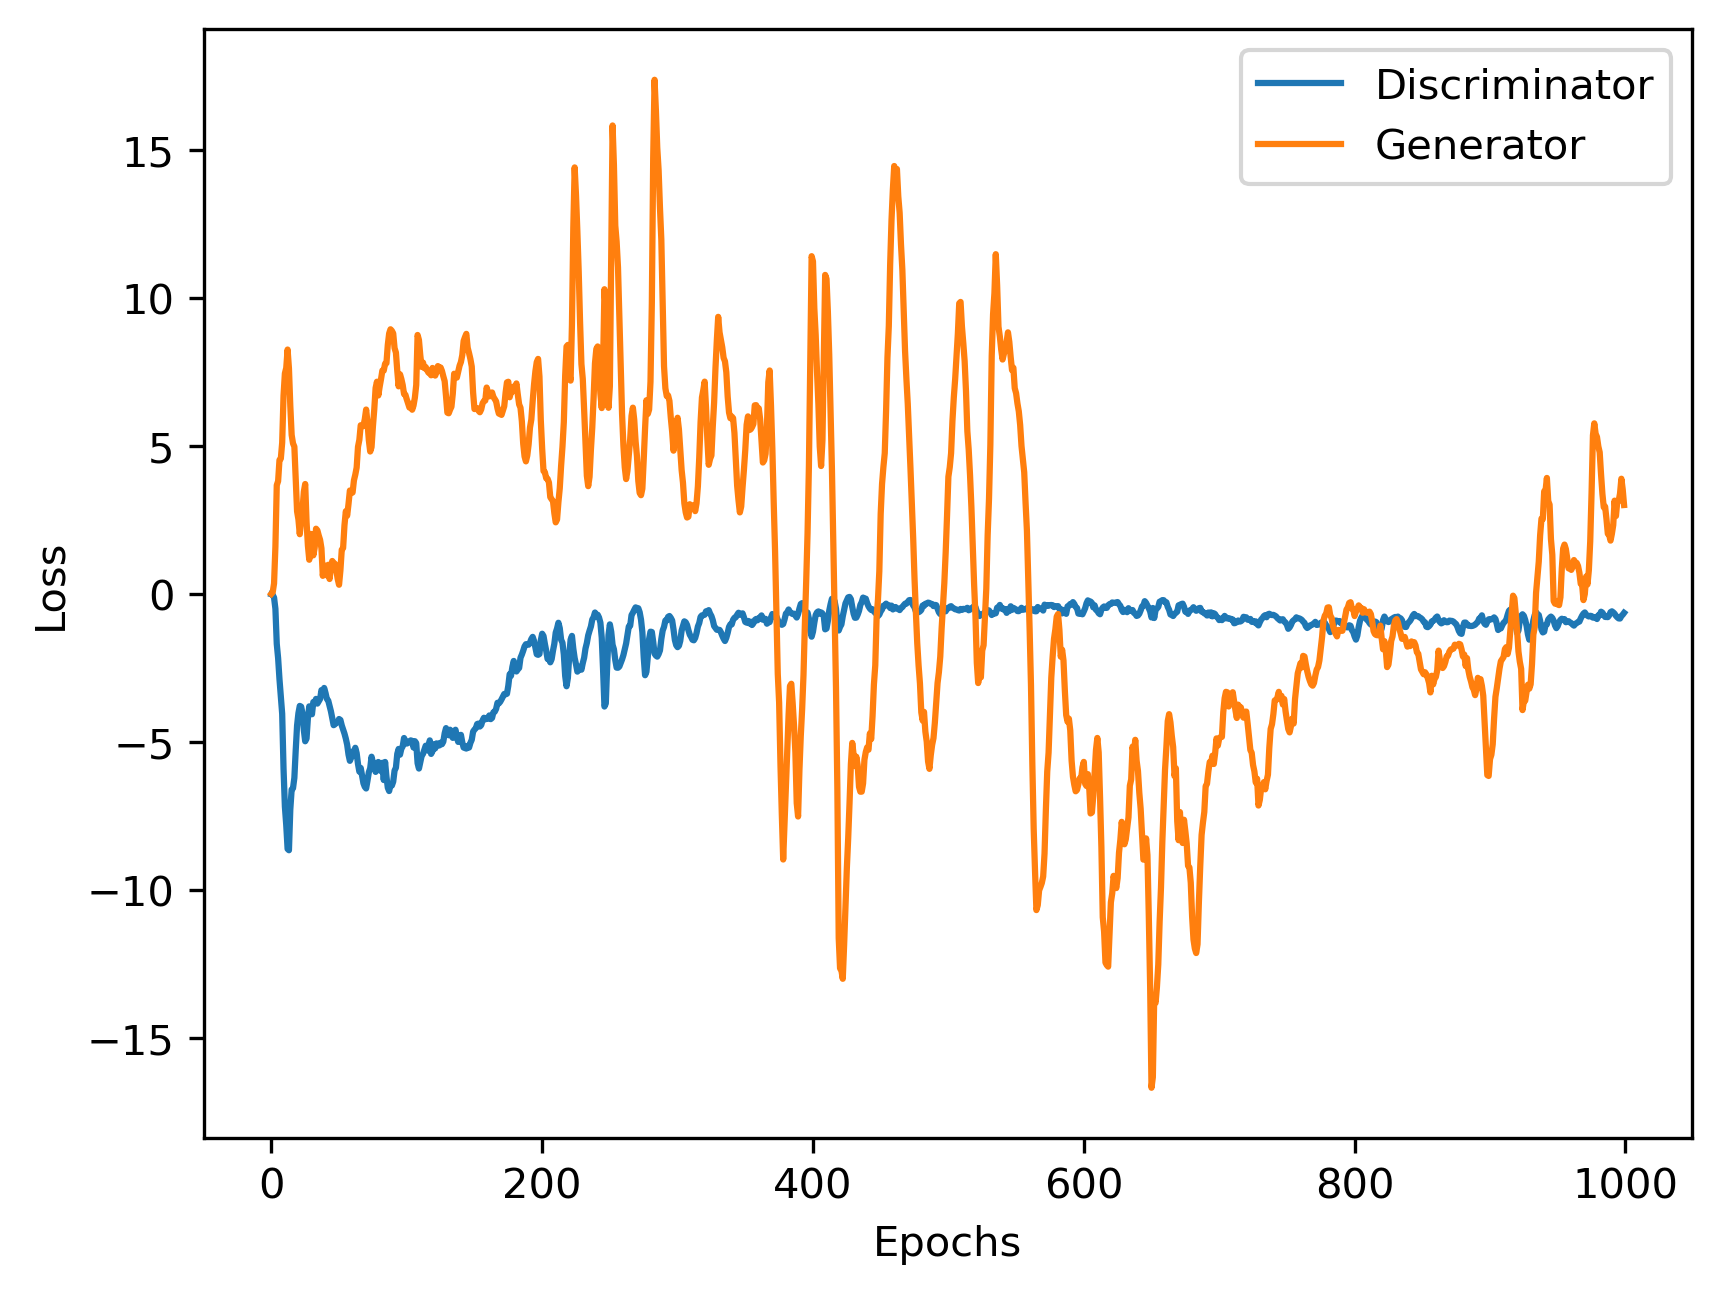
\includegraphics[width=0.45\textwidth]{loss_plots/wpgan_flute_hist_pitch_0729.png}
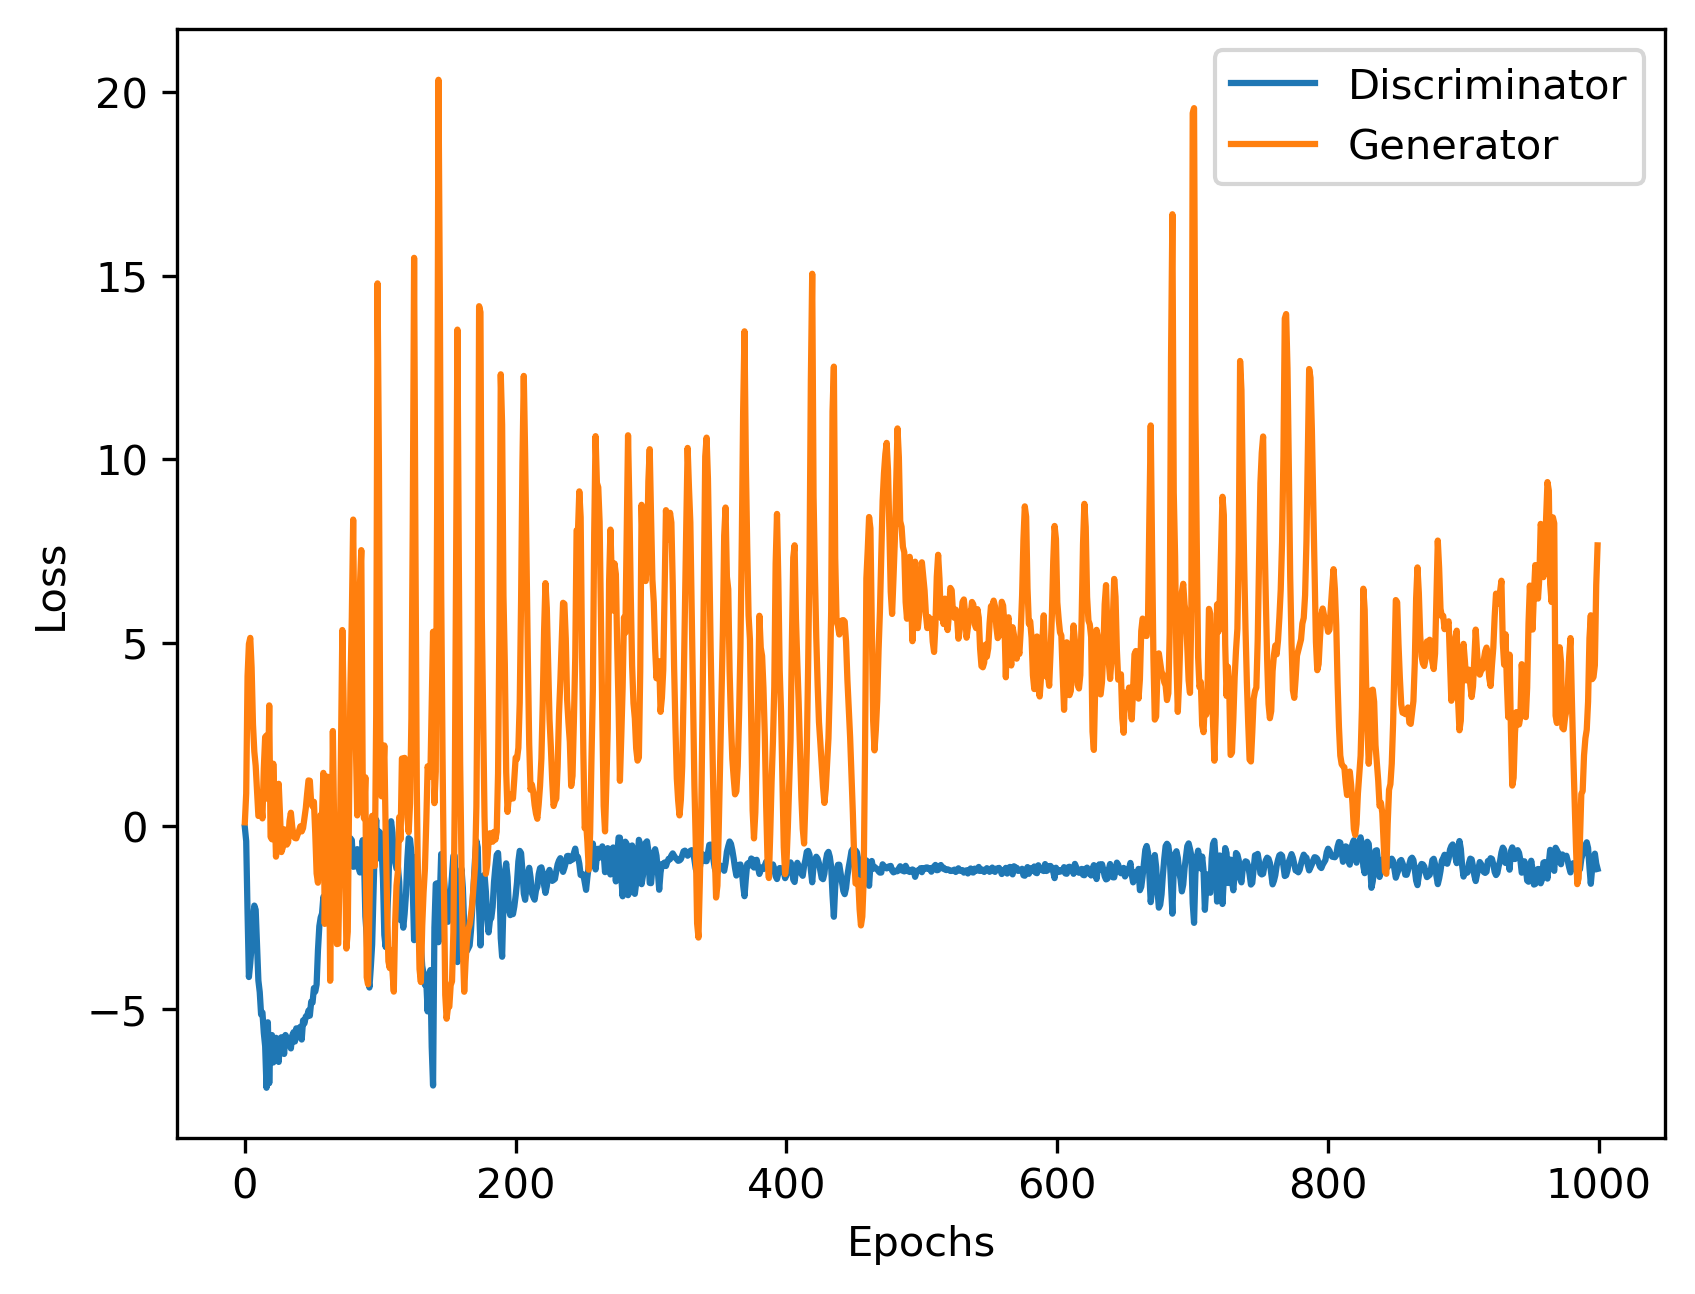
\includegraphics[width=0.45\textwidth]{loss_plots/wpgan_flute_hist_upsample_pitch_0729.png}
\caption{Left: Transpose Convolution, Right: Upsample Layer}
\end{figure*}

\begin{figure*}[t]
\centering
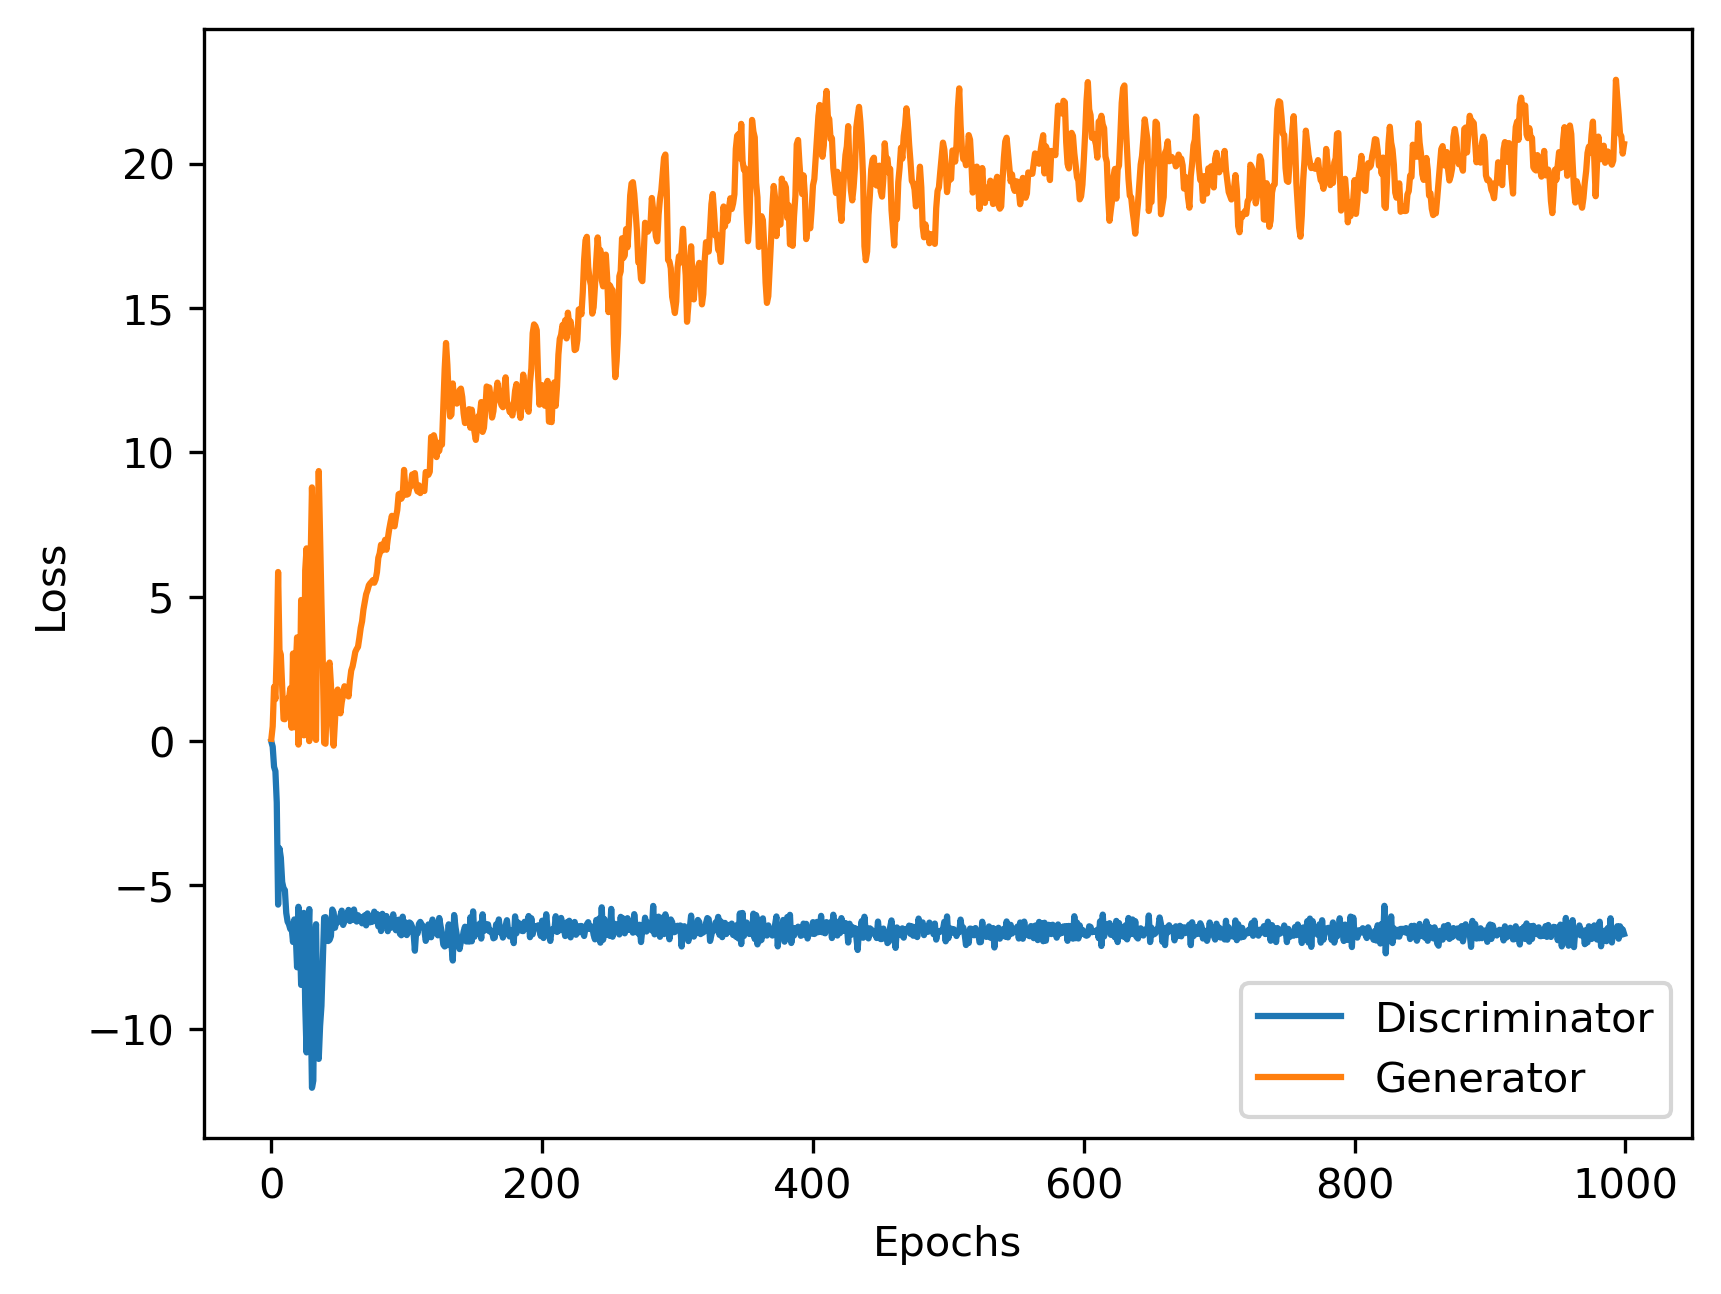
\includegraphics[width=0.45\textwidth]{loss_plots/wpgan_flute_hist_cubic_pitch_0729.png}
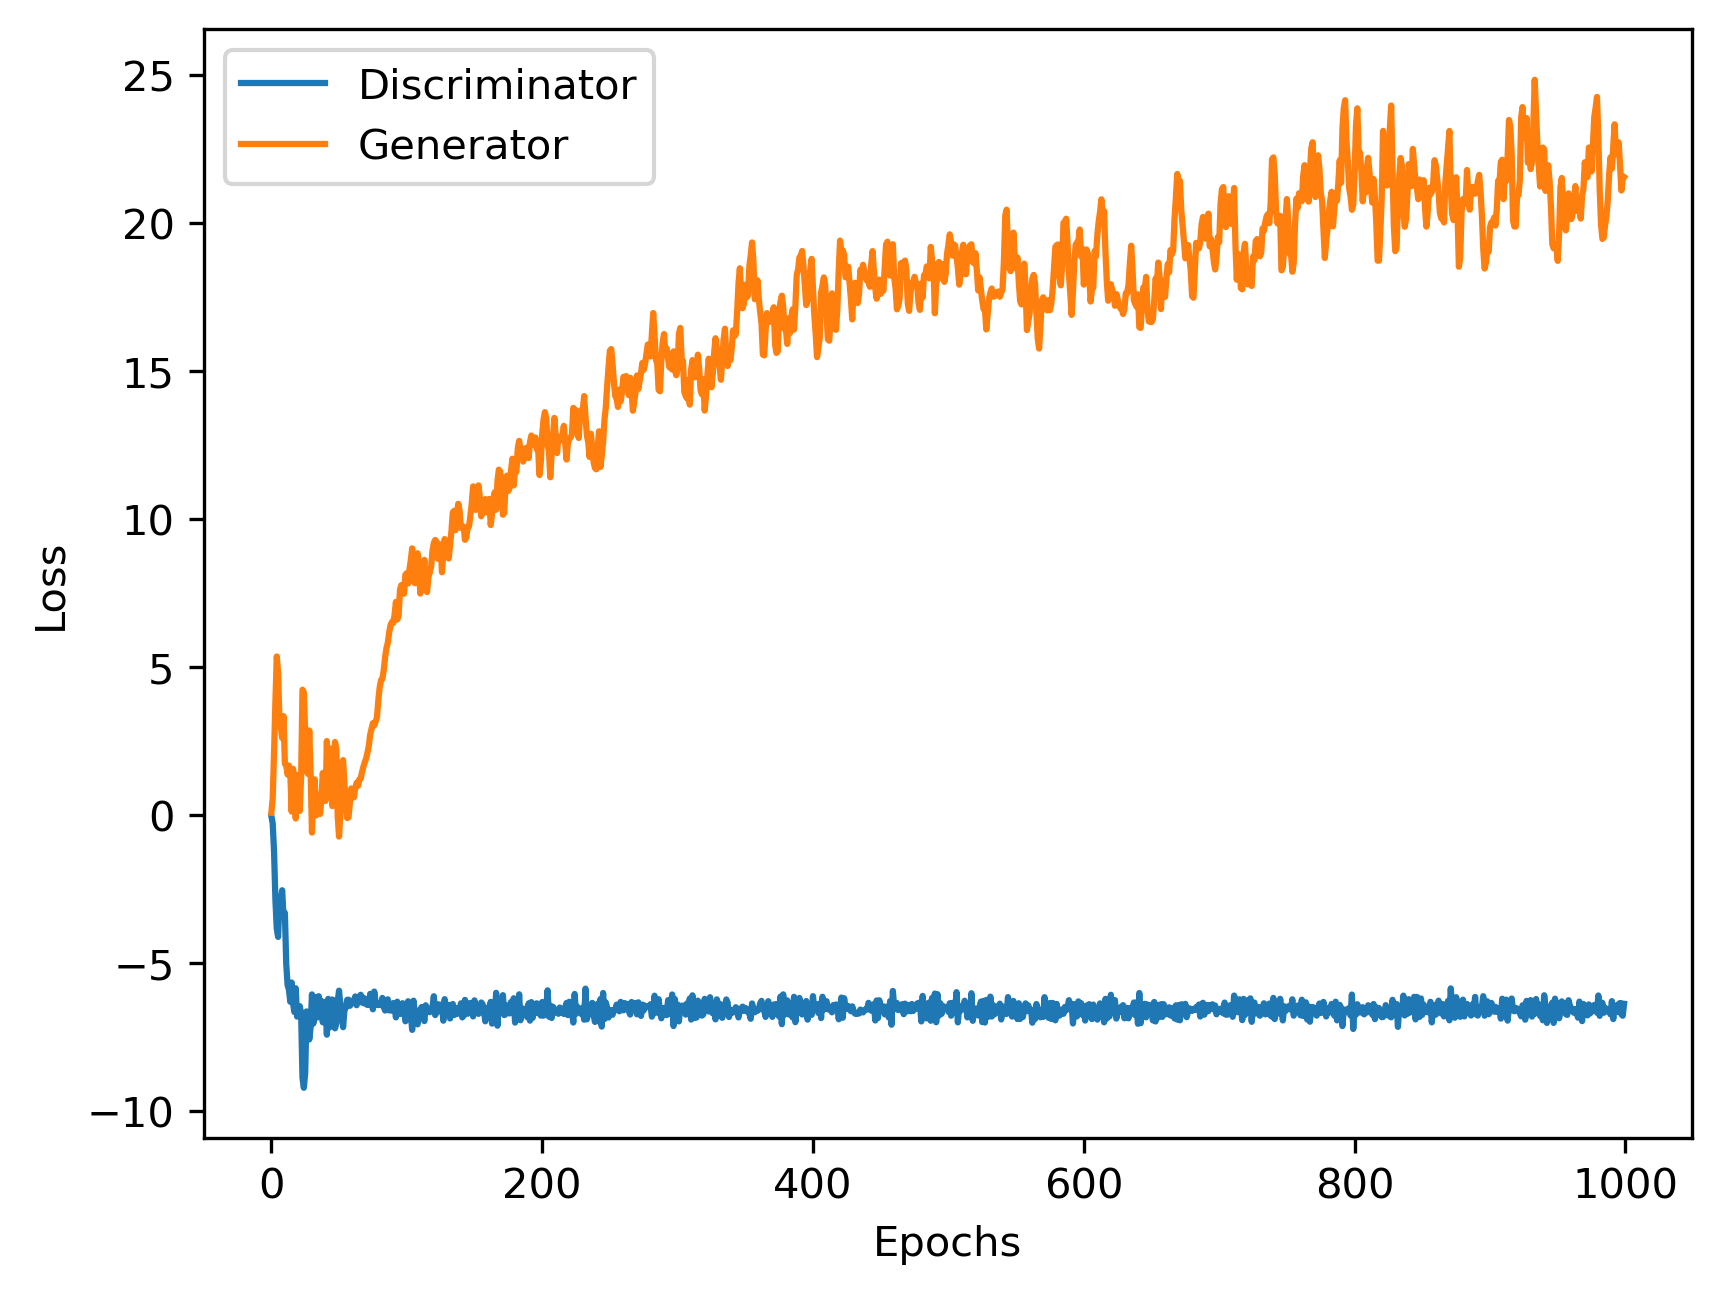
\includegraphics[width=0.45\textwidth]{loss_plots/wpgan_flute_hist_linear_pitch_0729.png}
\caption{Left: Cubic Interpolation, Right: Linear Interpolation}
\end{figure*}

\begin{figure*}[t]
\centering
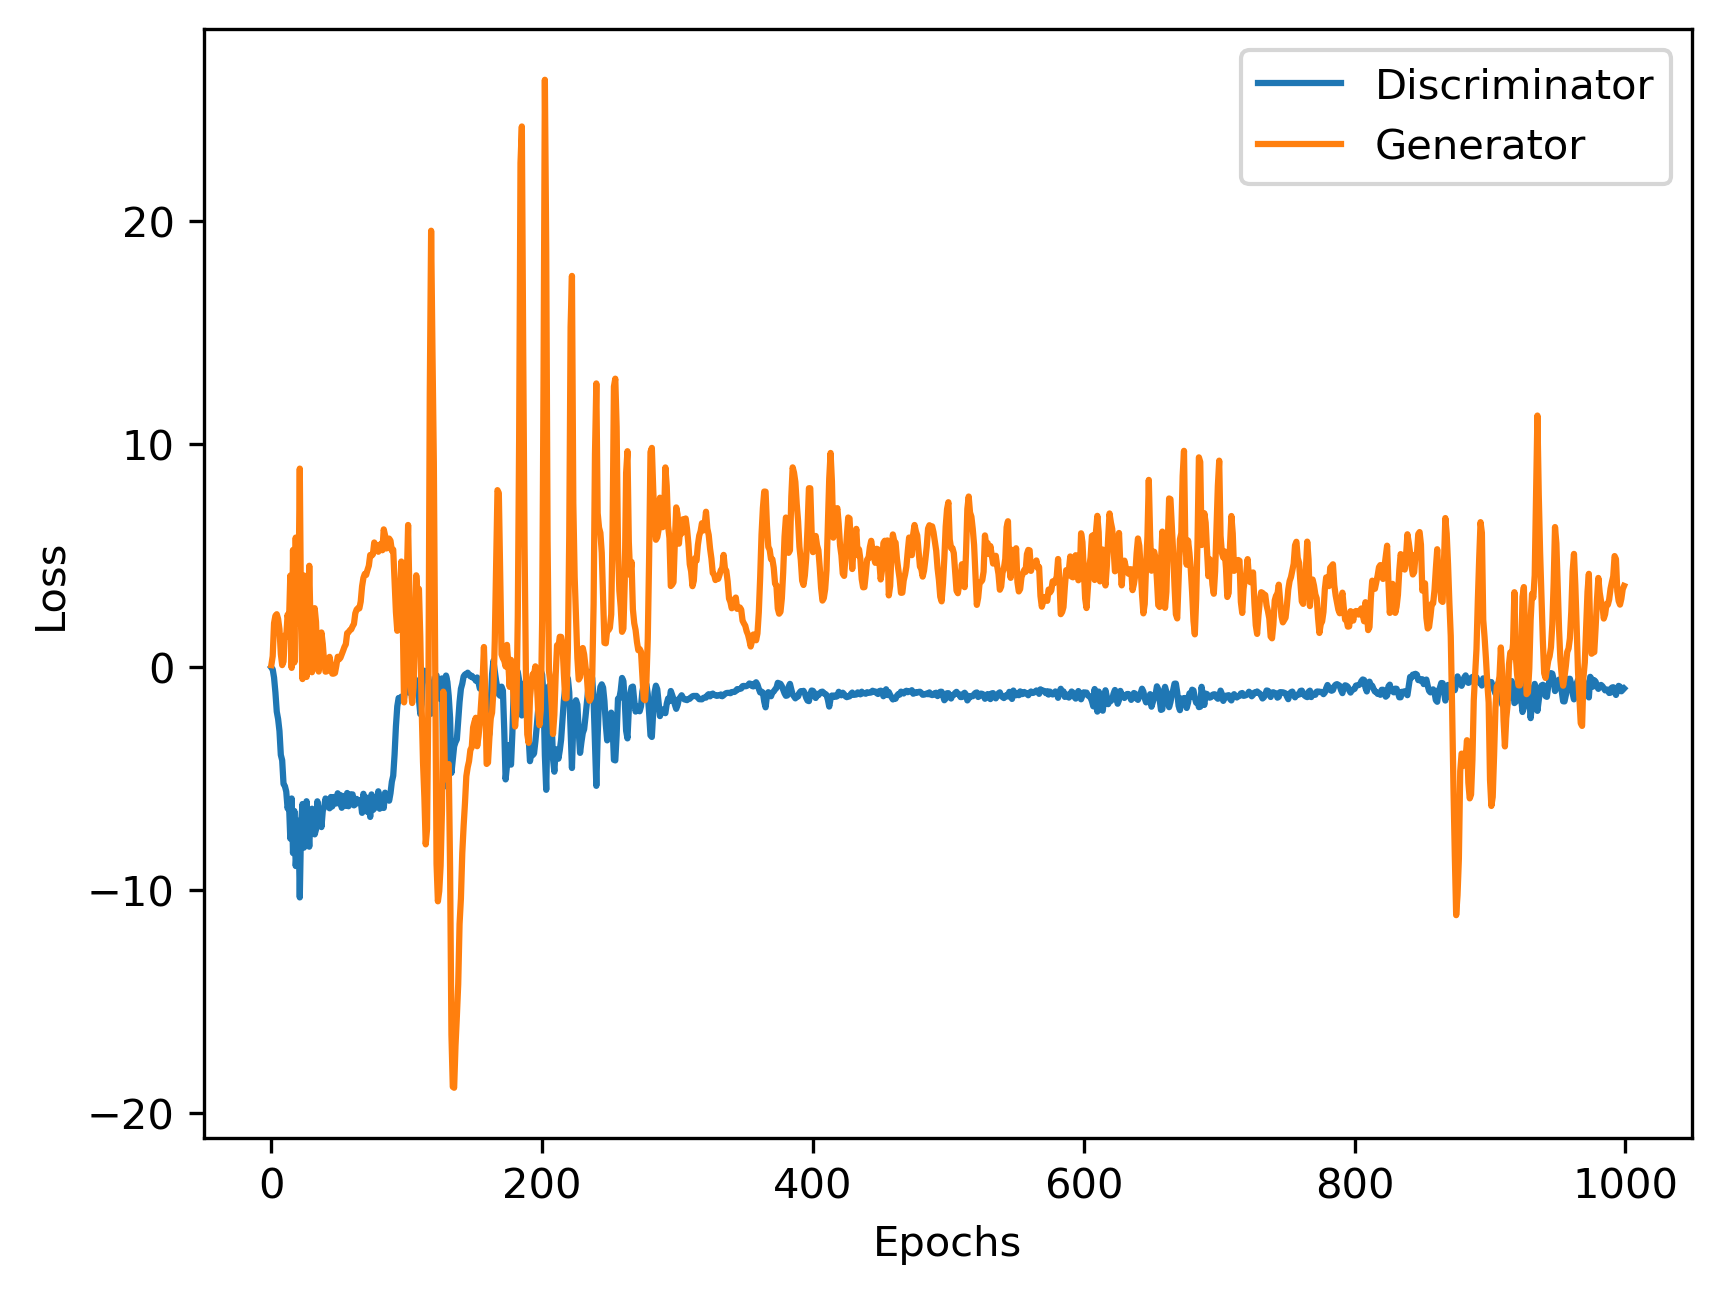
\includegraphics[width=0.45\textwidth]{loss_plots/wpgan_flute_hist_nearest_pitch_0729.png}
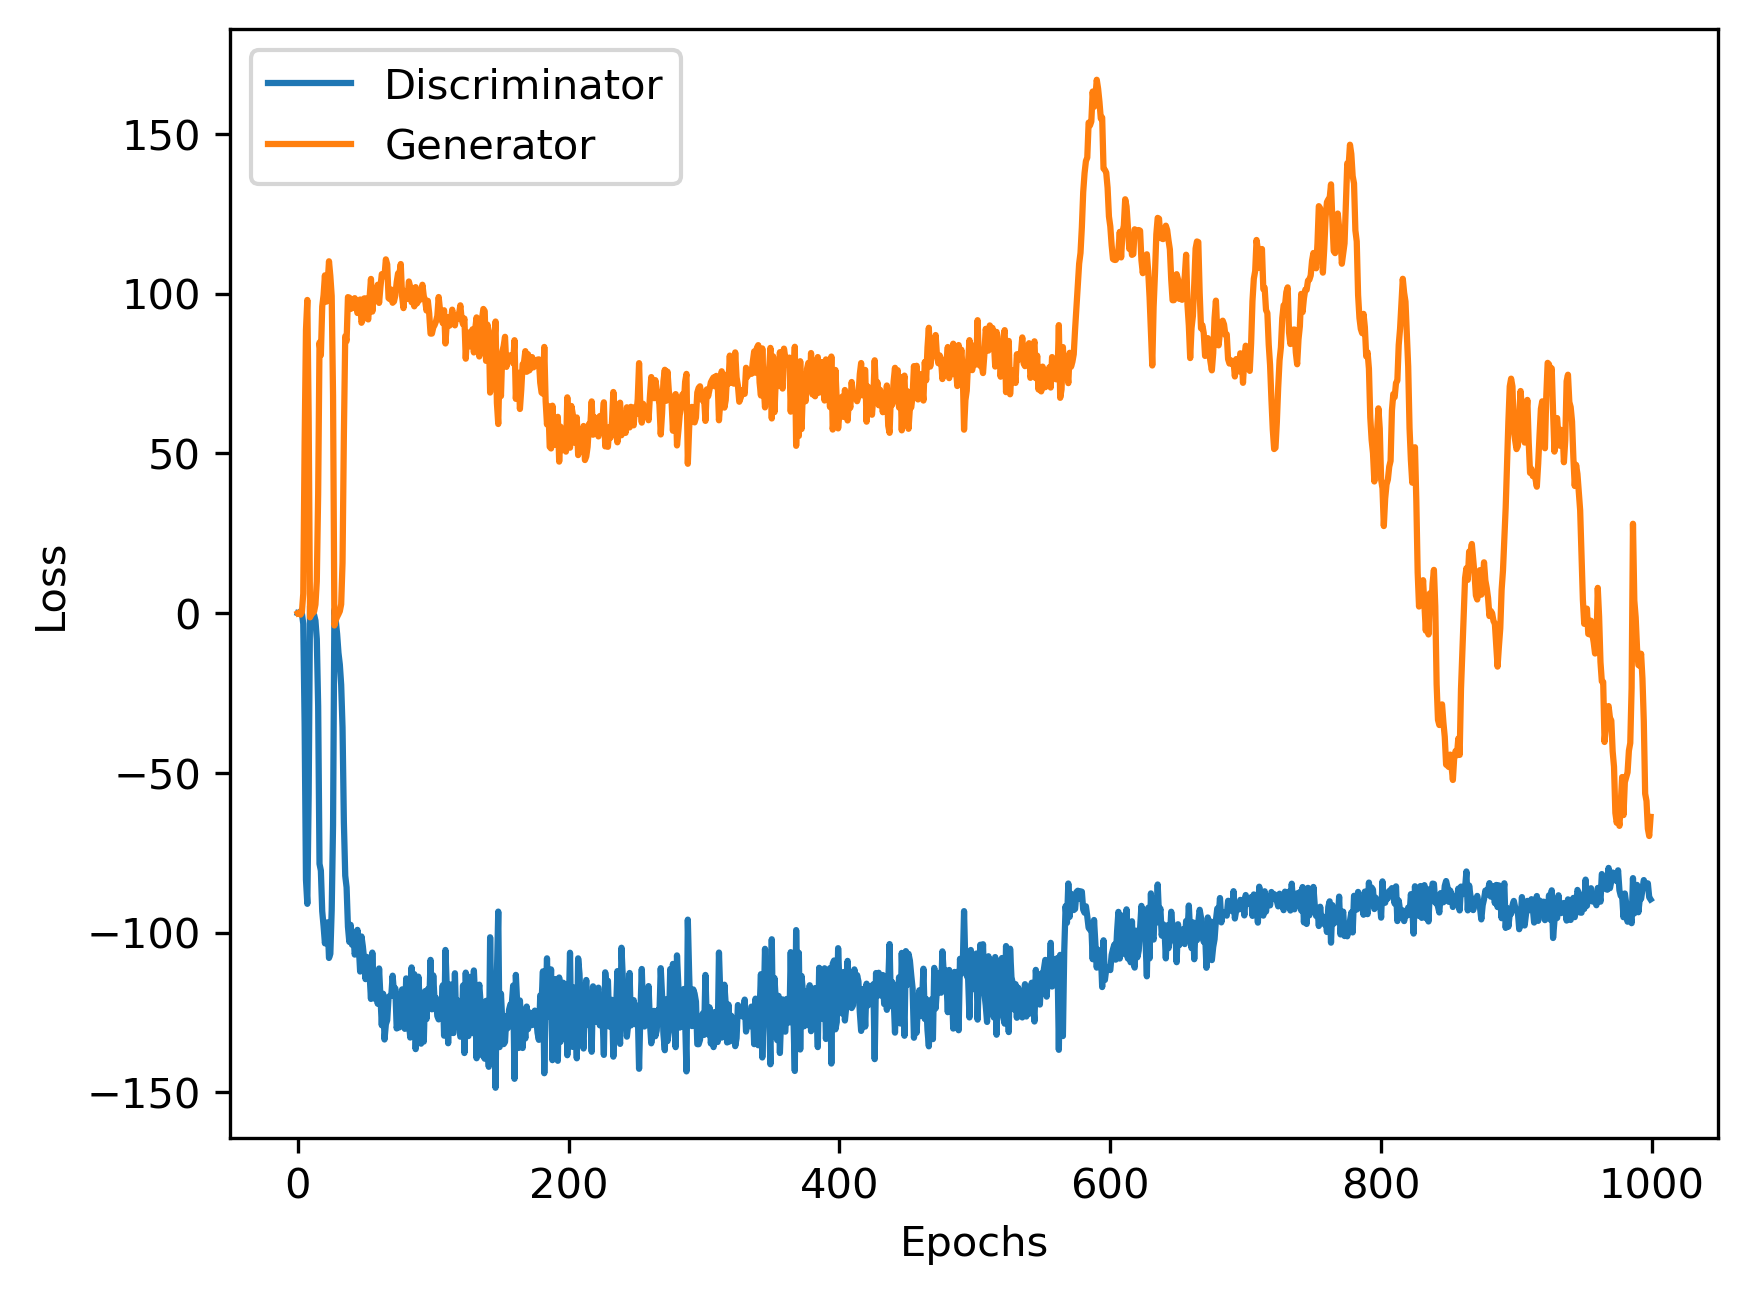
\includegraphics[width=0.45\textwidth]{loss_plots/wpgan_flute_hist_nearest_nonorm_pitch_0729.png}
\caption{Left: Nearest neighbour interpolation, Right: Nearest neighbour interpolation with no batch normalization}
\end{figure*}

\begin{figure*}[t]
\centering
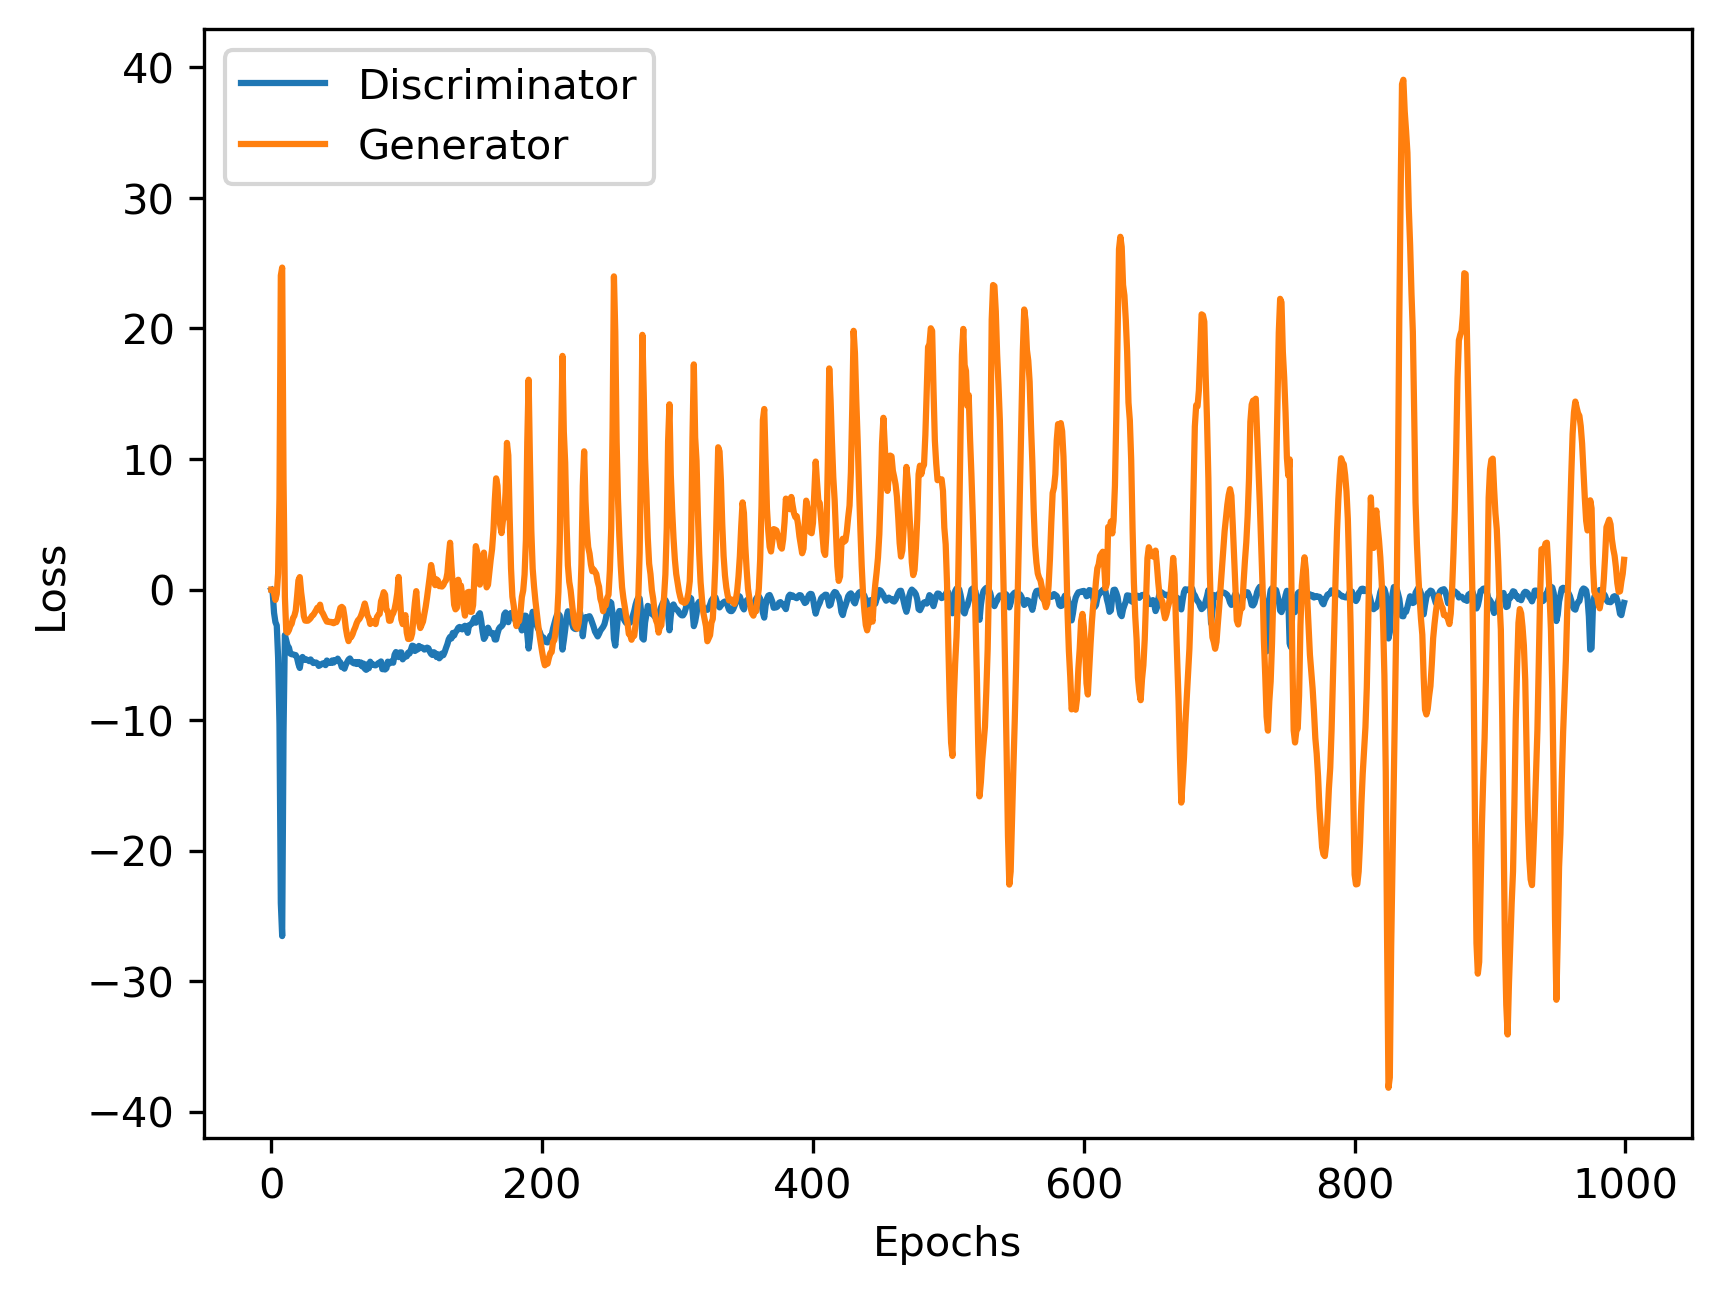
\includegraphics[width=0.45\textwidth]{loss_plots/wpgan_flute_hist_nonorm_pitch_0729.png}
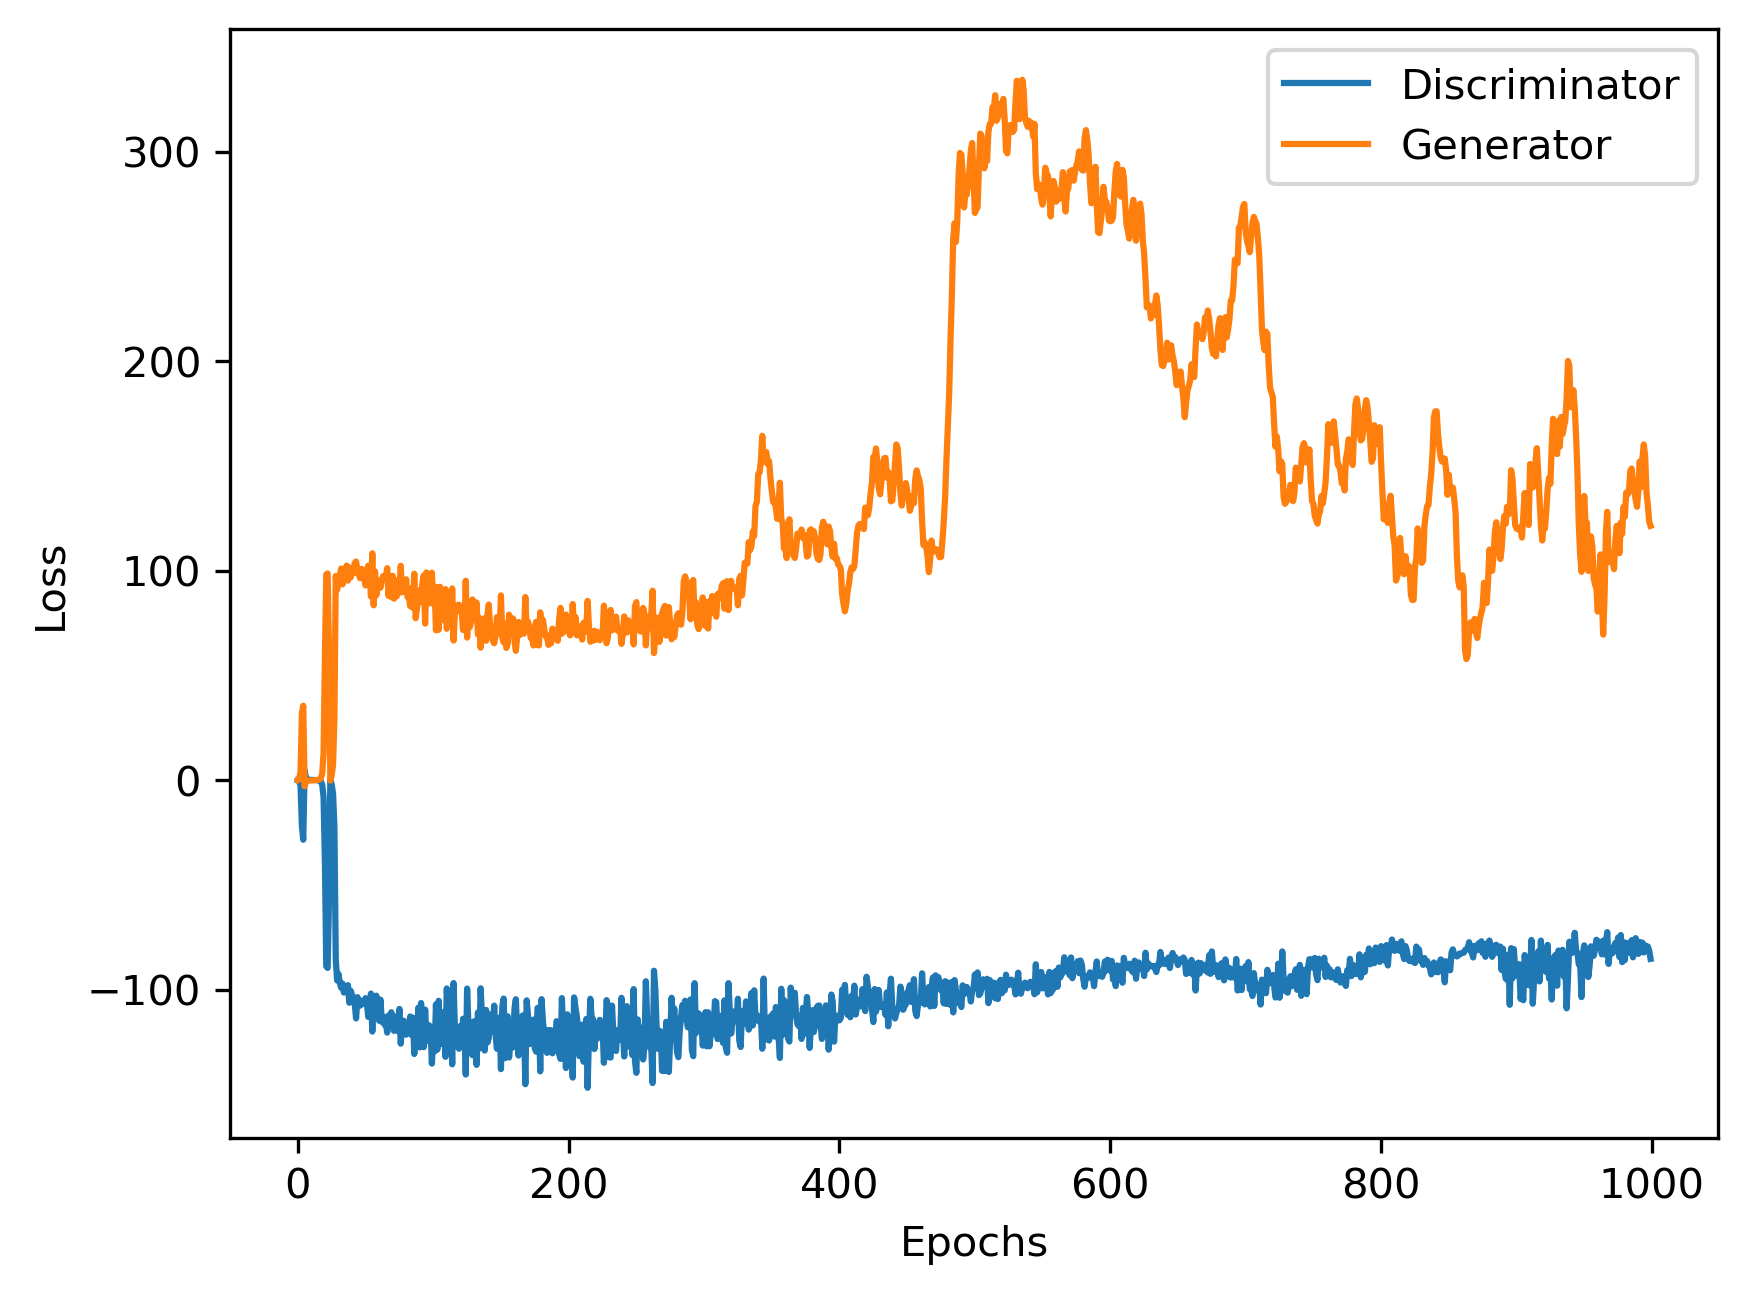
\includegraphics[width=0.45\textwidth]{loss_plots/wpgan_flute_hist_upsample_nonorm_pitch_0729.png}
\caption{Left: Transpose convolution with no batch normalization, Right: Upsample layer with no batch normalization}
\end{figure*}

\begin{figure*}[t]
\centering
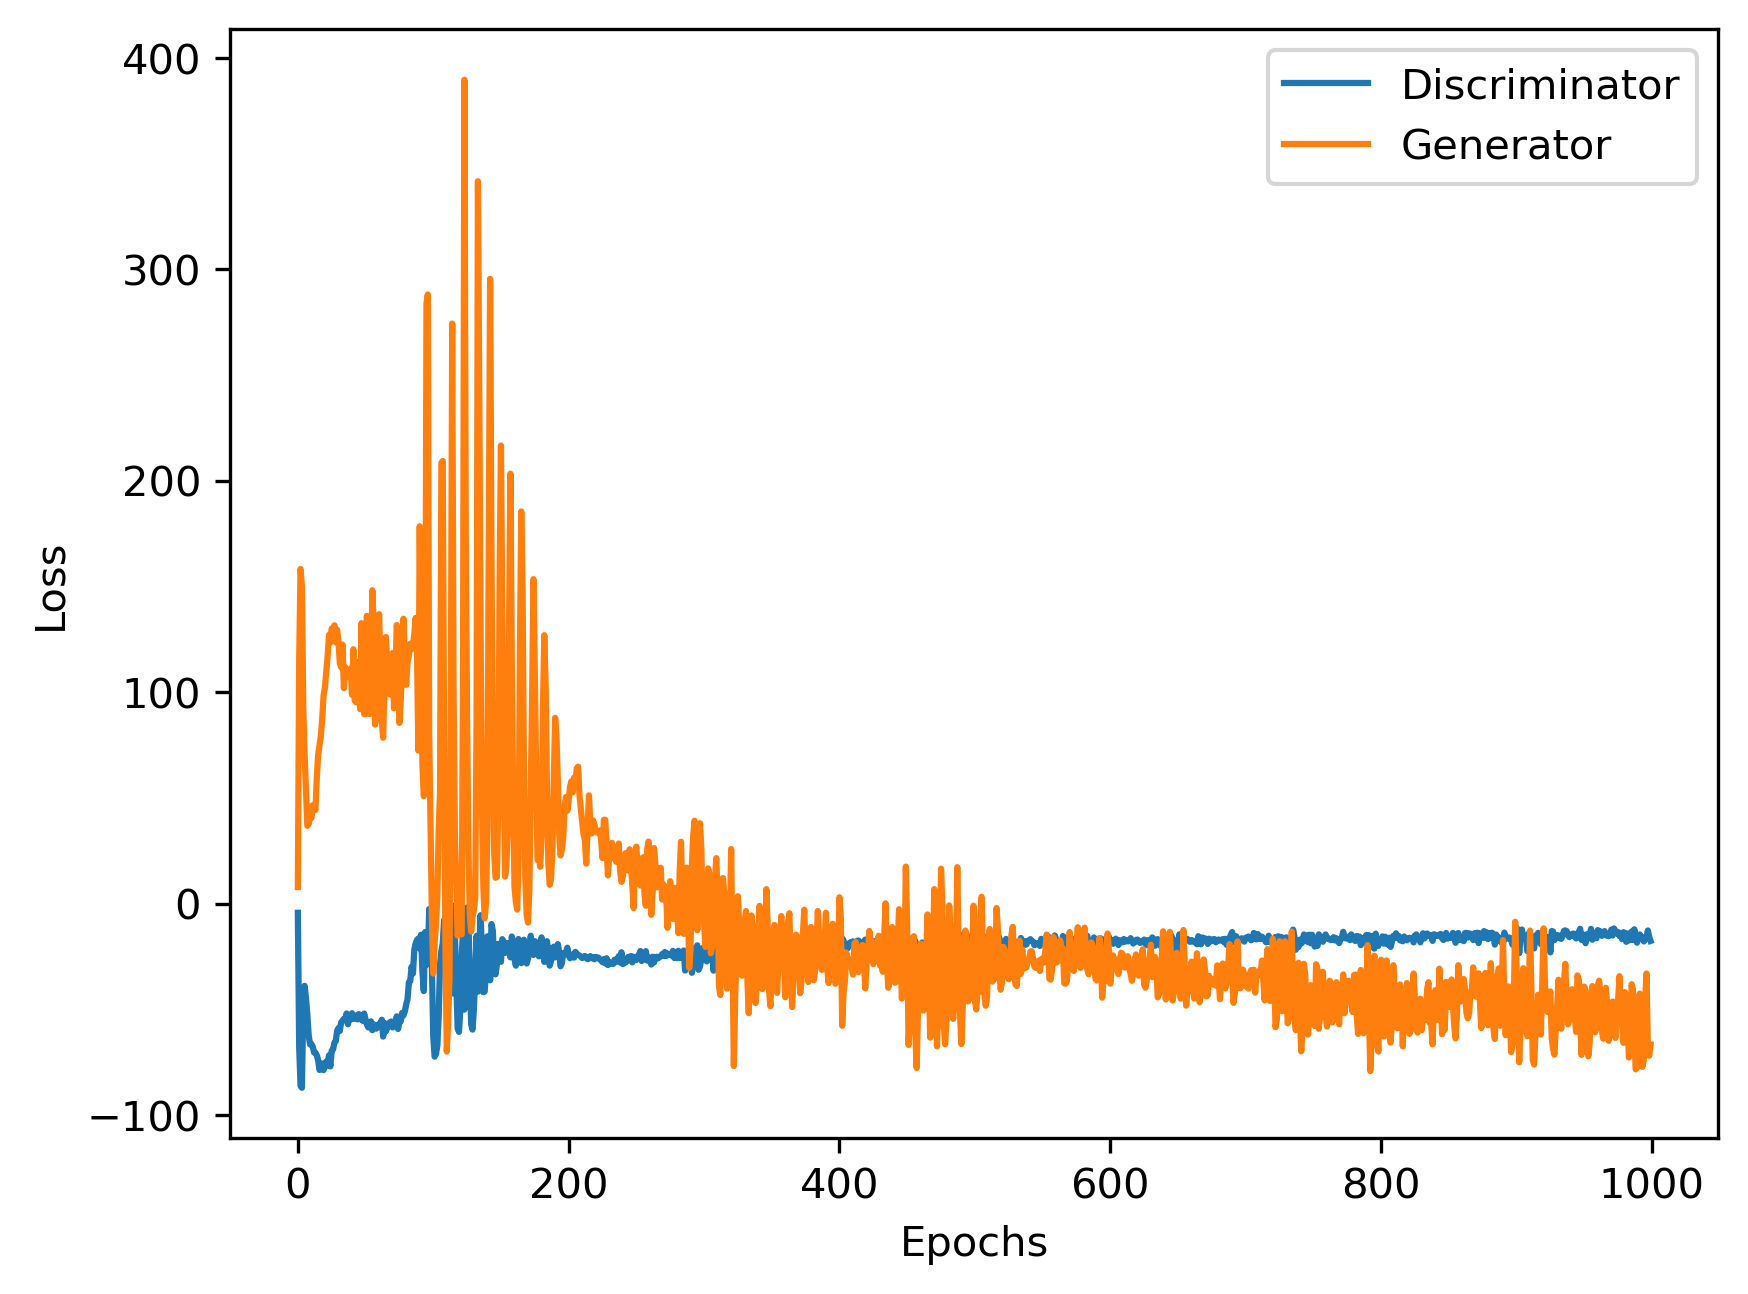
\includegraphics[width=0.45\textwidth]{loss_plots/wpgan_flute_hist_nearest_k5_d50_0803.png}
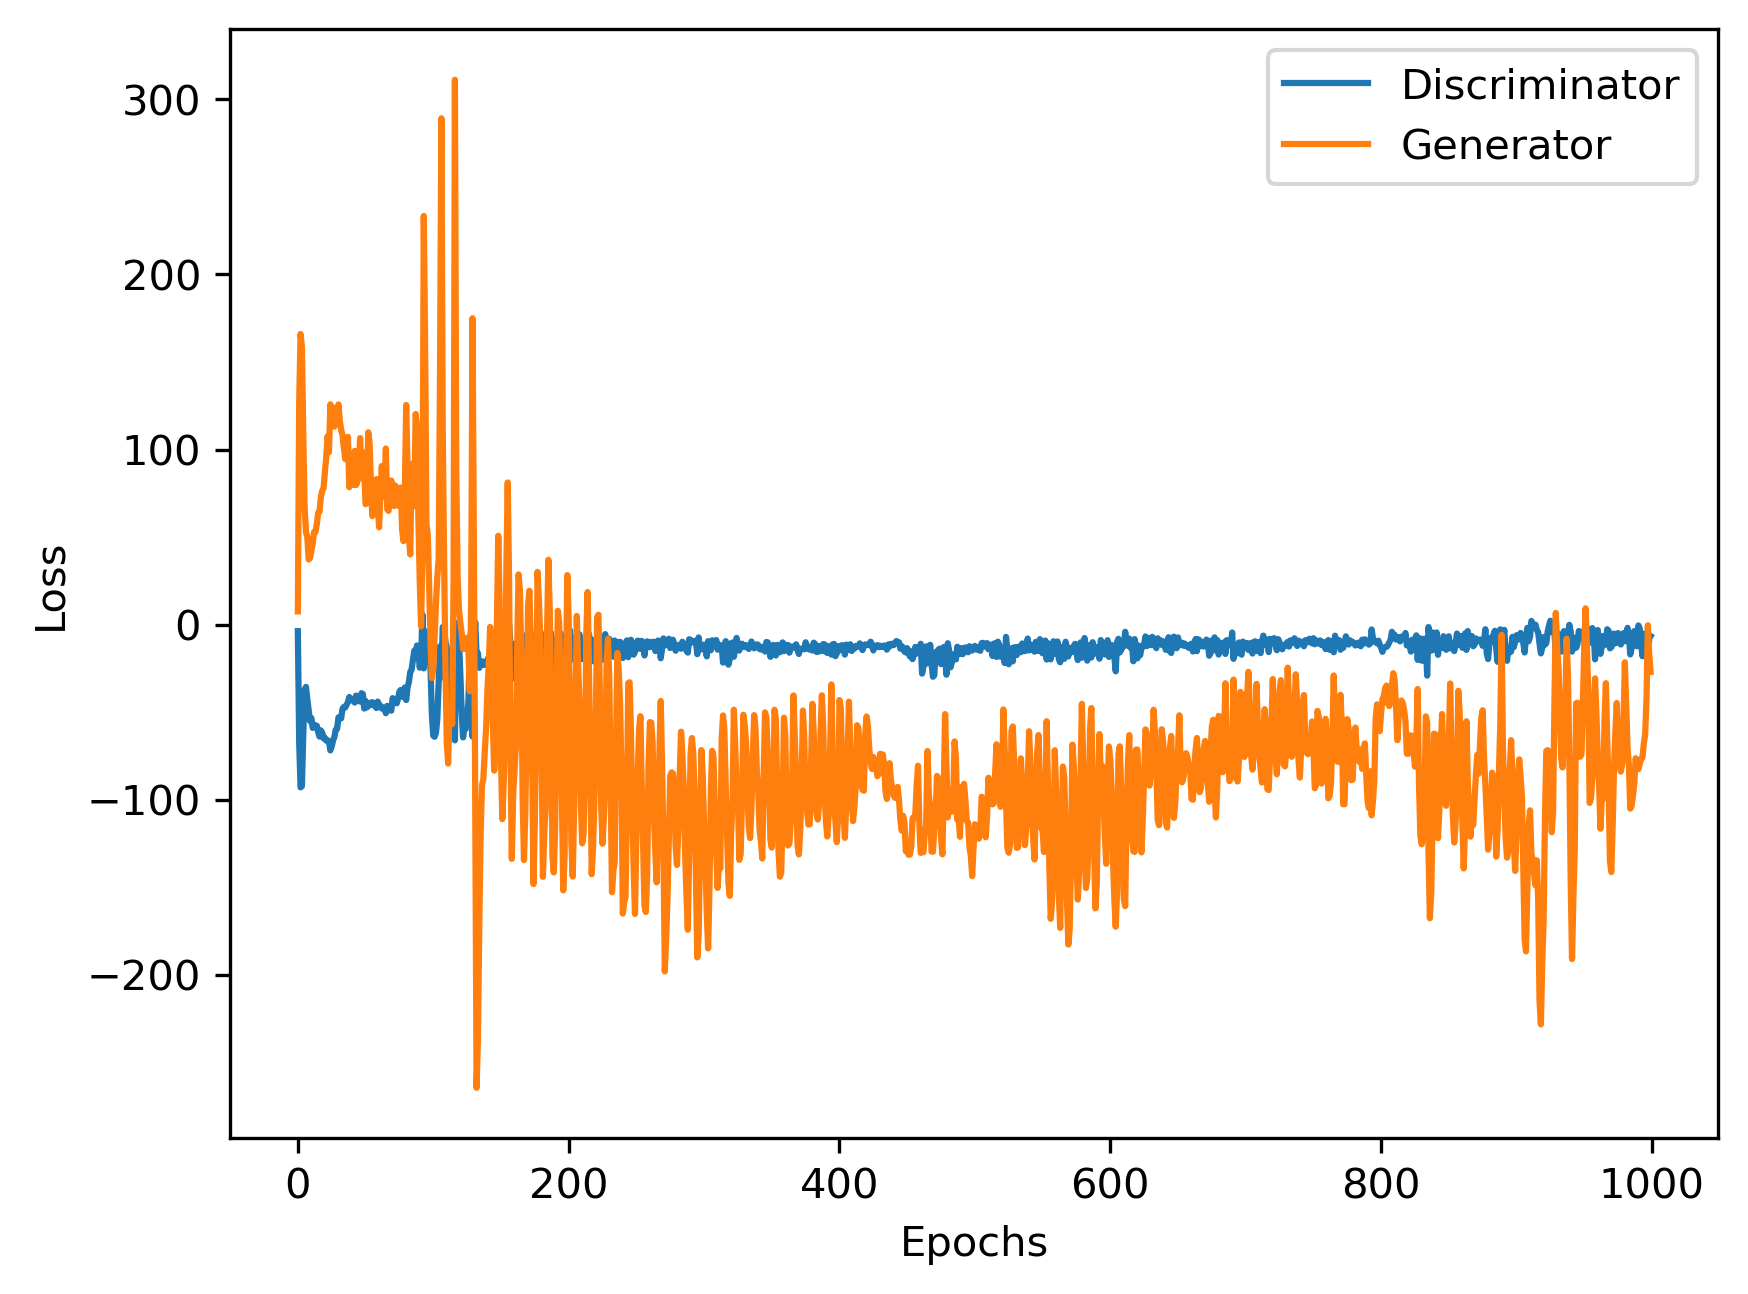
\includegraphics[width=0.45\textwidth]{loss_plots/wpgan_flute_hist_nearest_ps_k5_d50_0803.png}
\caption{Left: Nearest neighbour interpolation and a dropout of 50\% in the generator. Right: Nearest neighbour interpolation, dropout of 50\% in the generator, and phase shuffling.}
\end{figure*}

\begin{figure*}[t]
\centering
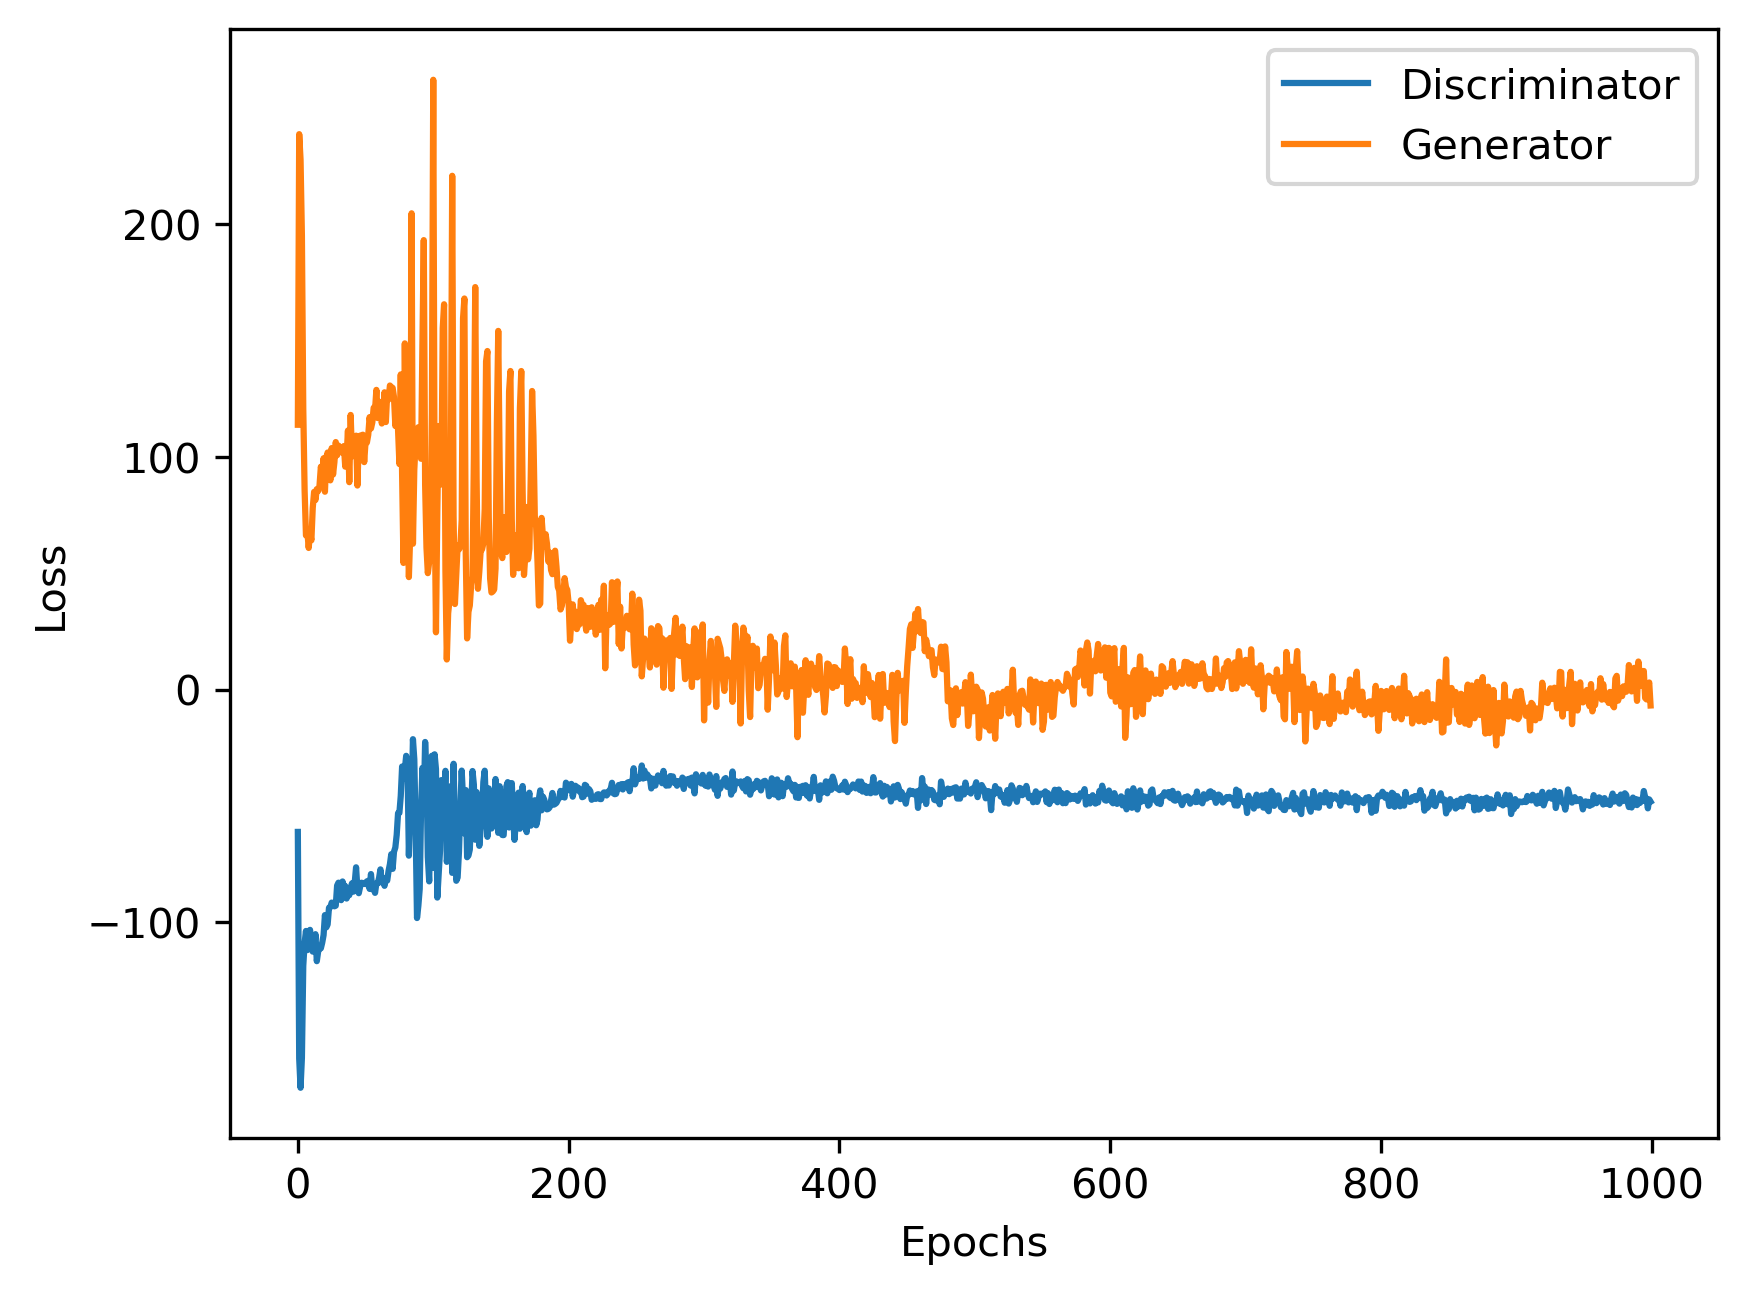
\includegraphics[width=0.45\textwidth]{loss_plots/wpgan_flute_hist_nearest_k15_d50_0803.png}
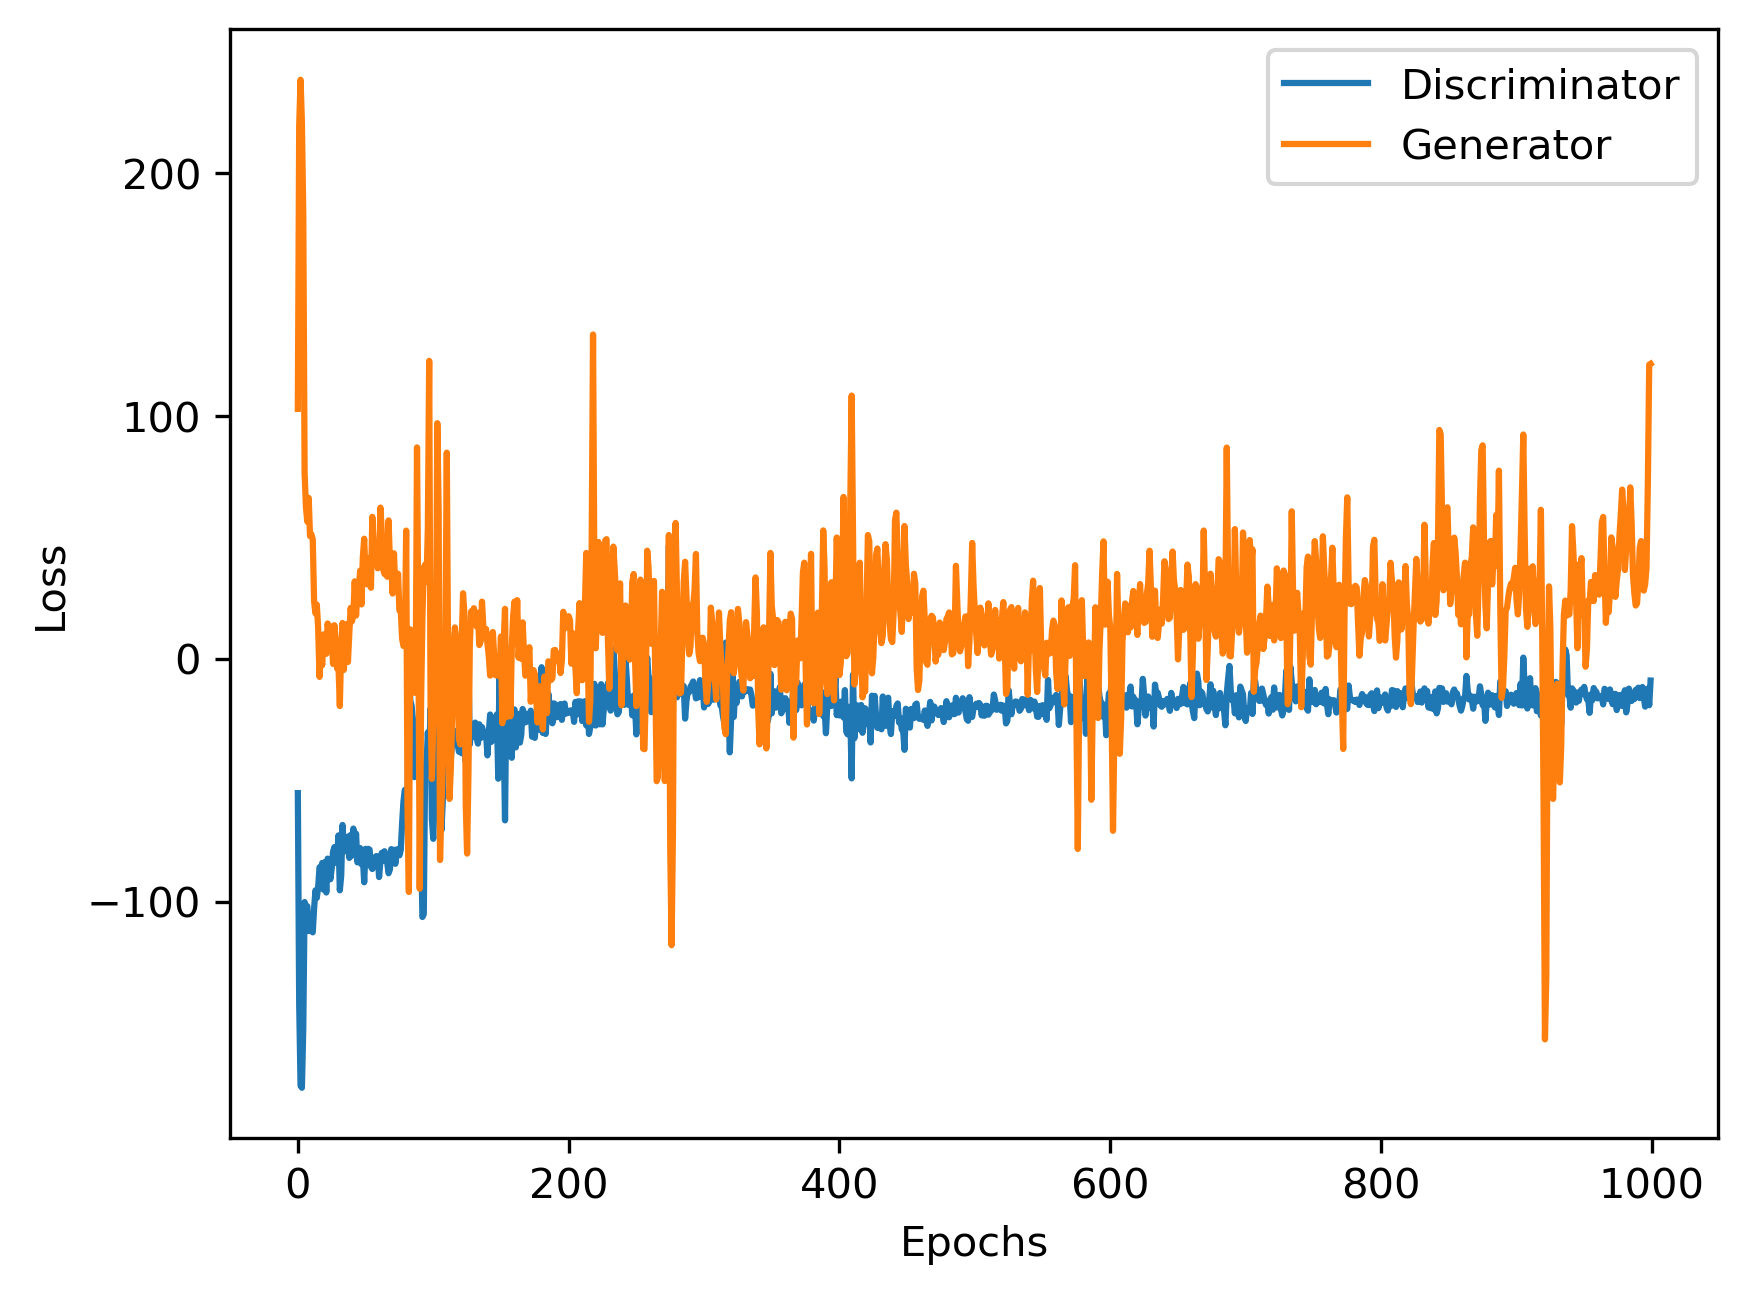
\includegraphics[width=0.45\textwidth]{loss_plots/wpgan_flute_hist_nearest_ps_k15_d50_0803.png}
\caption{Left: Nearest neighbour interpolation and a dropout of 50\% in the generator, discriminator kernel size of 15. Right: Nearest neighbour interpolation, dropout of 50\% in the generator, phase shuffling, and discriminator kernel size of 15}
\end{figure*}

\begin{figure*}[t]
\centering
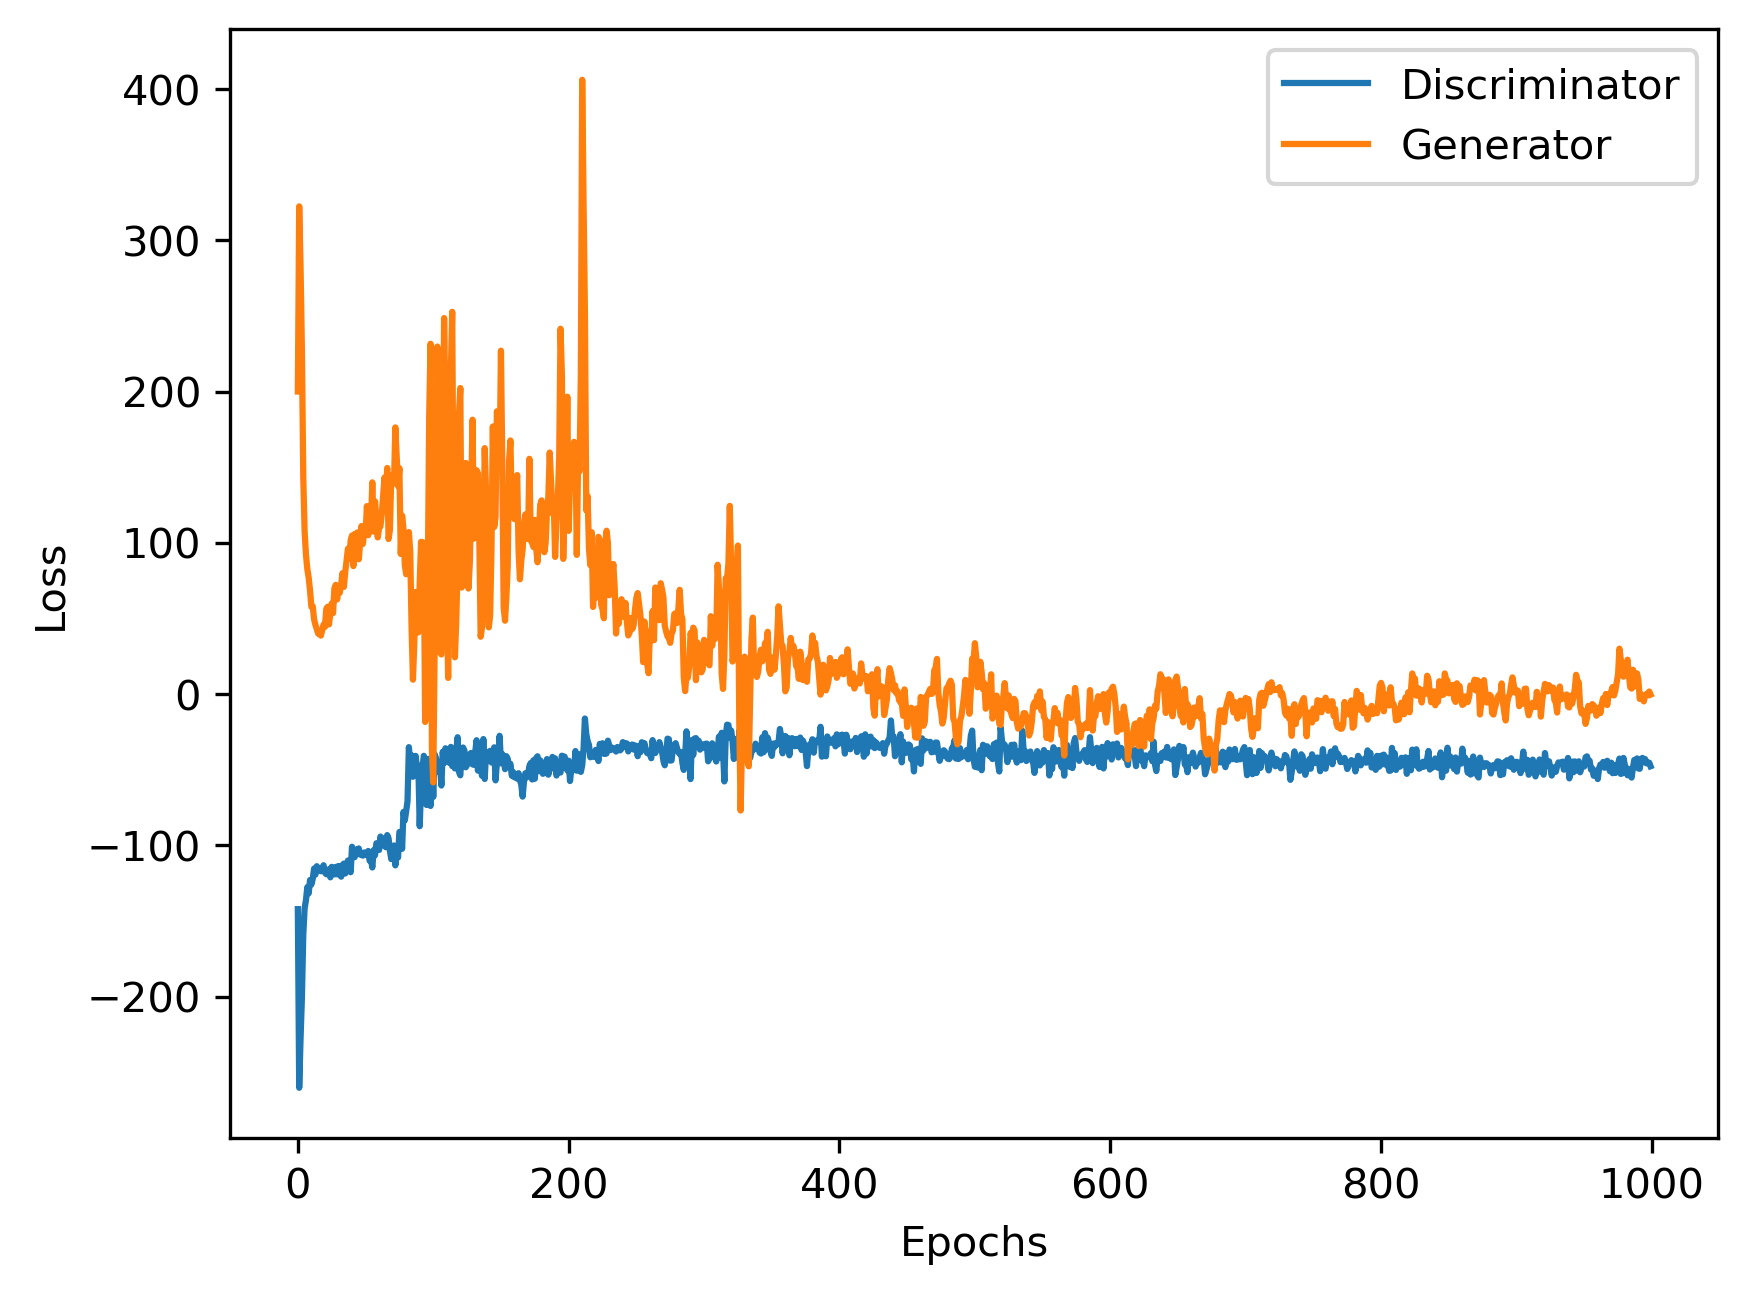
\includegraphics[width=0.45\textwidth]{loss_plots/wpgan_flute_hist_nearest_d50_0803.png}
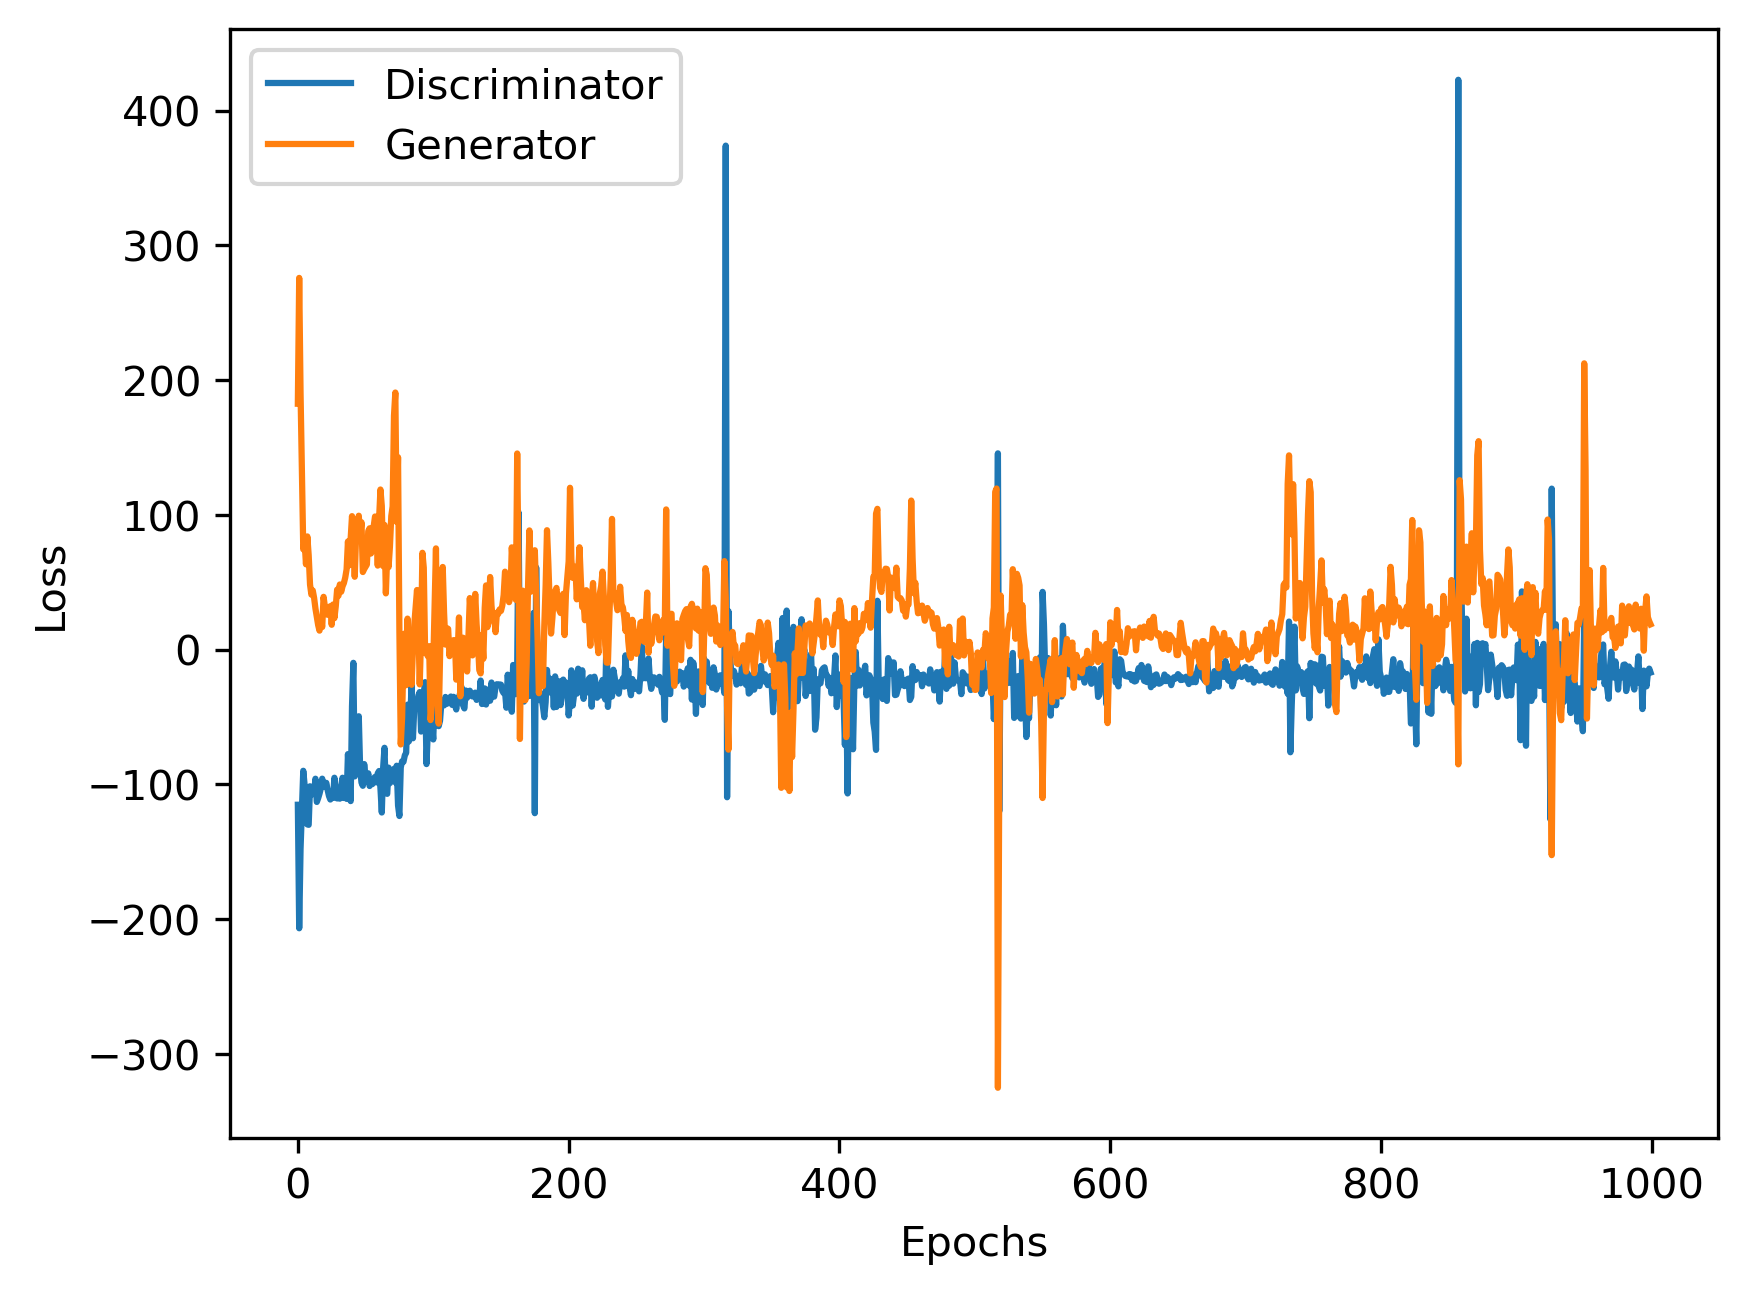
\includegraphics[width=0.45\textwidth]{loss_plots/wpgan_flute_hist_nearest_ps_d50_0803.png}
\caption{Left: Nearest neighbour interpolation and a dropout of 50\% in the generator, discriminator kernel size of 25. Right: Nearest neighbour interpolation, dropout of 50\% in the generator, phase shuffling, and discriminator kernel size of 25}
\end{figure*}

	
%   From the starter document
% 	\startchapter{The Problem to be Solved}
\label{chapter:problem}

\newlength{\savedunitlength}
\setlength{\unitlength}{2em}

Here is where you tell me what is the problem you have been working on for the past few months (or years). I want all the details and you should not be timid about being too tutorial, except that you do not want to cross the line towards writing a textbook. However consider carefully that \textit{communication} implies conveying ideas to other people, while \textit{effective communication} occurs when your message is clearly understood. Remember that your audience must understand your message before they can agree with you.

Ask yourself:
\textit{who is your audience?} You might think of your supervisor who knows everything and you want to impress with your knowledge. I think instead of the graduate students who will be reading this thesis which is, after all, a property of the university. It is published as a university technical report so that others may learn by reading it. Then teach them! Be a bit tutorial. Even the expert external examiner will be impressed by your clarity of exposition if he or she does not need to read paragraphs twice in order to understand - something which people with PhDs and big egos find particularly irritating.

On the other hand, do not go too far and give trivial definitions from concepts learned in a 3rd year undergraduate courses, else you might find yourself in trouble when having to remember the details during an oral examination.

My approach is to put everything necessary to make clarity for
the problem the main goal of this chapter, assuming an intelligent and well prepared reader who already has a Bachelor degree in an appropriate subject.

Once I understand the problem clearly and its nuances (it may not be what I expected after all), I also need to know why the problem is important, what its impact is and what its application, if any. Here you are free to elaborate and write as much as you think is necessary to avoid the examination doubt that you have a brilliant new solution to a trivial and unimportant issue.

I suggest reading various books on how to do research and set up problems. The best for me was "The Craft of Research" by Wayne Booth \cite{booth1}, which can be found in the main library at Q180.55 M4B66. From there I have transferred to my writing a fairly simple structure for talking about the topic of the research, with the question to be asked and its motivation and significance. It goes as follows:
\begin{enumerate}
\item {\textit{I am trying to learn about (working on, studying...)}}
\item {\textit{because I want to find out....}}
\item {\textit{in order to understand...}}
\end{enumerate}

Another way of looking at this is to ask the
\textit{what}, \textit{why} and \textit{where}, starting from a \textit{setting} of the problem with a first point A, stating what the \textit{goal} is at point B and having an \textit{action link} between the two which will encompass your new solution. As surprising as this may be to some of you, I found reading a book from Microsoft very useful: "Beyond Bullet Points: Using Microsoft Office PowerPoint 2007 to Create Presentations That Inform" \cite {atkin}. The goal of the book is to improve presentations with Power Point, but there is a lot that can be transferred towards \textit{effective communication} for a thesis.

In summary, my view of the second chapter on
\textit{"The Problem to be solved"} is as follows:
\begin{enumerate}
\item {\textit{Not} all the background and definitions (boring!) - use instead just-in-time explanations as needed in every context as it comes up;}
\item {Motivation in depth;}
\item {Tutorial high level explanation, where it is important to choose the right pitch: who is the audience? who are you teaching here?}
\item {Make it exciting, make it current, make it important - why do I want to keep reading?}
\item {Should you list here the solutions from other researchers? I think not, list instead the different facets of the problems that other researchers have attacked.}
\item {A taxonomy can be extremely useful to place your problem and its particular special features within the perfect context of the overall area, as you need to make sure that the reader understands perfectly what you are trying to solve.}
\end{enumerate}


\setlength{\unitlength}{\savedunitlength}

% 	\startchapter{The New Approach and Solution}
\label{chapter:newsol}

This is where you go all out and tell us all about your new discovery and research related to the problem in the previous chapter. No arrogant sweeping statements which cannot be fully justified, but no false modesty either. You must impress your reader that you have accomplished something.

Simply summarized, this chapter should be comprised of at least two main sections, each with appropriate subsections. The first section should describe:
\begin{itemize}
\item {what the new approach is;}
\item {what is really totally new;}
\item {what is incrementally new;}
\item {what you built upon.}
\end{itemize}

The second part should describe fully how the new approach works, both with the overall theoretical exposition (e.g. an algorithm) and with as many examples as necessary for clarity. Remember that if the reader does not understand fully, you will get a lot of questions and doubts. Good examples, good figures, good diagrams with super clear tutorial explanations can be a joy to read and make even a small contribution appear to be more impressive. Are you afraid that if you are too tutorial your work will not seem as deep and difficult? Only shallow people will make such a superficial evaluation, have trust instead in the wisdom of your supervisory committee.

Use at least one good example throughout, and even better if this is one of the examples you used in Chapter 2 to describe the original problem.

By the way, this would be the first chapter I would write. This is what I know best right now, as I just finished working on it. It is clear to me and on the tip of my fingers. Start with your strengths! The second chapter I would write is the next one about the experiments, followed closely by chapter 2 describing the problem. It may not seem intuitive to you, but it works and it is the most productive way I ever found to finish a document.


\input chapters/3/sec_latexhelp

% 	\startchapter{Experiments}
\label{chapter:Exp}

Assuming you have some experimental results to support your claims this is where all the data is reported. There are a few issues you should consider before dumping a lot of stuff here, or it will lose its effectiveness.

First of all you must describe precisely the experimental setup and the benchmarks you used. In any scientific discipline an experimental result is only good if it is reproducible. To be reproducible then somebody else must have sufficient details of the setup to be able to obtain the same data. Thus the first section in this chapter is a super precise history of the decisions made towards experimentation, including mentions of the paths which became infeasible. The setup must be valid and thus your description of it must prove that it is indeed sound. At times, terrifying times, when writing this section, both supervisor and student realize belatedly that something is missing and more work needs to be done!

The second portion of this chapter is dedicated the the actual results. At least two issues arise here:
\begin{enumerate}
\item {Should all the data be reported here or should some be placed in the Appendix?}
\item {Should this be an exposition of the raw facts and data or should it include its analysis and evaluation?}
\end{enumerate}

There are no definite answers here, but I follow a few rules.

\textit{Should all the data be reported here or should some be placed in the Appendix?}
    \begin{itemize}
    \item{If there is a large number of tables of data, it might be better to present here only a handful of the most significant ("best") results, leaving all the rest of the data in the Appendix with proper linkages, as it would make the chapter so much more easily readable (not to mention limiting the struggle with a word processor for the proper placement of tables and text).}
    \item{Use an example throughout, call it a "case study" to make it sound better, so that all the data and results are somehow linked in their logic, and even better if this is one of the examples you used in Chapter 2 to describe the original problem.}
    \item{Highlight in some manner the important new data, for example the column of your execution speed where all the numbers are much smaller. Make the results highly easy to read!}
    \item{It is normally expected that data should be presented only in one form and not duplicated, that is, you are not supposed to include both a table of raw numbers and also its graphical representation from some wonderful Excel wizard. I tend to disagree. I would not wish to see every results repeated in this manner, but some crucial ones need to be seen in different manners, even with the same information content, in order to show their impact. One good trick is to place the more boring tables in the Appendix and use wonderful graphs in this chapter.}
    \item{This is the one chapter where I would splurge and use colour printing where necessary, as it makes an \textit{enourmous} difference.}
    \end{itemize}

\textit{Should this be an exposition of the raw facts and data or should it include its analysis and evaluation?}
     \begin{itemize}
    \item{Is the evaluation of the data really obvious? For example you have 10 tables to show that your chemical process is faster in development and gives purer material - you may simply need to highlight one column in each table and state the obvious.}
    \item{Most results are not that obvious even if they appear so. Moreover this is where you are comparing your \textit{new} results to data from other people. I usually describe other people's work at this point and make comparisons. That is why I prefer to talk about the analysis and evaluation of the results in a separate chapter.}
    \item{There is absolutely no clear structure here which is best.}
    \end{itemize}

% 	\startchapter{Evaluation, Analysis and Comparisons}
\label{chapter:eval}

For a Master's research this chapter represents the critical part where \textbf{you} are truly evaluated to determine whether you should be given your degree. Even more so for a PhD. Consider carefully what the University calendar states regarding the expectations for a master's thesis, paraphrased here.

\begin{enumerate}
\item {\textit{A Master?s thesis is an original lengthy essay.} The main implication here is that the essay is original, that is, it is completely newly written by you and does not contain any writings from others unless precisely quoted. Any paraphrased items must be cited.}
\item {\textit{It must demonstrate that:}
    \begin{itemize}
    \item {students understand research methods;}
    \item {students are capable to employ research methods;}
    \item {students demonstrate command of the subject.}
    \end{itemize}}
\item {\textit{The work may be based on:}
    \begin{itemize}
    \item {original data;}
    \item {original exercise from scholarly literature;}
    \item {data by others.}
    \end{itemize}}
\item {\textit{The work must show that:}
    \begin{itemize}
    \item {appropriate research methods have been used;}
    \item {appropriate methods of critical analysis supplied.}
    \end{itemize}}
\item {\textit{The work must contain:}
    \begin{itemize}
    \item {evidence of some new contribution;}
    \item {evidence of a new perspective on existing knowledge.}
    \end{itemize}}
\end{enumerate}

Only the last point uses the attribute \textit{new} and it refers almost entirely to giving a new perspective and analysis, even if based on data from others. This truly implies that this current chapter on evaluation and analysis of results is the most important and must be written with care. You are demonstrating here that, even if given data and methods from others, your skills of critical judgment and analysis are now at the level that you can give professional evaluations.

Things are slightly different for a PhD. According to the Graduate Calendar: \\ 
\textit{a doctoral dissertation must embody original work and constitute a significant contribution to knowledge in the candidate's field of study. It should contain evidence of broad knowledge of the relevant literature, and should demonstrate a critical understanding of the works of scholars closely related to the subject of the dissertation. Material embodied in the dissertation should, in the opinion of scholars in the field, merit publication.}

\textit{The general form and style of dissertations may differ from department to department, but all dissertations shall be presented in a form which constitutes an integrated submission. The dissertation may include materials already published by the candidate, whether alone or in conjunction with others. Previously published materials must be integrated into the dissertation while at the same time distinguishing the student's own work from the work of other researchers. At the final oral examination, the doctoral candidate is responsible for the entire content of the dissertation. This includes those portions of co-authored papers which comprise part of the dissertation.}

The second paragraph makes it clear that one must emphasize what is new and different from others, without arrogance, yet without being too subtle either. The first paragraph implies that for a PhD it is required that one approached an important open problem and gave a new solution altogether, making chapters 3, 4, 5 all part of the body of research being evaluated. In fact at times even the problem may be entirely new, thus including chapter 2 in the examination. This is in contrast to a Master's degree where the minimum requirement is for chapter 5 to be original.




% 	\startchapter{Conclusions}
\label{concl}

My first rule for this chapter is to avoid finishing it with a section talking about future work. It may seem logical, yet it also appears to give a list of all items which remain undone! It is not the best way psychologically.

This chapter should contain a mirror of the introduction, where a summary of the \textit{extraordinary} new results and their wonderful attributes should be stated first, followed by an executive summary of how this new solution was arrived at. Consider the practical fact that this chapter will be read quickly at the beginning of a review (thus it needs to provide a strong impact) and then again in depth at the very end, perhaps a few days after the details of the previous 3 chapters have been somehow forgotten. Reinforcement of the positive is the key strategy here, without of course blowing hot air.

One other consideration is that some people like to join the chapter containing the analysis with the only with conclusions. This can indeed work very well in certain topics.

Finally, the conclusions do not appear only in this chapter. This sample mini thesis lacks a feature which I regard as absolutely necessary, namely a short paragraph at the end of each chapter giving a brief summary of what was presented together with a one sentence preview as to what might expect the connection to be with the next chapter(s). You are writing a story, the \textit{story of your wonderful research work}. A story needs a line connecting all its parts and you are responsible for these linkages.

% 	\appendix
% 	\startappendix{Additional Information}
\label{chapter:appendix}

This is a good place to put tables, lots of results, perhaps all the data compiled in the experiments. By avoiding putting all the results inside the chapters themselves, the whole thing may become much more readable and the various tables can be linked to appropriately.

The main purpose of an Appendix however should be to take care of the future readers and researchers. This implies listing all the housekeeping facts needed to continue the research. For example: where is the raw data stored? where is the software used? which version of which operating system or library or experimental equipment was used and where can it be accessed again?

Ask yourself: if you were given this thesis to read with the goal that you will be expanding the research presented here, what would you like to have as housekeeping information and what do you need? Be kind to the future graduate students and to your supervisor who will be the one stuck in the middle trying to find where all the stuff was left!



% The style of bibliography exemplified here is the "plain",
% normally used in science theses. This is shown
% by the entry {plain} below. Substitute the
% appropriate bibliography style. See also the
% PDF file "InformationOnBibliographyStyles" in this
% directory for more choices.

% The Bibliography file is a BibTex file named
% UVicThesis.bib and called below

	\TOCadd{Bibliography}
	\bibliographystyle{plain}
	\bibliography{refs}

\end{document}
